
%--------------------------------------------------------------------------------------
% Alapbeállítások
%--------------------------------------------------------------------------------------
\documentclass[12pt,a4paper,oneside]{report}
\usepackage[magyar]{babel} % Language support
\usepackage{geometry}
\usepackage{amsfonts,amsmath,amssymb} % Mathematical symbols
\usepackage{microtype} % Imrovements to typesetting
\usepackage{setspace} % For setting line spacing
\usepackage{cmap} % Enables more advenced text copying from the PDF document 
\usepackage{sectsty} % Section heading styling

\usepackage{todonotes}

%\usepackage[backend=biber, sorting=none]{biblatex} % sorting=none a hivatkozások sorrendjéhez
%\addbibresource{mybib.bib} % A BibTeX adatbázisfájlod

\usepackage[unicode]{hyperref} % For hyperlinks in the generated document
\usepackage{booktabs} % For publication quality tables for LaTeX
\usepackage{graphicx} % For figure sizing
\usepackage{wrapfig}
\usepackage{float}
\usepackage[hang]{caption}
\usepackage{xcolor} % For code coloring in listings
\usepackage{listings} % For source code snippets
\usepackage[amsmath,thmmarks]{ntheorem} % Theorem-like environments

\usepackage[numbers]{natbib} % Bibliography

%\usepackage[T1]{fontenc} %Betűtípus beállításhoz

\usepackage{fontspec}
\setmainfont{Times New Roman}
\usepackage{lipsum}
\usepackage{tikz}
\usepackage{pdfpages}
%\usepackage{floatrow}

\newcommand{\tss}{\textsuperscript}     % tss = felső index


%--------------------------------------------------------------------------------------
% Elnevezések
%--------------------------------------------------------------------------------------
\newcommand{\elte}{Eötvös Loránd Tudományegyetem}
\newcommand{\ik}{Informatikai Kar}
\newcommand{\smi}{Savaria Műszaki Intézet}

\newcommand{\keszitette}{Horváth Milán}\newcommand{\konzulens}{Konzulens}
\newcommand{\temavezeto}{Témavezető}
\newcommand{\selectbsc}{
  \newcommand{\munkatipus}{Szakdolgozat}       % Dokumentum típusa
  \newcommand{\munkatipusHU}{Szakdolgozat}     % Dokumentum típusa
  \newcommand{\munkatipusok}{Szakdolgozatok}   % többesszámban
  \newcommand{\munkatipustHU}{Szakdolgozatot}  % tárgyraggal
}
\newcommand{\pelda}{Példa}
\newcommand{\definicio}{Definíció}
\newcommand{\tetel}{Tétel}
\newcommand{\jelolesek}{Jelölések jegyzéke}
\newcommand{\eloszo}{Előszó}
\newcommand{\bevezetes}{Bevezetés}
\newcommand{\koszonetnyilvanitas}{Köszönetnyilvánítás}
\newcommand{\osszefoglalas}{Összefoglalás}
\newcommand{\summary}{Summary}
\newcommand{\fuggelek}{Függelék}
\newcommand{\melleklet}{Mellékletek}
\newcommand{\authorName}{\authorFamilyName{} \authorGivenName}
\newcommand{\consulentA}{\consulentATitle\consulentAFamilyName{} \consulentAGivenName}
\newcommand{\consulentB}{\consulentBTitle\consulentBFamilyName{} \consulentBGivenName}
\newcommand{\consulentC}{\consulentCTitle\consulentCFamilyName{} \consulentCGivenName}
\newcommand{\supervisor}{\supervisorTitle\supervisorFamilyName{}
\supervisorGivenName}

\newcommand{\selectthesislanguage}{\selecthungarian}
\newcommand{\selectforeignlanguage}{\selectenglish}


\def\lstlistingname{lista}

\newcommand{\appendixletter}{6} % a fofejezet-szamlalo az angol ABC 6. betuje (F) lesz
\newcommand{\annexletter}{13} % M betű

%--------------------------------------------------------------------------------------
% Oldal elrendezés
%--------------------------------------------------------------------------------------
\pagestyle{plain}
\geometry{inner=35mm, outer=25mm, top=25mm, bottom=25mm}

%--------------------------------------------------------------------------------------
% Szöveg és bekezdés stílus
%--------------------------------------------------------------------------------------
\sectionfont{\Large\upshape\bfseries}  % Section title font
\subsectionfont{\Large\itshape\mdseries}
\subsubsectionfont{\large\itshape\mdseries}
\setcounter{secnumdepth}{3}             % Section numbering depth

\sloppy                                 % Prevent text from spilling over the margin
\widowpenalty=10000 \clubpenalty=10000  % Prevent widow and oprhan rows
\def\hyph{-\penalty0\hskip0pt\relax}    % Enable hyphenation

\onehalfspacing                         % 1.5x Line spacing

\newcommand{\selecthungarian}{
	\selectlanguage{magyar}
	\setlength{\parindent}{2em}			% Paragraph indentation
	\setlength{\parskip}{5pt}			% Paragraph spacing
	\frenchspacing
}

%--------------------------------------------------------------------------------------
% hyperref package beállítás
%--------------------------------------------------------------------------------------
\hypersetup{
    % bookmarks=true,            % show bookmarks bar?
    unicode=true,                % non-Latin characters in Acrobat's bookmarks
    pdfnewwindow=true,           % links in new window
    colorlinks=true,             % false: boxed links; true: colored links
    linkcolor=black,             % color of internal links
    citecolor=black,             % color of links to bibliography
    filecolor=black,             % color of file links
    urlcolor=black               % color of external links
}

%--------------------------------------------------------------------------------------
% Apply variables
%--------------------------------------------------------------------------------------
% This command is called in the main tex file and uses variables set there.
\newcommand{\applyvariables}{
	\author{\authorName}
	\title{\thesisTitle}

	\hypersetup{
		pdftitle={\thesisTitle},     % title
		pdfauthor={\authorName},     % author
		pdfsubject={\munkatipus}, % subject of the document
		pdfkeywords={\keywords},     % list of keywords (separate then by comma)
		pdfproducer={\authorName},   % producer of the document (organization)
		pdfcreator={LaTeX}           % creator of the document (application)
	}
}

%--------------------------------------------------------------------------------------
% Set up listings
%--------------------------------------------------------------------------------------
\definecolor{lightgray}{rgb}{0.95,0.95,0.95}
\lstset{
	basicstyle=\scriptsize\ttfamily, % print whole listing small
	keywordstyle=\color{black}\bfseries, % bold black keywords
	identifierstyle=, % nothing happens
	% default behavior: comments in italic, to change use
	% commentstyle=\color{green}, % for e.g. green comments
	stringstyle=\scriptsize,
	showstringspaces=false, % no special string spaces
	aboveskip=3pt,
	belowskip=3pt,
	backgroundcolor=\color{lightgray},
	columns=flexible,
	keepspaces=true,
	escapeinside={(*@}{@*)},
	captionpos=b,
	breaklines=true,
	frame=single,
	float=!ht,
	tabsize=2,
	literate=*
		{á}{{\'a}}1	{é}{{\'e}}1	{í}{{\'i}}1	{ó}{{\'o}}1	{ö}{{\"o}}1	{ő}{{\H{o}}}1	{ú}{{\'u}}1	{ü}{{\"u}}1	{ű}{{\H{u}}}1
		{Á}{{\'A}}1	{É}{{\'E}}1	{Í}{{\'I}}1	{Ó}{{\'O}}1	{Ö}{{\"O}}1	{Ő}{{\H{O}}}1	{Ú}{{\'U}}1	{Ü}{{\"U}}1	{Ű}{{\H{U}}}1
}

%--------------------------------------------------------------------------------------
% Setup captions
%--------------------------------------------------------------------------------------
\captionsetup[figure]{
	width=.75\textwidth,
	aboveskip=10pt}

\renewcommand{\captionlabelfont}{\it}
\renewcommand{\captionfont}{\footnotesize\it}



%%%%%%%%%%%%%%%%%%%%%%%%%%%%%%%%%%%%%%%%%%%%%%%%%%%%%%%%%%%%%%%%%%%%%%%%%%%%%%%%%%
%%%%%%%%%%%%%%%%%%%%%%%%%%%%%%%%%%%%%%%%%%%%%%%%%%%%%%%%%%%%%%%%%%%%%%%%%%%%%%%%%%
%%%%%%%%%%%%%%%%%%%%%%%%%%%%%%%%%%%%%%%%%%%%%%%%%%%%%%%%%%%%%%%%%%%%%%%%%%%%%%%%%%



\selectbsc 
%--------------------------------------------------------------------------------------
% Változók beállítása [Setting variables]
%--------------------------------------------------------------------------------------
%TODO Állítsd be az alábbi változókat [Set these variables]%
% Szerző [Author]
\def\authorFamilyName{Horváth}
\def\authorGivenName{Milán}
\def\neptun{MYQGQ0}

% Konzulens 1 [Consulent 1]
\def\consulentATitle{}
\def\consulentAFamilyName{Őri}
\def\consulentAGivenName{Zsuzsanna}
\def\consulentARank{termékfejlesztő}

% Konzulens 2 [Consulent 2], ha nincs hagyd üresen
\def\consulentBTitle{}
\def\consulentBFamilyName{Kiss}
\def\consulentBGivenName{Henrik}
\def\consulentBRank{műszaki oktató}

% Konzulens 3 [Consulent 3], ha nincs hagyd üresen 
\def\consulentCTitle{}
\def\consulentCFamilyName{}
\def\consulentCGivenName{}
\def\consulentCRank{}

% Témavezető
\def\supervisorTitle{}
\def\supervisorFamilyName{Bátorfi}
\def\supervisorGivenName{János György}
\def\supervisorRank{egyetemi tanársegéd}

% Dolgozat címe [Thesis title]
\def\thesisTitle{Szakítópofák tervezése lapos próbatesthez}

% Kulcsszavak (a PDF-be) [Keywords (to PDF)]
\def\keywords{mechatronika, szabályozástechnika, etorobotika, ipar 4.0}

% Tanszék [Department]
\def\department{\smi}

% Elzártan kezelendő dolgozat [Restricted access]
%TODO Töltsd ki a korlátozás lejártának dátumát! 
\def\endOfRestrictedAccess{2034 január 31. nap}

% Változók beállítása a PDF fájlhoz [Apply variables for the PDF file]
\applyvariables



%%%%%%%%%%%%%%%%%%%%%%%%%%%%%%%%%%%%%%%%%%%%%%%%%%%%%%%%%%%%%%%%%%%%%%%%%%%%%%%%%%
%%%%%%%%%%%%%%%%%%%%%%%%%%%%%%%%%%%%%%%%%%%%%%%%%%%%%%%%%%%%%%%%%%%%%%%%%%%%%%%%%%
%%%%%%%%%%%%%%%%%%%%%%%%%%%%%%%%%%%%%%%%%%%%%%%%%%%%%%%%%%%%%%%%%%%%%%%%%%%%%%%%%%



%--------------------------------------------------------------------------------------
% Dokumentum törzse [Document body]
%--------------------------------------------------------------------------------------
\onehalfspacing
\begin{document}

\pagenumbering{gobble}
\selectthesislanguage

% Címoldal [Titlepage]
\hypersetup{pageanchor=false}

%--------------------------------------------------------------------------------------
% Szennycímoldal [Cover title page]
%--------------------------------------------------------------------------------------

\clearpage
\begin{center}
\MakeUppercase{\authorName}\\[0.1cm]
\MakeUppercase{\munkatipus}\\[0.1cm]
\end{center}
\thispagestyle{empty}

%--------------------------------------------------------------------------------------
% Sorozatcímoldal [Series title page]
%--------------------------------------------------------------------------------------
\clearpage
\begin{center}

\MakeUppercase{\textbf{\elte}}\\[0.1cm]
\MakeUppercase{\textmd{\ik}}\\[0.1cm]
\MakeUppercase{\textmd{\department}}\\[0.8cm]
\vspace{1cm}

\includegraphics[width=40mm,keepaspectratio]{figures/elte_uj}\hspace{1cm}

\includegraphics[height=40mm,keepaspectratio]{figures/elte_ik_logo}\hspace{1cm}

\includegraphics[height=40mm,keepaspectratio]{figures/smi}\\[0.5cm]
\vspace{1cm}
\MakeUppercase{\munkatipusok}

\end{center}
\thispagestyle{empty}

%--------------------------------------------------------------------------------------
% Címoldal [Title page]
%--------------------------------------------------------------------------------------
\begin{titlepage}
\begin{center}

\MakeUppercase{\textbf{\elte}}\\[0.1cm]
\MakeUppercase{\textbf{\ik}}\\[0.1cm]
\MakeUppercase{\textbf{\department}}

\vspace{4.0cm}
{\huge \textsc{\authorName}}\\[0.8cm]
{\huge \MakeUppercase{\munkatipus}}\\[0.8cm]
{\Large \thesisTitle}

\vspace{3.0cm}

{
	\renewcommand{\arraystretch}{0.85}
	\begin{tabular}{ll}
	 \makebox[7cm][l]{\konzulens:} & \makebox[7cm][l]{\temavezeto:} \\
	 \noalign{\smallskip}
	 \makebox[7cm][l]{\hspace{1cm}\emph{\consulentA}} & \makebox[7cm][l]{\hspace{1cm}\emph{\supervisor}} \\
	 \makebox[7cm][l]{\hspace{1cm}\consulentARank} & \makebox[7cm][l]{\hspace{1cm}\supervisorRank} \\
	 \\
	 \makebox[7cm][l]{\hspace{1cm}\emph{\consulentB}} & \\
	 \makebox[7cm][l]{\hspace{1cm}\consulentBRank} & \\
	 \\
	 \makebox[7cm][l]{\hspace{1cm}\emph{\consulentC}} & \\
	 \makebox[7cm][l]{\hspace{1cm}\consulentCRank} & \\
	 
	\end{tabular}
}

\vfill
{\Large Szombathely, \the\year.}
\end{center}
\end{titlepage}
\hypersetup{pageanchor=false}
\thispagestyle{empty}
  % Szakdolgozat/Diplomaterv címlap [Thesis]

% Copytightoldal [Copyright page]
%TODO Válaszd ki a megfelelőt! [Choose one]
%\selectlanguage{magyar}
\pagenumbering{gobble}
\selecthungarian
%--------------------------------------------------------------------------------------
% Copyrightoldal
%--------------------------------------------------------------------------------------
\begin{flushleft}
\szerzoijog{} {\textcopyright} \authorName, \the\year.
\end{flushleft}

\vfill
\clearpage
\thispagestyle{empty} % an empty page

\selectthesislanguage
               % Nyílt kezelésű [Open access]
\selectlanguage{magyar}
\pagenumbering{gobble}
\selecthungarian
%--------------------------------------------------------------------------------------
% Copyrightoldal
%--------------------------------------------------------------------------------------
\begin{flushleft}
Szerzői jog {\textcopyright} \authorName, \the\year.
\end{flushleft}

\vspace{0.5cm}

\begin{center}
\textbf{ZÁRADÉK}\\
\end{center}

\vspace{0.5cm}
\noindent
Ez a \MakeLowercase{\munkatipusHU} elzártan kezelendő és őrzendő, a hozzáférése a vonatkozó szabályok szerint korlátozott, a diplomamunka tartalmát csak az arra feljogosított személyek ismerhetik.

A korlátozott hozzáférés időtartamának lejártáig az arra feljogosítottakon kívül csak a korlátozást kérelmező személy vagy gazdálkodó szervezet írásos engedélyéjével rendelkező személy nyerhet betekintést a diplomamunka tartalmába.

\vspace{0.3cm}

%TODO: fill out the date
A hozzáférés korlátozása és a zárt kezelés \endOfRestrictedAccess ján ér véget.

\vspace{30pt}
\noindent Szombathely, 2024. 01. 31.
\vfill
\clearpage
\thispagestyle{empty} % an empty page

\selectthesislanguage
   % Elzárt kezelésű [Restricted access]

% Feladatkiírás [Project page]
%TODO A nyomtatott verzóban ne szerepeljen! [Remove before printing]
%%--------------------------------------------------------------------------------------
% Feladatkiiras (a tanszeken atveheto, kinyomtatott valtozat)
%--------------------------------------------------------------------------------------
\begin{center}
\large
\textbf{FELADATKIÍRÁS}\\
\end{center}
\thispagestyle{empty}

A feladatkiírást a tanszéki adminisztrációban lehet átvenni, és a leadott munkába eredeti, tanszéki pecséttel ellátott és a tanszékvezető által aláírt lapot kell belefűzni (ezen oldal \emph{helyett}, ez az oldal csak útmutatás). Az elektronikusan feltöltött dolgozatban már nem kell beleszerkeszteni ezt a feladatkiírást.

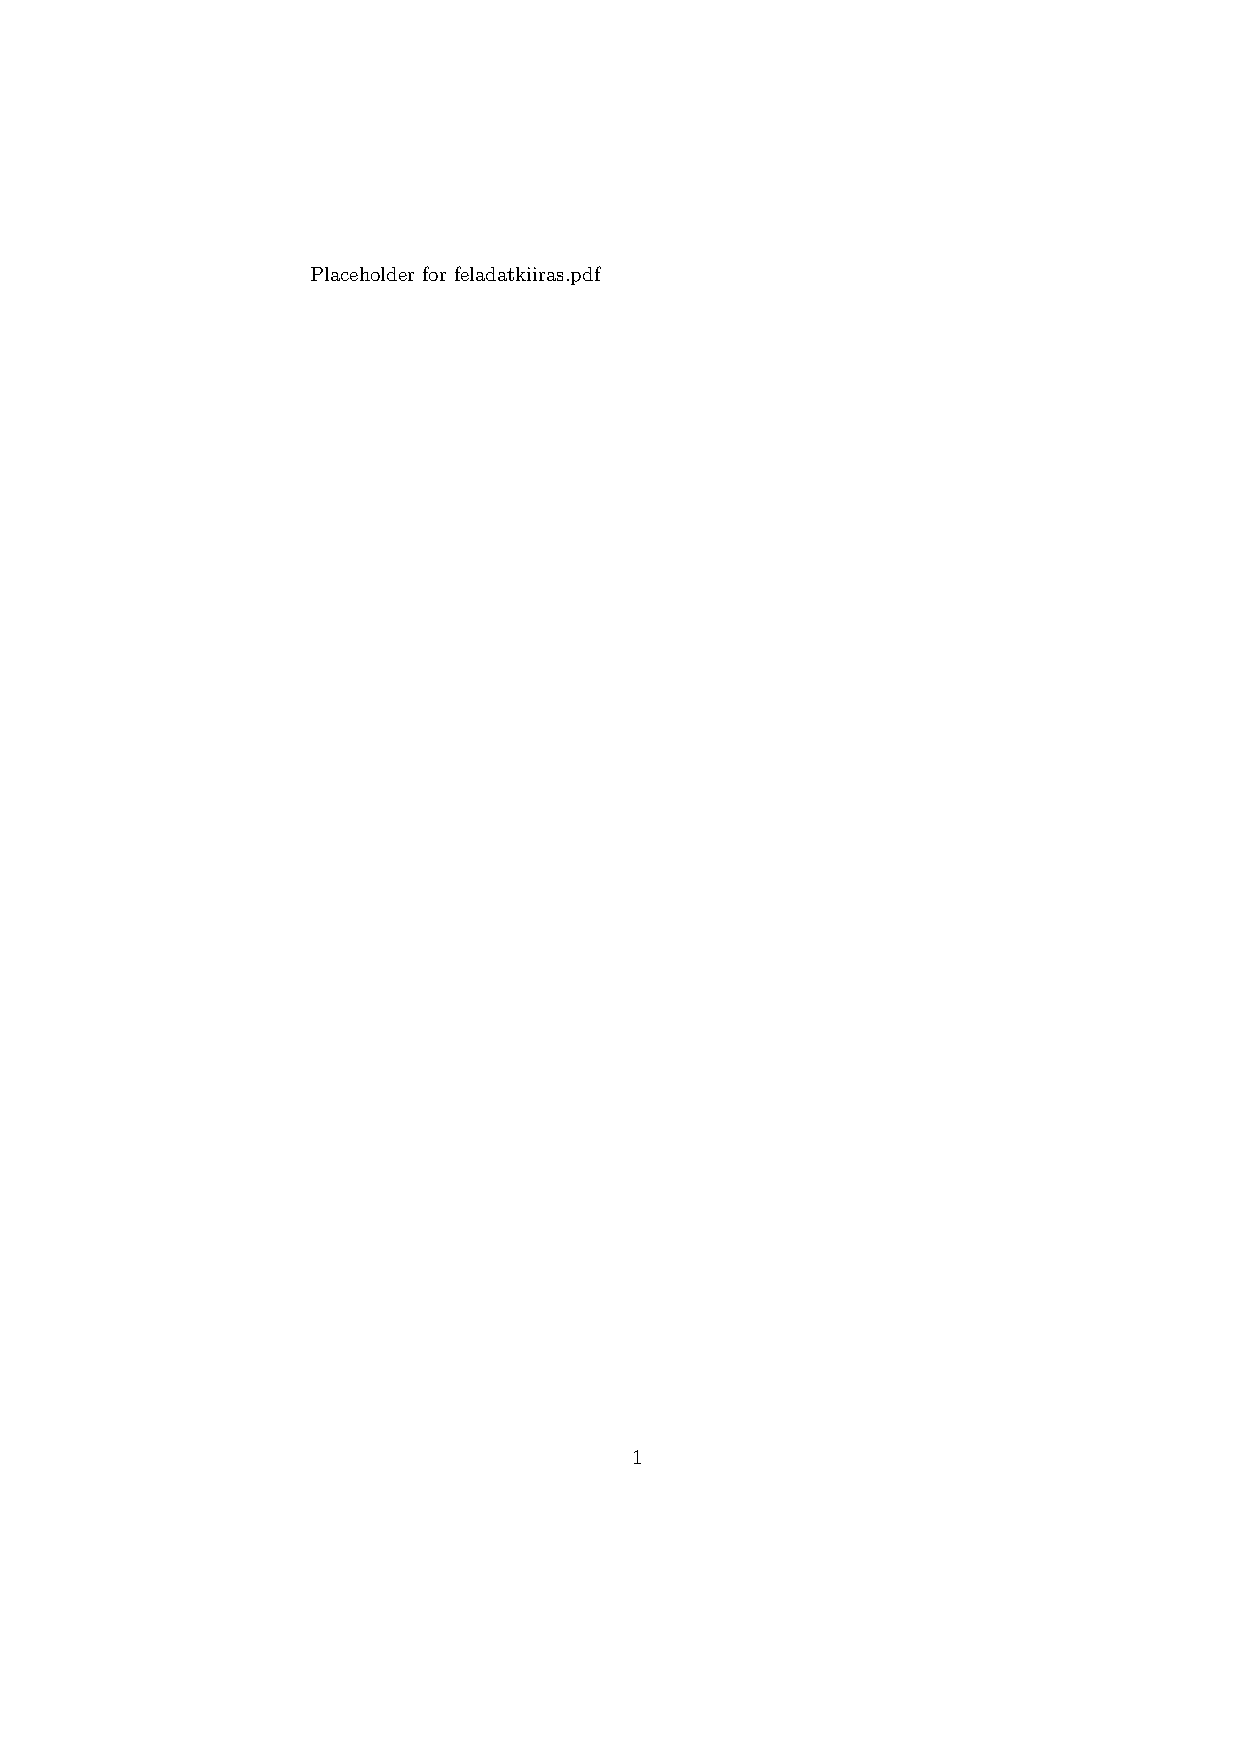
\includepdf[pages=1]{feladatkiiras.pdf}

% Nyilatkozatok [Declarations]
\selectlanguage{magyar}
\selecthungarian
\pagenumbering{roman}
\setcounter{page}{6}
\cleardoublepage % duplexnél páratlan oldalon legyen
%--------------------------------------------------------------------------------------
% Nyilatkozatok
%--------------------------------------------------------------------------------------
\begin{center}
\section*{NYILATKOZATOK}
\end{center}

\vspace{0.5cm}


%--------------------------------------------------------------------------------------

\begin{center}
\emph{Nyilatkozat az önálló munkáról}
\end{center}
Alulírott,  \emph{\authorFamilyName{} \authorGivenName} (\neptun), az Eötvös Loránd Tudományegyetem hallgatója, büntetőjogi és fegyelmi felelősségem tudatában kijelentem és sajátkezű aláírásommal igazolom, hogy ezt a \MakeLowercase{\munkatipustHU} meg nem engedett segítség nélkül, saját magam készítettem, és szakdolgozatomban csak a megadott forrásokat használtam fel. Minden olyan részt, melyet szó szerint vagy azonos értelemben, de átfogalmazva más forrásból átvettem, egyértelműen, a hatályos előírásoknak megfelelően, a forrás megadásával megjelöltem.

Ennek a szakdolgozatnak önálló, eredeti szerzője vagyok, ez az önálló szellemi alkotás jogtisztaság szempontjából megfelel az „Eötvös Loránd Tudományegyetem Szervezeti és Működési Szabályzata, II. kötet, Hallgatói Követelményrendszer. Módosításokkal egybeszerkesztett változat [2017. szeptember 1.]” c. szabályzat 74/A–74/C. §-aiban foglalt rendelkezéseknek.

\begin{flushleft}
Szombathely, \today
\end{flushleft}

\begin{flushright}
 \makebox[7cm]{\rule{6cm}{.4pt}}\\
 \makebox[7cm]{\emph{hallgató}}
\end{flushright}


\vfill
\clearpage

\selectthesislanguage

\newcounter{romanPage}
\setcounter{romanPage}{\value{page}}
\stepcounter{romanPage}


\selectthesislanguage
% Tartalomjegyzék [Table of Contents]
\setcounter{tocdepth}{3}  % Tartalomjegyzék mélysége [ToC depth]
\tableofcontents\vfill

% Ábrák és táblázatok jegyzéke [List of Figures, Tables]
%TODO Kommenteld ki, ha használni szeretnéd. [Uncomment to use]
%\listoffigures\addcontentsline{toc}{chapter}{\listfigurename}   % Ábrák jegyzéke - opcionális
%\listoftables\addcontentsline{toc}{chapter}{\listtablename}     % Táblázatok jegyzéke - opcionális

\chapter*{Előszó}\addcontentsline{toc}{chapter}{\eloszo}
Már a középiskolás éveim során érdeklődtem a 3D tervezés, a CAD-CAM világa felé. Gépi forgácsoló szakmámból kifolyólag elég régóta kürölvesz engem a gépészeti világ és akkor jött a gondolat, mi lenne ha jelentkeznék egyetemre. Életem egyik legjobb döntése volt a gépészmérnöki képzés elkezdése. Rengeteg új információval gazdagodtam, sokkal jobban el tudtam mélyülni a CAD-CAM rendszerekben, valamint megismerkedtem számomra addig teljesen ismeretlen módszerekkel. Az egyik ilyen volt a végeselem analízis. Ez a terület tetszett meg a legjobban a képzés során, rengeteg lehetőség rejlik benne. A szakdolgozati téma kiválasztásánál számomra fontos volt, hogy a CAD-CAM, valamint a végeselem analízis szerepet kapjanak az elkészítés során.


\begin{center}
    $\thicksim \; \thicksim \; \thicksim$
\end{center}


\subsubsection*{Köszönetnyilvánítás}
\emph{Elsőként szeretném megköszönni a TDK Hungary Components Kft.-nek, hogy a gépészmérnöki képzésem alatt biztosítottak számomra duális gyakorlati helyet, valamint hogy támogatták a szakdolgozatom minőségi elkészültét. Szeretném megköszönni az Eurosolid Zrt.-nek, hogy biztosították számomra a Soldiworks 2022 Student Edition CAD szoftvert, amellyel a modelleket készítettem el.}

\vspace{0.5cm}

\begin{flushleft}
{Szombathely, \today}
\end{flushleft}

\begin{flushright}
\emph{\authorName}
\end{flushright}
\vfill

\chapter*{Jelölések}\addcontentsline{toc}{chapter}{\jelolesek}
%----------------------------------------------------------------------------

A táblázatban a többször előforduló jelölések magyar és angol nyelvű elnevezése, 
valamint a fizikai mennyiségek esetén annak mértékegysége található. Az egyes 
mennyiségek jelölése – ahol lehetséges – megegyezik hazai és a nemzetközi 
szakirodalomban elfogadott jelölésekkel. A ritkán alkalmazott jelölések 
magyarázata első előfordulási helyüknél található.

%~~~~~~~~~~~~~~~~~~~~~~~~~~~~~~~~~~~~~~~~~~~~~~~~~~~~~~~~~~~~~~~~~~~~~~~~~~~~~~~~~~~~~
% A táblázatokat ABC rendben kell feltölteni, először mindig a kisbetűvel
% kezdve. Ha egyazon betűjelnek több értelmezése is van, akkor mindegyiket kü-
% lön sorban kell feltüntetni. Konstansok esetén az értéket is a táblázatba
% kell írni.
% Dimenzió nélküli mennyiségek mértékegysége 1 és nem: – !
% A jelölésjegyzékben csak SI vagy SI-n kívüli engedélyezett mértékegységeket
% szabad feltüntetni. Egy dokumentumon belül az SI és pl. az angolszász
% mértékrendszer nem keverhető!
%~~~~~~~~~~~~~~~~~~~~~~~~~~~~~~~~~~~~~~~~~~~~~~~~~~~~~~~~~~~~~~~~~~~~~~~~~~~~~~~~~~~~~

%~~~~~~~~~~~~~~~~~~~~~~~~~~~~~~~~~~~~~~~~~~~~~~~~~~~~~~~~~~~~~~~~~~~~~~~~~~~~~~~~~~~~~
% A Jelölés oszlop alapvetően kurzív betűváltozattal szedendő, a Mértékegység
% oszlopot álló betűkkel kell szedni. Felső indexhez használható a \tss{}
% parancs.
%~~~~~~~~~~~~~~~~~~~~~~~~~~~~~~~~~~~~~~~~~~~~~~~~~~~~~~~~~~~~~~~~~~~~~~~~~~~~~~~~~~~~~

\def\arraystretch{1.5}%  vertical cell padding

\subsubsection*{Latin betűk}
\begin{center}
    \begin{tabular}{lp{10cm}l}
        \hline
        Jelölés & Megnevezés, megjegyzés, érték & Mértékegység \\ 
        \hline
        $E$     & Rugalmassági modulusz  & GPa     \\
        $F$     & erő                        & N           \\
        $S$     & keresztmetszet             & mm\tss{2} \\
        \hline
    \end{tabular}    
\end{center}



\subsubsection*{Görög betűk}
\begin{center}
    \begin{tabular}{lp{10cm}l}
        \hline
        Jelölés & Megnevezés, megjegyzés, érték & Mértékegység \\ 
        \hline
                $\varepsilon$  & alakváltozás           & 1    \\
        $\sigma$  & feszültség                  & MPa             \\      

        \hline
    \end{tabular}
\end{center}



\subsubsection*{Indexek, kitevők}
\begin{center}
    \begin{tabular}{lp{12.8cm}}
        \hline
        Jelölés & Megnevezés, értelmezés\\ 
        \hline
        $e$     & elem  \\
        max     & maximális érték        \\
        \hline
    \end{tabular}    
\end{center}


\def\arraystretch{1}%  vertical cell padding

% Főszöveg [The main part of the thesis]
\cleardoublepage
\pagenumbering{arabic}
\chapter{Szakirodalmi áttekintés}
\section{Bevezetés}
Az anyagtudomány és mérnöki tervezés fő célja az, hogy megértsük az anyagok alapvető jellemzőit, mint a szilárdság, rugalmasság és törékenység. Ennek érdekében különféle mérő és értékelő módszereket alkalmazunk, hogy pontosan meghatározzuk ezeket a tulajdonságokat. A mérési folyamatok központi elemei a szakítópofák, amelyek elengedhetetlen eszközei az anyagok szakítószilárdságának vizsgálatának. A szakítószilárdság az a feszültség, amelyet az anyag képes elviselni anélkül, hogy eltörne. Ennek a tulajdonságnak az ismerete kulcsfontosságú az anyagok hatékony használatához és a termékek hosszú élettartamának biztosításához.

Ebben a szakdolgozatban a lapos próbatestekhez használt szakítópofák tervezési folyamatát mutatom be. A tervezés során számos szempontot kell figyelembe venni, többek között, hogy a pofa stabilan fogja a próbatestet, megakadályozza annak deformálódását, és egyenletes erőátvitelt biztosítson. A tervezett szakítópofa megfelelőségének ellenőrzésére végeselem-szimulációkat végzek, amik segítenek felmérni a tervezési paraméterek és az anyagok, valamint a geometriai formák kölcsönhatásait.

Végül bemutatom a szakítópofa gyártási folyamatát is. A gyártást úgy alakítottam ki, hogy maximalizáljam a termék minőségét és hatékonyságát, miközben minimalizálom a költségeket és az időt. A szakdolgozat célja, hogy hozzájáruljak a gyakorlati alkalmazások fejlesztéséhez, megbízható mérési eszközök létrehozásához, és az anyagok hatékony alkalmazásához.
\newpage

\section{Szakító próbatest}
A tervezés megkezdése előtt ismertetem az anyagvizsgálattal kapcsolatos alapismereteket.

A szakítóvizsgálat azon anyagvizsgálati módszerek közé tartozik, amelyeknél a mintát vagy próbatestet roncsolják és az ebből a roncsolásból származó eredményeket használják fel ahhoz, hogy megállapítsák az anyag mechanikai tulajdonságait. A szakítóvizsgálatnál a vizsgálandó darabból először egy szakító próbatestet készítenek, amely az erre vonatkozó szabványok szerint készül. Ez a próbatest többnyire lapos vagy hengeres. A szakdolgozat elkészítése során, a DIN 50125:2022 szabvány szerinti E formát használom (\ref{Fig:probatest}. ábra).

\begin{figure}[H]
\centering
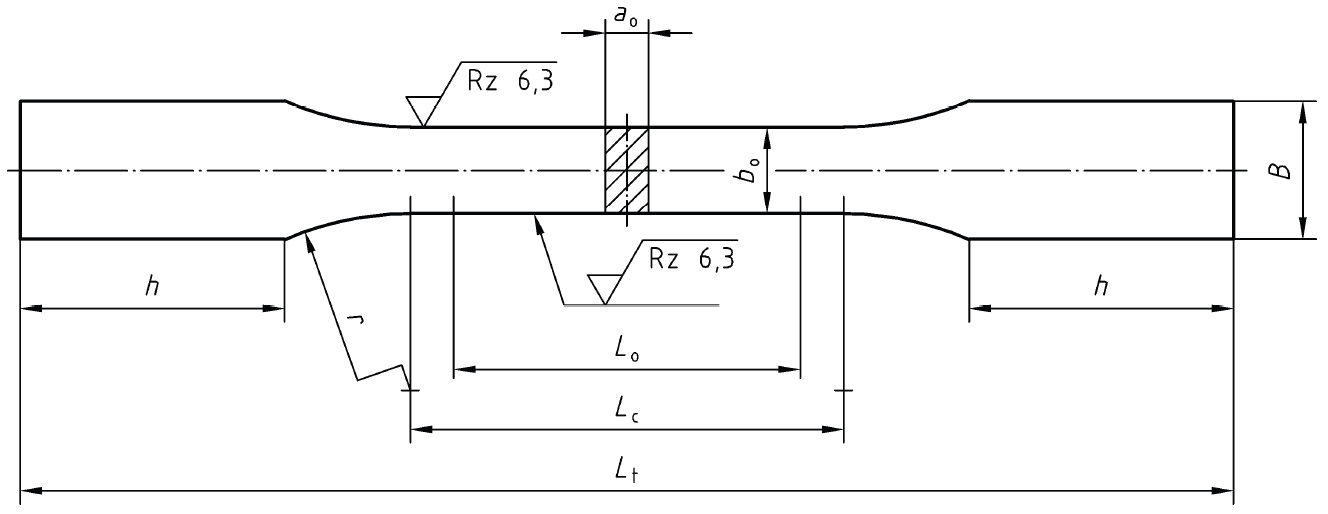
\includegraphics[width=15cm]{figures/probatest}
\caption{A szabvány szerinti próbatest}
\label{Fig:probatest}
\end{figure}
\noindent ahol:

\typeout{
\begin{center}
\begin{tabular}{l l l l}
$a_0$:	& Próbadarab vastagsága	& $L_0$:	& Kezdeti hossz ($L_0=5,65\sqrt{a_0\cdot b_0}$),	\\
$b_0$:	& Próbadarab szélessége, & $L_c$:	& Mérési hossz ($L_c\geq L_0+1,5\sqrt{a_0\cdot b_0}$),\\
$B$:	& Befogás szélessége ($\approx 1,2b_0+3\ mm$),	& $L_t$:	& Teljes hossz.	\\
$h$:	& Befogás hossza ($\approx 2b_0+10\ mm$),		&			&
\end{tabular}
\end{center}
}
\begin{itemize}
\item $a_0$: Próbadarab vastagsága,
\item $b_0$: Próbadarab szélessége,
\item $B$: Befogás szélessége ($\approx 1,2b_0+3\ mm$),
\item $h$: Befogás hossza ($\approx 2b_0+10\ mm$),
\item $L_0$: Kezdeti hossz ($L_0=5,65\sqrt{a_0\cdot b_0}$),
\item $L_c$: Mérési hossz ($L_c\geq L_0+1,5\sqrt{a_0\cdot b_0}$),
\item $L_t$: Teljes hossz
\item $r$: Lekerekítési sugár.
\end{itemize}
Ezeket a próbatesteket többféle méretben el lehet készíteni, attól függően, hogy mekkora alapanyag áll rendelkezésünkre. Ezek a méretek az \ref{Tab:probatest}. táblázatban találhatók.



\begin{table}[H]
\captionsetup{justification=raggedright,singlelinecheck=off}
\caption{A szakító próbatest méretei}
\vspace{-32pt}
\centering
\begin{flushright}
\begin{footnotesize}
A táblázatban szereplő értékek milliméterben
\end{footnotesize}
\end{flushright}
\vspace{-12pt}
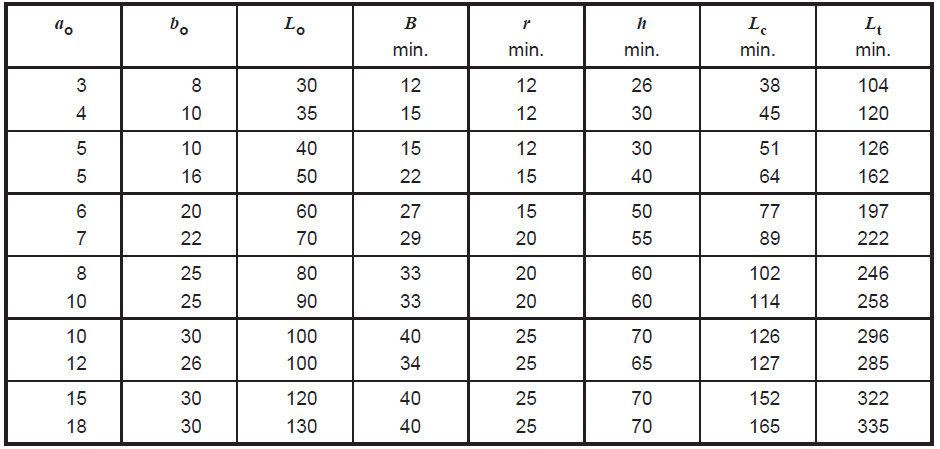
\includegraphics[width=15cm]{tables/probatest}
\label{Tab:probatest}
\end{table}

\section{Szakítóvizsgálat, szakítódiagram}
\noindent A feszültség és az alakváltozás közötti kapcsolatot gyakran egy grafikonon ábrázolják, amelyet szakítódiagramnak neveznek. Ezen a grafikonon láthatóak az anyag különböző mechanikai tulajdonságai:
\begin{itemize}
\item \textbf{Szakítószilárdság ($\sigma_U$):} Ez az a pont a grafikonon, ahol az anyag eléri a maximális feszültséget, mielőtt eltörik.
\item \textbf{Folyáshatár ($\sigma_Y$):} Az a feszültségszint, aminél az anyag megkezd egy jelentős, visszafordíthatatlan alakváltozást. Itt az anyag már nem rugalmasan, hanem plasztikusan deformálódik.
\item \textbf{Rugalmassági modulusz ($E$):} A rugalmas tartományban az alakváltozás és a feszültség közötti arány, amelyet a szakítódiagram kezdeti, egyenes szakaszának meredekségeként határoznak meg.
\end{itemize}

A vizsgálat után az anyag törési felületét is megvizsgálják. Ez többek között információval szolgál az anyag mikrostruktúrájáról, és segíthet meghatározni, hogy a törés plasztikus vagy rideg volt-e. Plasztikus törés esetén általában szemcsés, durva törési felület látható, míg rideg törésnél a felület simább és egyenletesebb.

A törés helye és a szakítódiagram adatai alapján további következtetéseket lehet levonni az anyag terhelés alatti viselkedéséről. Ez segíthet például abban, hogy milyen anyagokat érdemes használni bizonyos alkalmazásokban, ahol extrém terhelések lépnek fel \cite{pek2015anyag,lovas2011anyagismeret}.

\begin{figure}[H]
\begin{center}
\begin{tikzpicture}[scale=1.3]
\draw[thick,->] (0,0) -- (9,0) node[anchor=north] {$\varepsilon\ [-]$};
\draw[thick,->] (0,0) -- (0,7) node[anchor=east] {$\sigma\ [MPa]$};
\draw[very thick] (0,0) -- (1.5,4) -- (1.6,3.5) -- (1.65,3.8) -- (1.7,3.65) -- (1.72,3.75) -- (1.75,3.72) -- (1.8,3.75) -- (1.85,3.7) -- (1.9,3.75) -- (1.95,3.7) -- (2,3.75);
\draw[very thick] (2,3.75) to[out=80, in=180] (5,6) to[out=0, in=120] (7,5);
\draw[dashed] (0,6) -- (5,6);
\draw[dashed] (0,5) -- (7,5);
\draw[dashed] (0,4) -- (1.5,4);
\draw (-0.3,6) node {$\sigma_U$};
\draw (-0.3,5) node {$\sigma_F$};
\draw (-0.3,4) node {$\sigma_Y$};
\draw[dashed] (1.5,0) -- (1.5,4);
\draw[dashed] (2,0) -- (2,3.75);
\draw[dashed] (5,0) -- (5,6);
\draw[dashed] (7,0) -- (7,5);
\draw (0.8,-0.3) node {I.};
\draw (1.8,-0.3) node {II.};
\draw (3.5,-0.3) node {III.};
\draw (6,-0.3) node {IV.};
\draw[dashed] (1.25,0) arc (0:70:1.25);
\draw (0.6,0.4) node {$\alpha$};
\end{tikzpicture}
\caption{Lágyacél szakítódiagramja}
\label{Fig:Szakdiag}
\end{center}
\end{figure}

A szakítódiagram felosztható 4 részre az \ref{Fig:Szakdiag}. ábra szerint:
\begin{itemize}
\item I. szakasz: Elasztikus deformációs szakasz
\item II. szakasz: Kezdeti plasztikus deformációs szakasz
\item III. szakasz: Plasztikus szakasz
\item IV. szakasz: Kontrakciós szakasz
\end{itemize}

\subsection{I. szakasz}
Az \ref{Fig:Szakdiag}. ábra első szakaszában az anyag a húzás során rugalmasan deformálódik, ez azt jelenti, hogy ha itt megszakítanánk a vizsgálatot, akkor a próbatest visszanyerné eredeti alakját. Ezen a szakaszon tudjuk értelmezni a rugalmassági moduluszt ($E$), amely a mérnöki gyakorlatban alkalmazott anyagok egyik legjelentősebb tulajdonsága. A lineáris szakasz meredekségéből lehet kiszámítani az alábbi képlettel:
\pagebreak

\begin{equation}
E=\dfrac{\delta \sigma}{\delta \varepsilon}
\end{equation}
ahol:
\begin{itemize}
\item $E$: rugalmassági modulusz
\item $\delta \sigma$: feszültségváltozás [MPa]
\item $\delta \varepsilon$: fajlagos nyúlás változása
\end{itemize}

Másik lényeges anyagtulajdonság a deformációkból kiszámítható Poisson-tényező, amely a különböző irányokban mérhető deformációk között teremt kapcsolatot. Az extenzométer segítségével megmérhetjük a keresztirányú deformációt, amelyet a próbatest a húzás során elszenved. A térfogatmegmaradás törvénye miatt a vizsgálat során a próbatest hossza megnő, viszont ezzel egyidőben ezzel a nyúlással arányosan keresztirányú méretcsökkenésnek kell fellépnie.
\begin{equation}
\nu=-\dfrac{\varepsilon_x}{\varepsilon_z}=\dfrac{\delta w}{\delta l}\cdot\dfrac{l_0}{w_0}
\end{equation}
ahol:
\begin{itemize}
\item $\nu$: Poisson tényező
\item $\varepsilon_x$: fajlagos keresztirányú nyúlás
\item $\varepsilon_z$: fajlagos hosszirányú nyúlás
\item $\delta w$: szélességváltozás
\item $\delta l$: hosszváltozás
\item $l_0$: kezdeti hossz
\item $w_0$: kezdeti szélesség
\end{itemize}

\subsection{II. szakasz}
A második szakasz a kezdeti plasztikus szakasz, vagy közismertebb néven a megfolyás szakasza. Itt látszólag nem történik a próbatesten külső elváltozás. Ebben a szakaszban az anyag kristályrács szerkezete deformálódik és ez a szakítódiagramon tudjuk követni.

A kezdeti plasztikus szakaszban az anyag kristályrácsának atomjai vagy molekulái elmozdulnak egymáshoz képest, miközben kötések törhetnek vagy újra rendeződhetnek. Ez a deformáció mikroszkopikus szinten történik, és kis méretű plasztikus zónák jelennek meg az anyagban. Az anyag feszültségszintje ebben a szakaszban általában stabilizálódik, mivel az újonnan kialakuló kötések és a törött kötések közötti egyensúly kialakul.

A kezdeti plasztikus szakasz során az anyag tulajdonságai megváltoznak. Az anyag keménysége csökkenhet, míg a szilárdsága és a merevsége általában változatlan marad. Az anyag plasztikus deformációja során energia disszipálódik, és ez az energia leadódása hő formájában jelentkezhet.

A kezdeti plasztikus szakasz meghatározása fontos szerepet játszik az anyagok és szerkezetek tervezésében és elemzésében. A tervezés során figyelembe kell venni az anyag plasztikus deformációs tulajdonságait, hogy elkerüljük a túlzott deformációt, a szerkezetek károsodását vagy az anyagok szilárdsági határának túllépését.

Ennek a szakasznak az elején mérhető feszültséget, valamint ha nincs konkrét, jól látható folyási szakasz, akkor 0,2\% maradó alakváltozásnál mért feszültséget nevezzük folyáshatárnak ($R_{eH}$ vagy $\sigma_Y$) \cite{pek2015anyag}.

\subsection{III. szakasz}
Ebben a szakaszban a próbatesten akkora feszültség generálódik, hogy az anyag nem tud tovább elasztikusan deformálódni, továbbiakban plasztikusan deformálódik, ami azt eredményezi, hogy a próbatest belső szerkezetében történő elváltozásoknak köszönhetően az anyag elkezd felkeményedni.

Ebben a szakaszban az anyagban ébredő feszültség már nem lesz egyenesen arányos a deformációval, fokozatosan csökken a feszültségnek az alakváltozás szerinti deriváltja.

Ennek a szakasznak a végén érjük el a maximális feszültséget, amely a próbatestben ébredhet. Ezt a feszültséget hívjuk szakítószilárdságnak ($R_m$, vagy $\sigma_U$). A szakítószilárdságnak a mérnöki rendszerben történő kiszámítása az alábbi képlettel történik:
\begin{equation}
\sigma_U=\dfrac{F_{max}}{S_0}
\end{equation}
ahol:
\begin{itemize}
\item $\sigma_U$: szakítószilárdság
\item $F_{max}$: próbatestben ébredő legnagyobb húzóerő
\item $S_0$: kezdeti keresztmetszet
\end{itemize}


A mechanikai tervezés során nem a maximális feszültségre, hanem a folyáshatárra támaszkodunk. A folyáshatár az a feszültségérték, ameddig az anyag még képes visszanyerni eredeti geometriáját, és a terhelés megszűnése után nem maradnak maradandó deformációk. A tervezési számítások során a folyáshatárt tekintik mérvadónak, és a biztonságos működés érdekében bevezetik a biztonsági tényezőt, amely csökkenti a tervezési feszültséget, így minimalizálva a szerkezeti károsodást és az ezzel járó balesetek kockázatát \cite{pek2015anyag}.

\subsection{IV. szakasz}
Az \ref{Fig:Szakdiag}. ábrának az utolsó szakaszát hívjuk kontrakciós szakasznak. Ezen a szakaszon a próbatesten látványos keresztmetszeti elváltozások keletkeznek, a próbatest itt szenvedi el a legnagyobb szélességcsökkenést és ezzel egyidőben a legnagyobb hosszváltozást.

A mérnöki rendszerben készített szakítódiagramon itt jelentős feszültségcsökkenést lehet látni, mivel a kezdeti keresztmetszethez képest kisebb keresztmetszeten alkalmazzuk a húzóerőt.

A kontrakciós szakasz végén a törési feszültség ($\sigma_F$) értéke olvasható le a hosszá tartozó törési alakváltozással ($\varepsilon_F$) \cite{pek2015anyag}.

\begin{figure}[H]
\centering
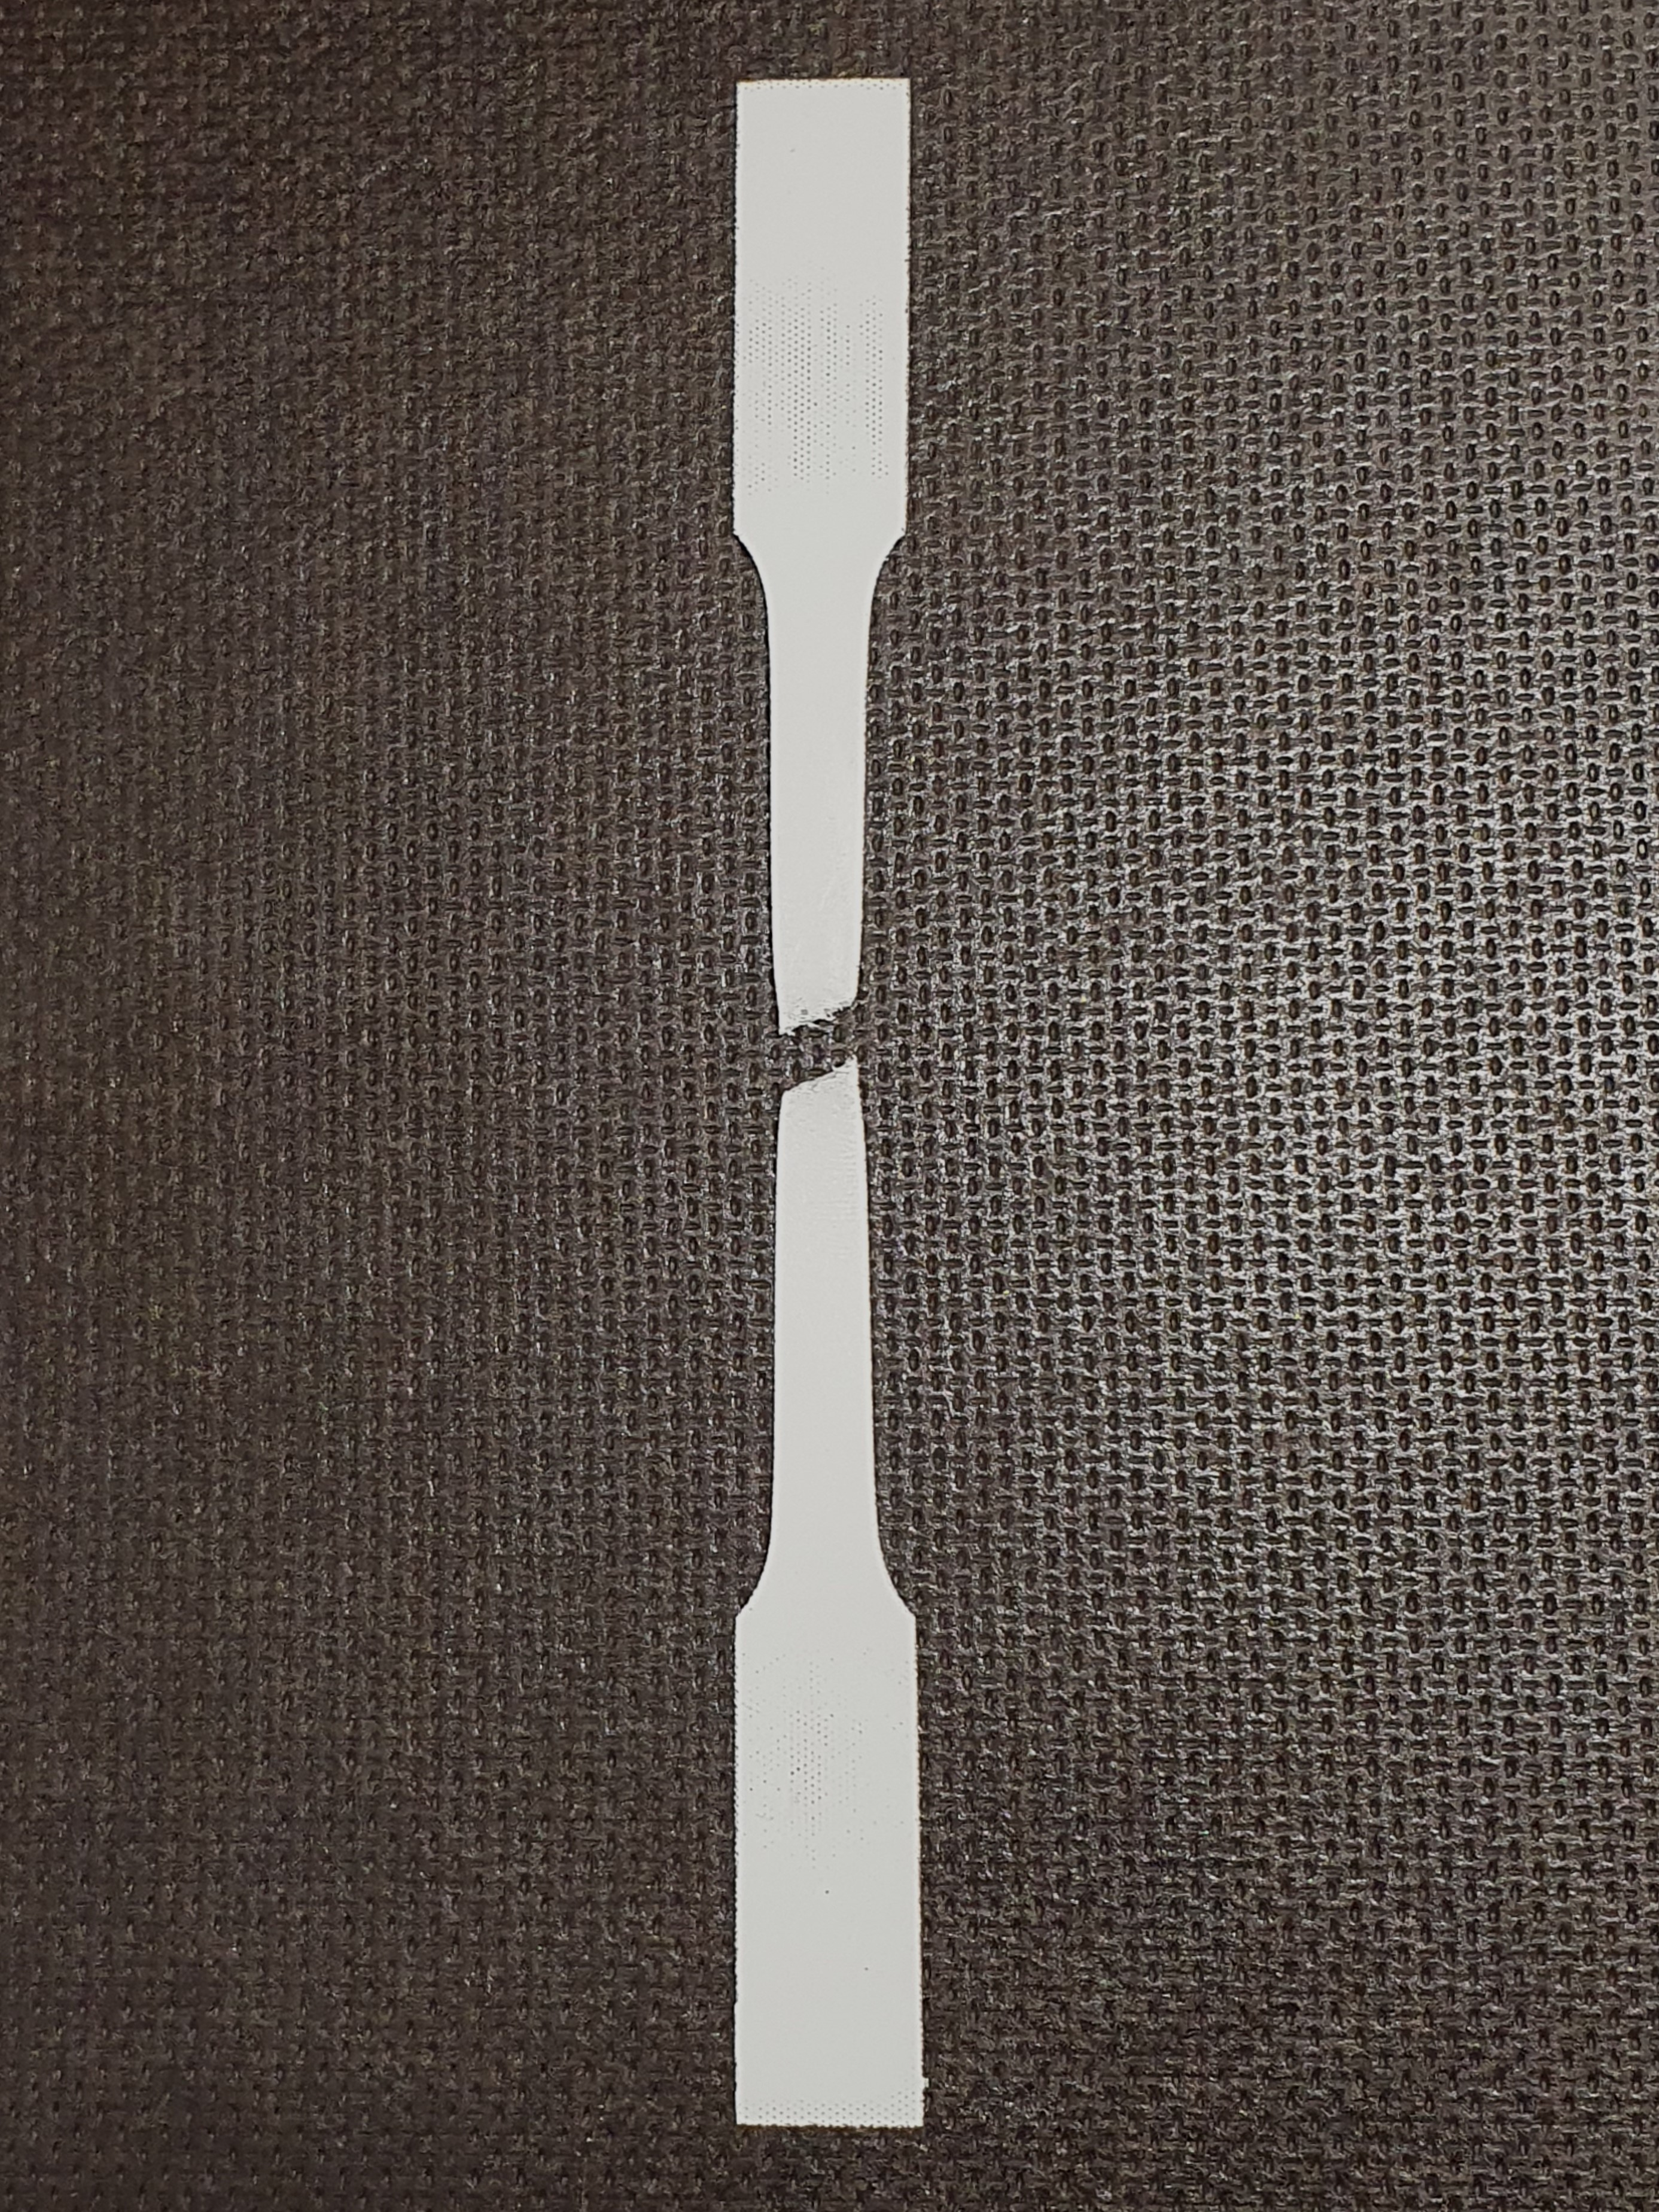
\includegraphics[width=8cm]{figures/probatest_eltort}
\caption{A laborban elszakított próbatest}
\label{Fig:probatest_eltort}
\end{figure}

\subsection{Szakítógép}
A szakdolgozat elkészítése során a laborban található Zwick Roell Z100 típusú univerzális szakítógépet, valamint annak megfogóit használtam. A Zwick Roell Z100 típusú szakítógép olyan univerzális anyagvizsgáló eszköz, amely széles körben alkalmazható a különböző anyagok tulajdonságainak tesztelésére. Képes meghatározni az anyagok szakítószilárdságát, nyúlását, rugalmassági moduluszát és egyéb mechanikai tulajdonságait. A különböző méretű és formájú próbatestekkel végzett vizsgálatok során a gép húzó, nyomó, hajlító és csavaró erőhatásokat képes alkalmazni. Így a gép az anyagok reakcióját az ezekre a terhelésekre mérve, képes meghatározni az anyagok viselkedését és tulajdonságait.
100 kN-os terhelhetőséggel rendelkezik, ami azt jelenti, hogy nagyfokú terhelési képességgel bír, így képes megbirkózni a legkülönfélébb anyagok, beleértve a kemény fémek és kompozit anyagok vizsgálatával is.

\begin{figure}[H]
\centering
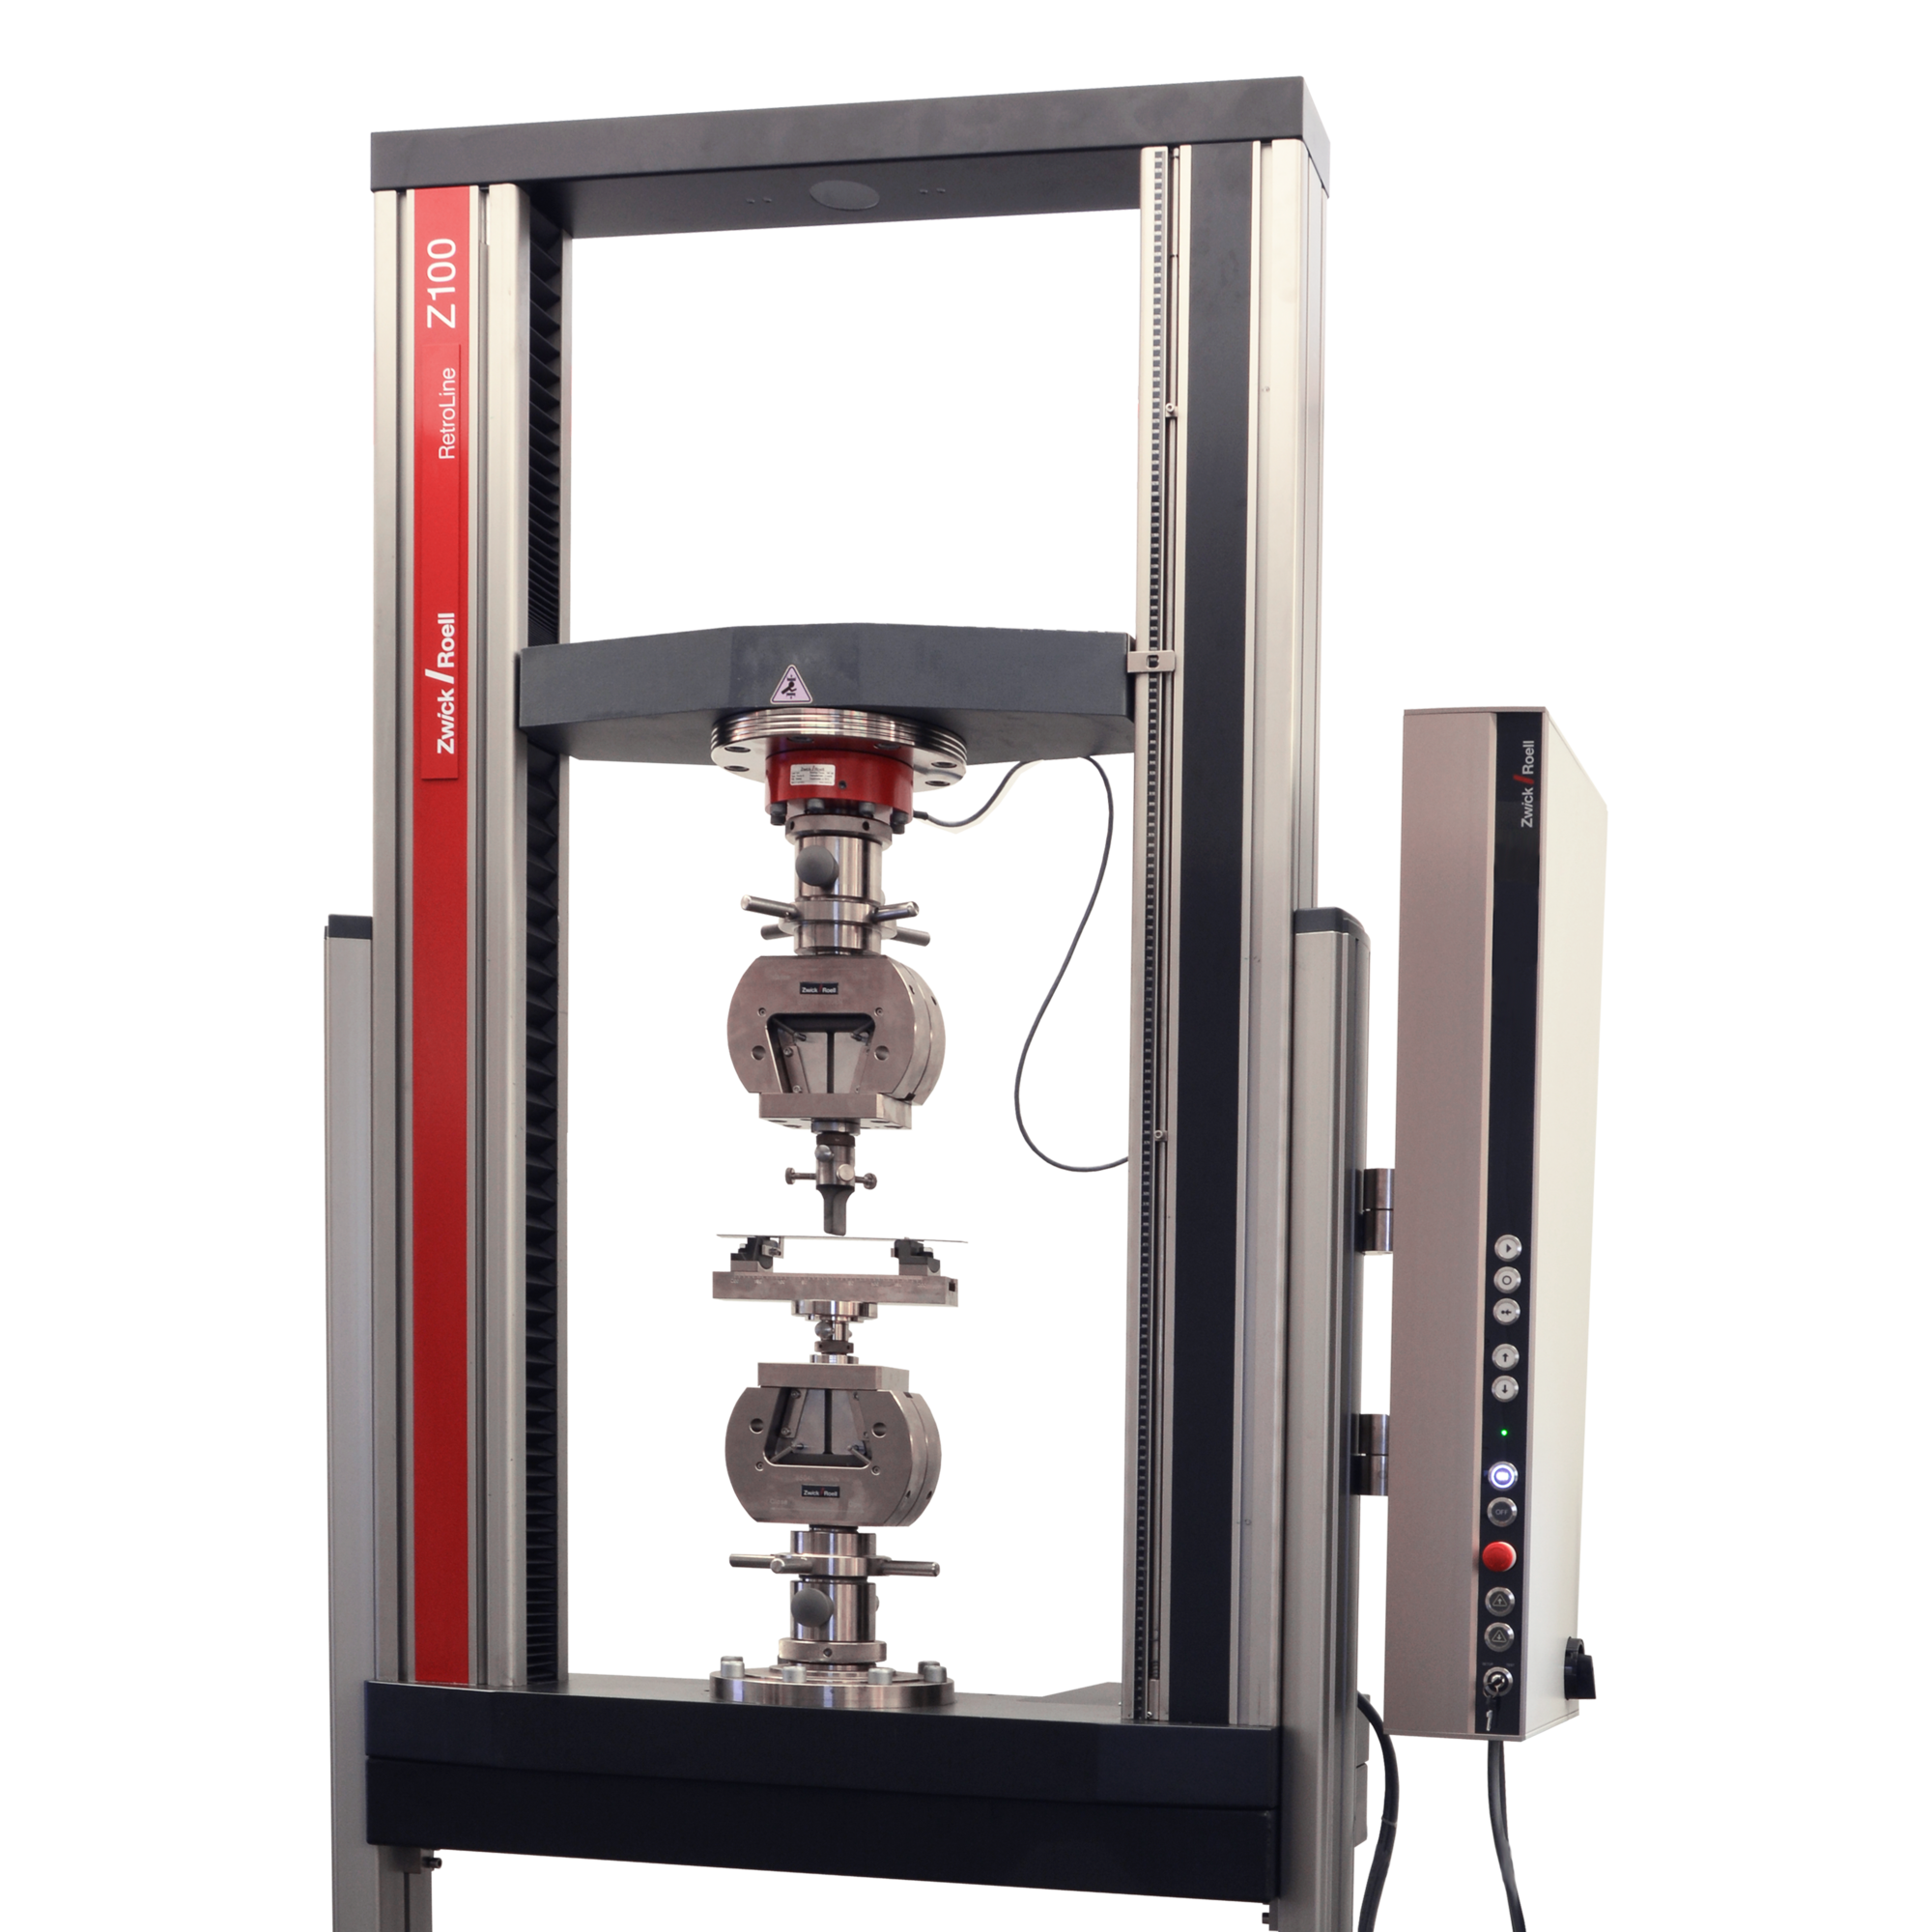
\includegraphics[width=14cm]{figures/zrz100}
\caption{A laborban használt szakítógép}
\label{Fig:zrz100}
\end{figure}

\subsection{Jelenlegi szakítópofa}
A szakítógépen a gyárilag kapható prizmás próbatest megfogó fej található, amely mechanikai úton szorítja össze a próbatestet. Kialakítása egyszerű, a cserélhető pofa egy prizmával érintkezik a fejhez, amelyet egy menettel tudjuk mozgatni és ez a mozgás szorítja össze a pofákat szimmetrikusan.

\begin{figure}[H]
\centering
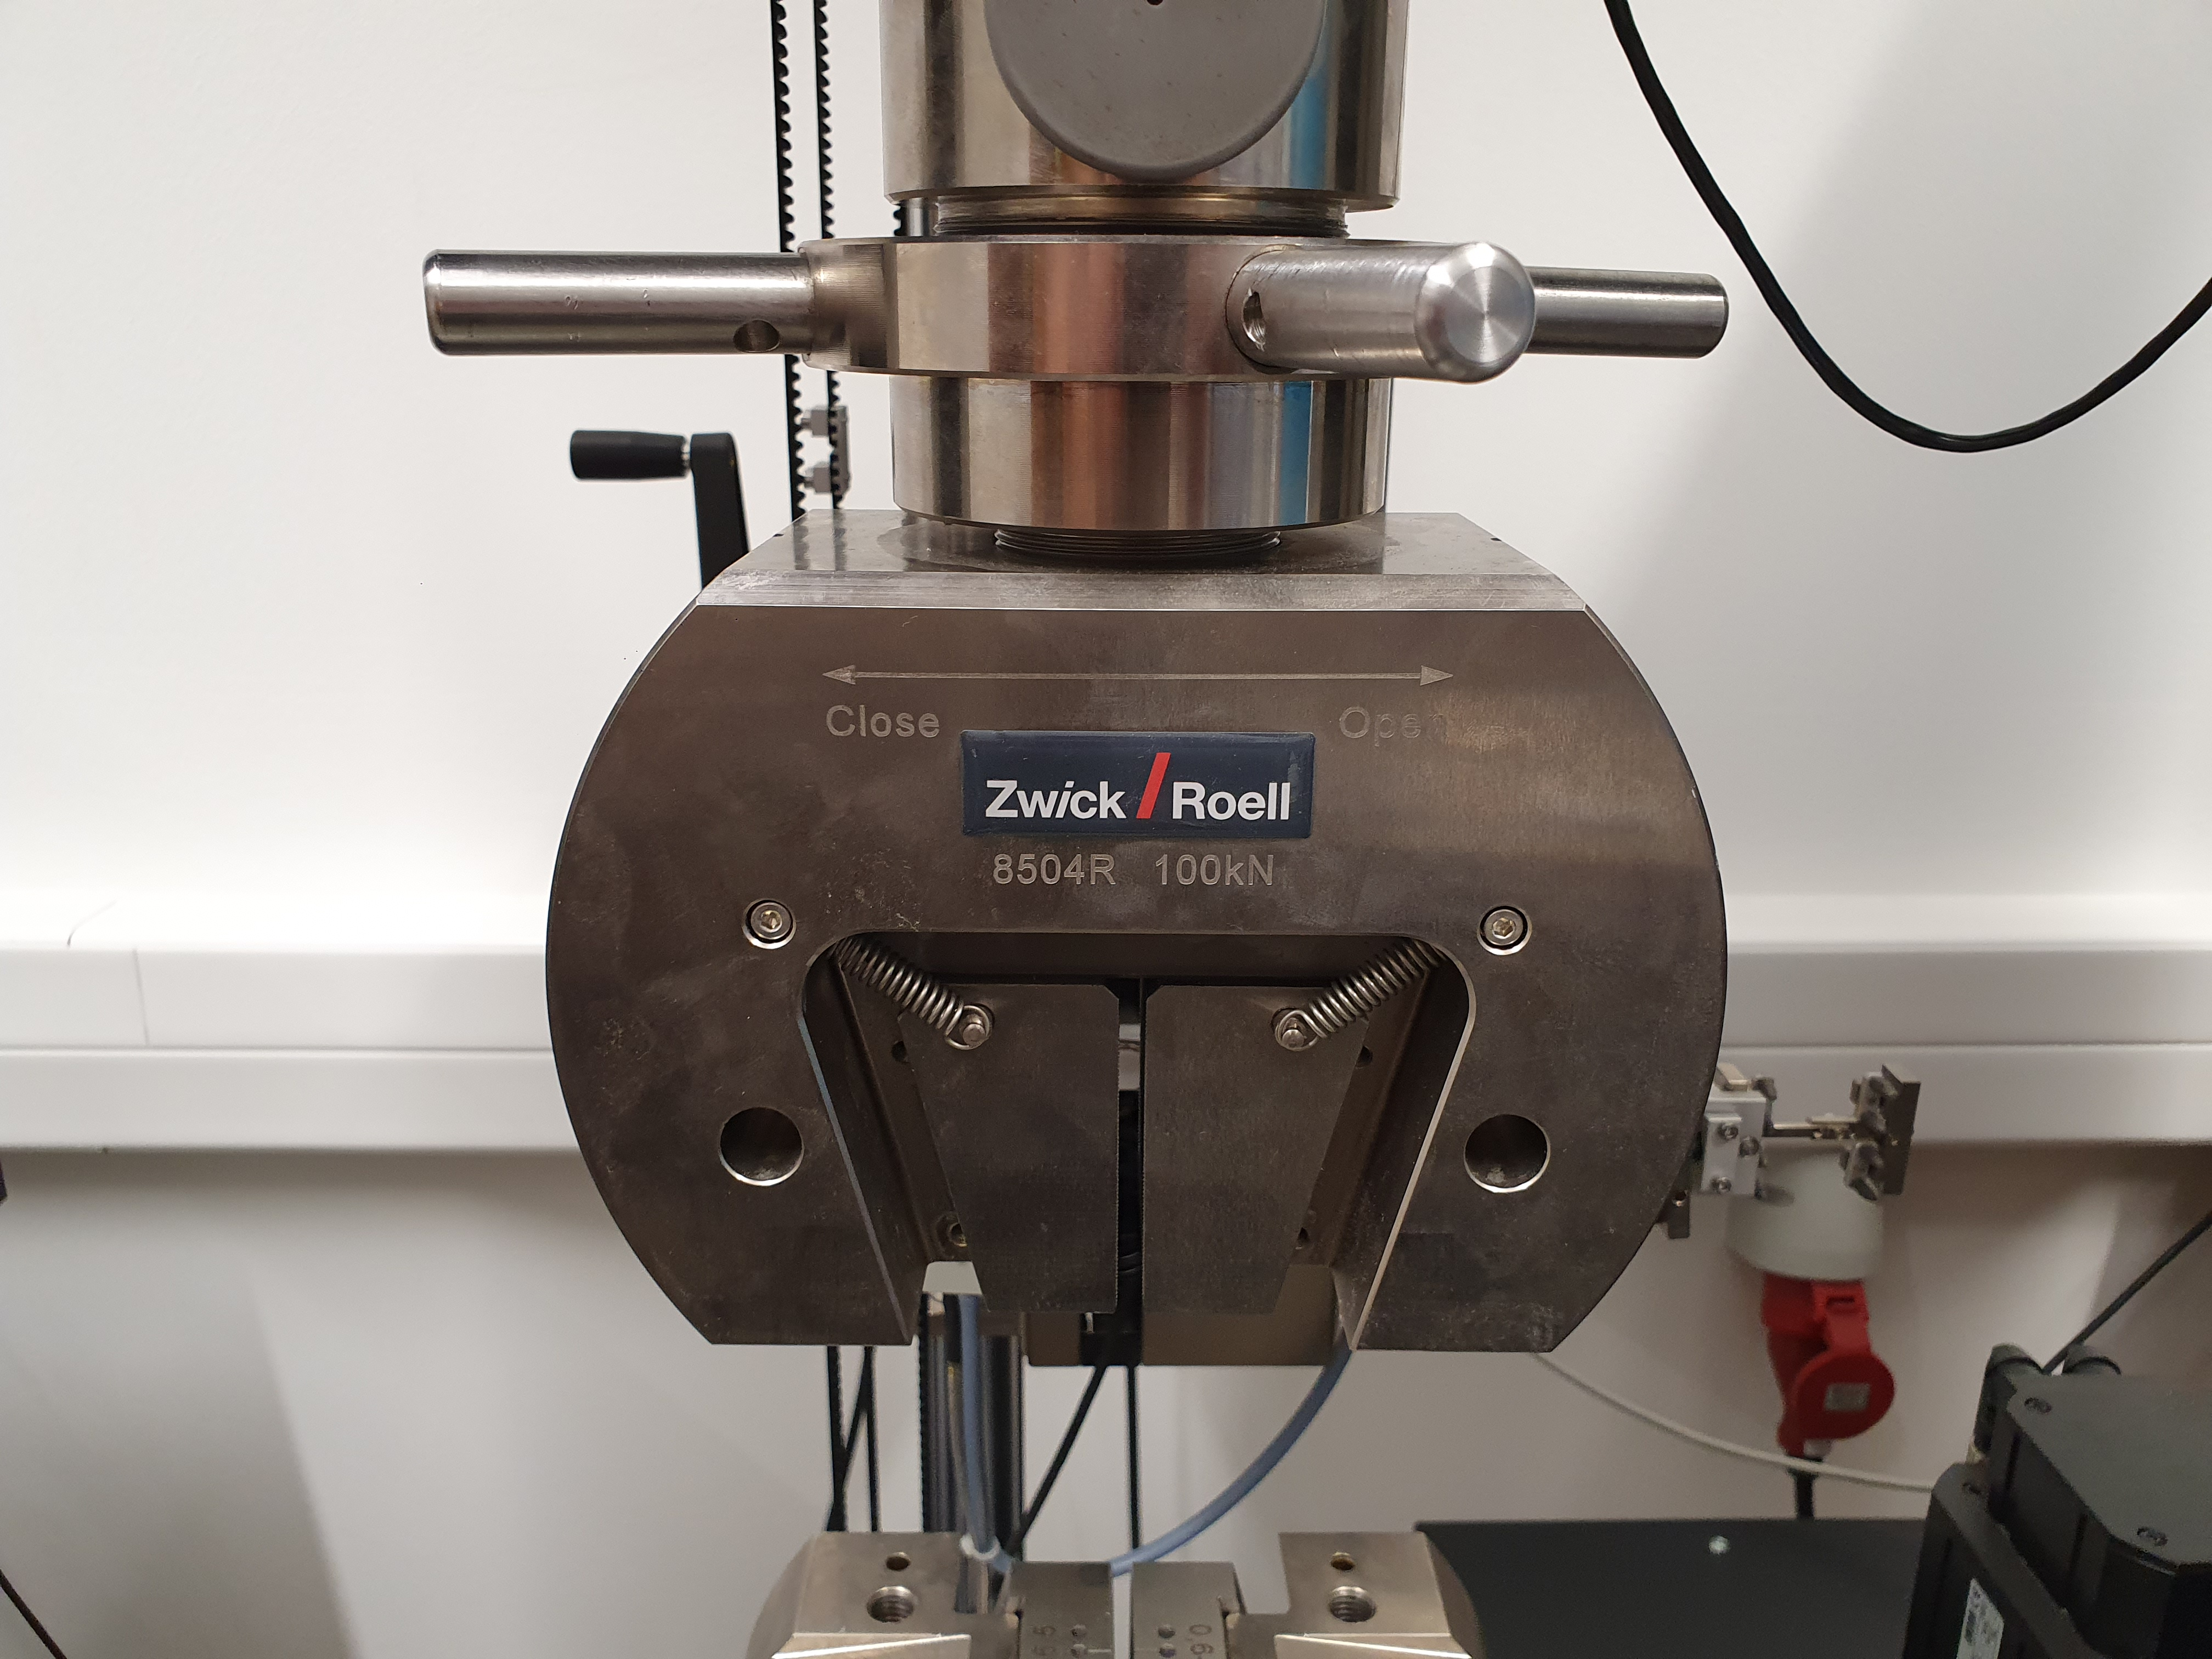
\includegraphics[width=12cm]{figures/fej}
\caption{A szakítógépre felszerelt fej}
\label{Fig:fej}
\end{figure}

\begin{figure}[H]
\centering
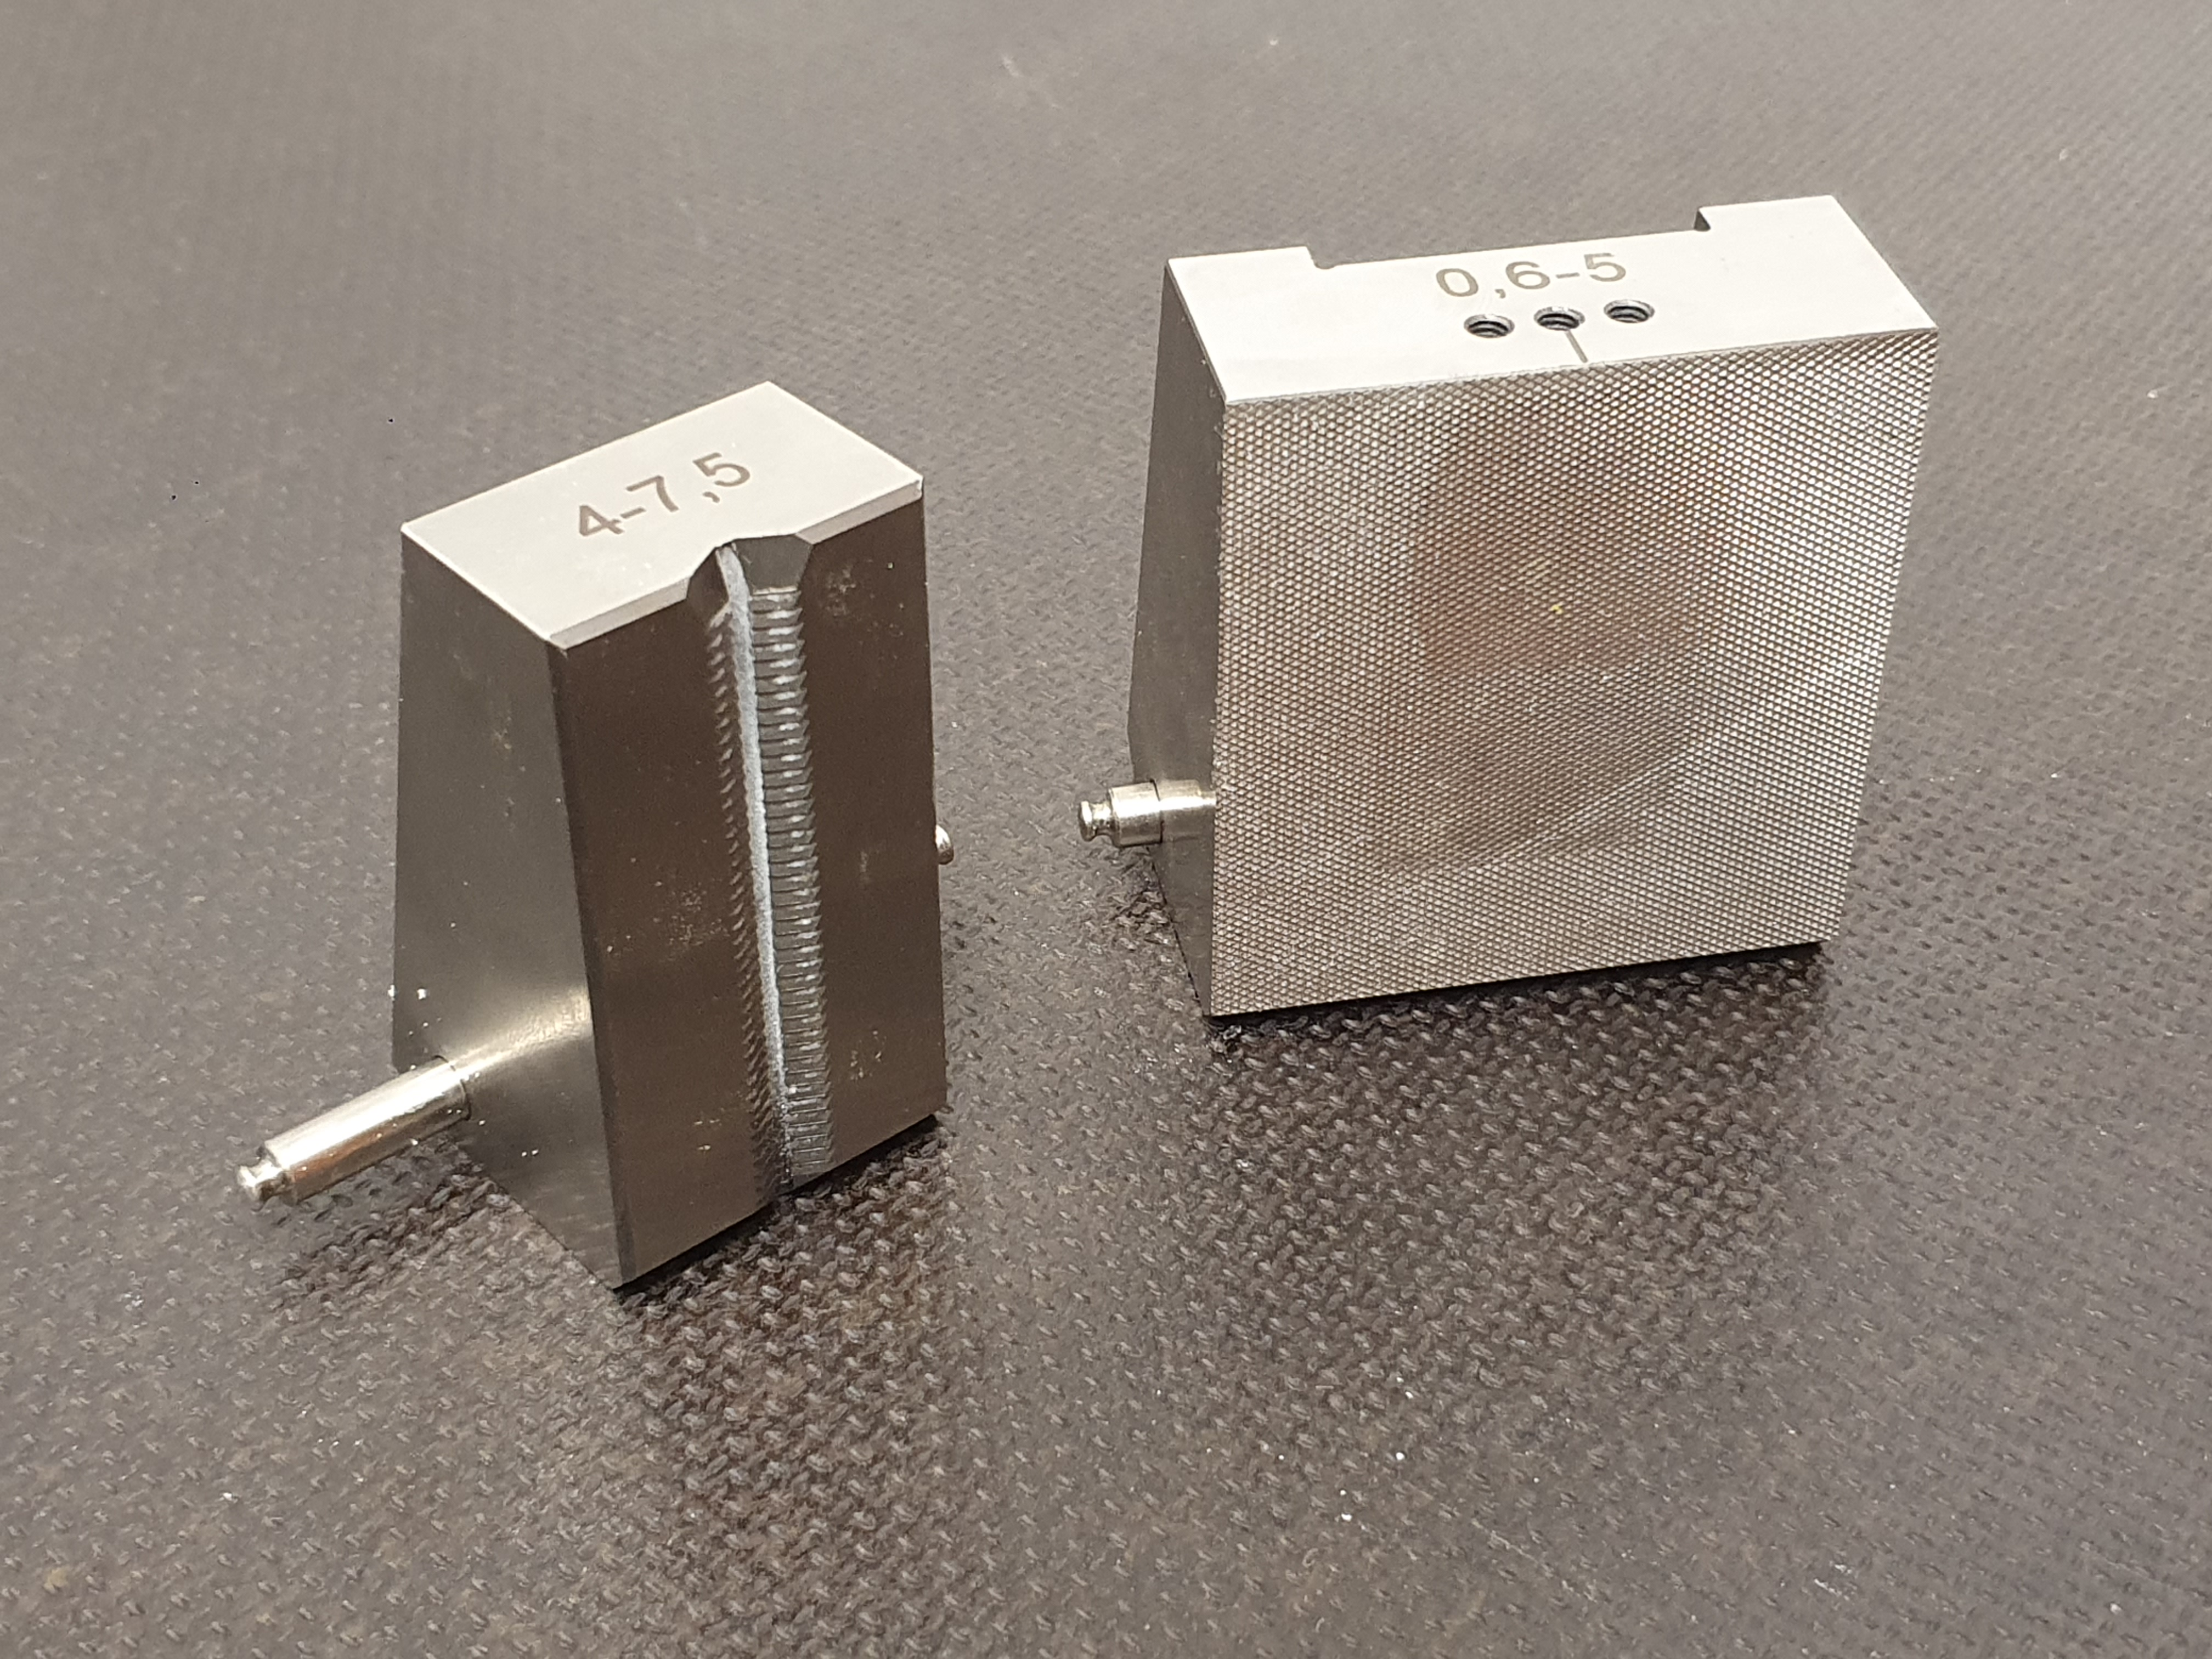
\includegraphics[width=12cm]{figures/pofak}
\caption{Bal oldalon a hengeres, jobb oldalon a lapos próbatestekhez készült pofa}
\label{Fig:pofak}
\end{figure}


%\begin{figure}[H]
%\centering
%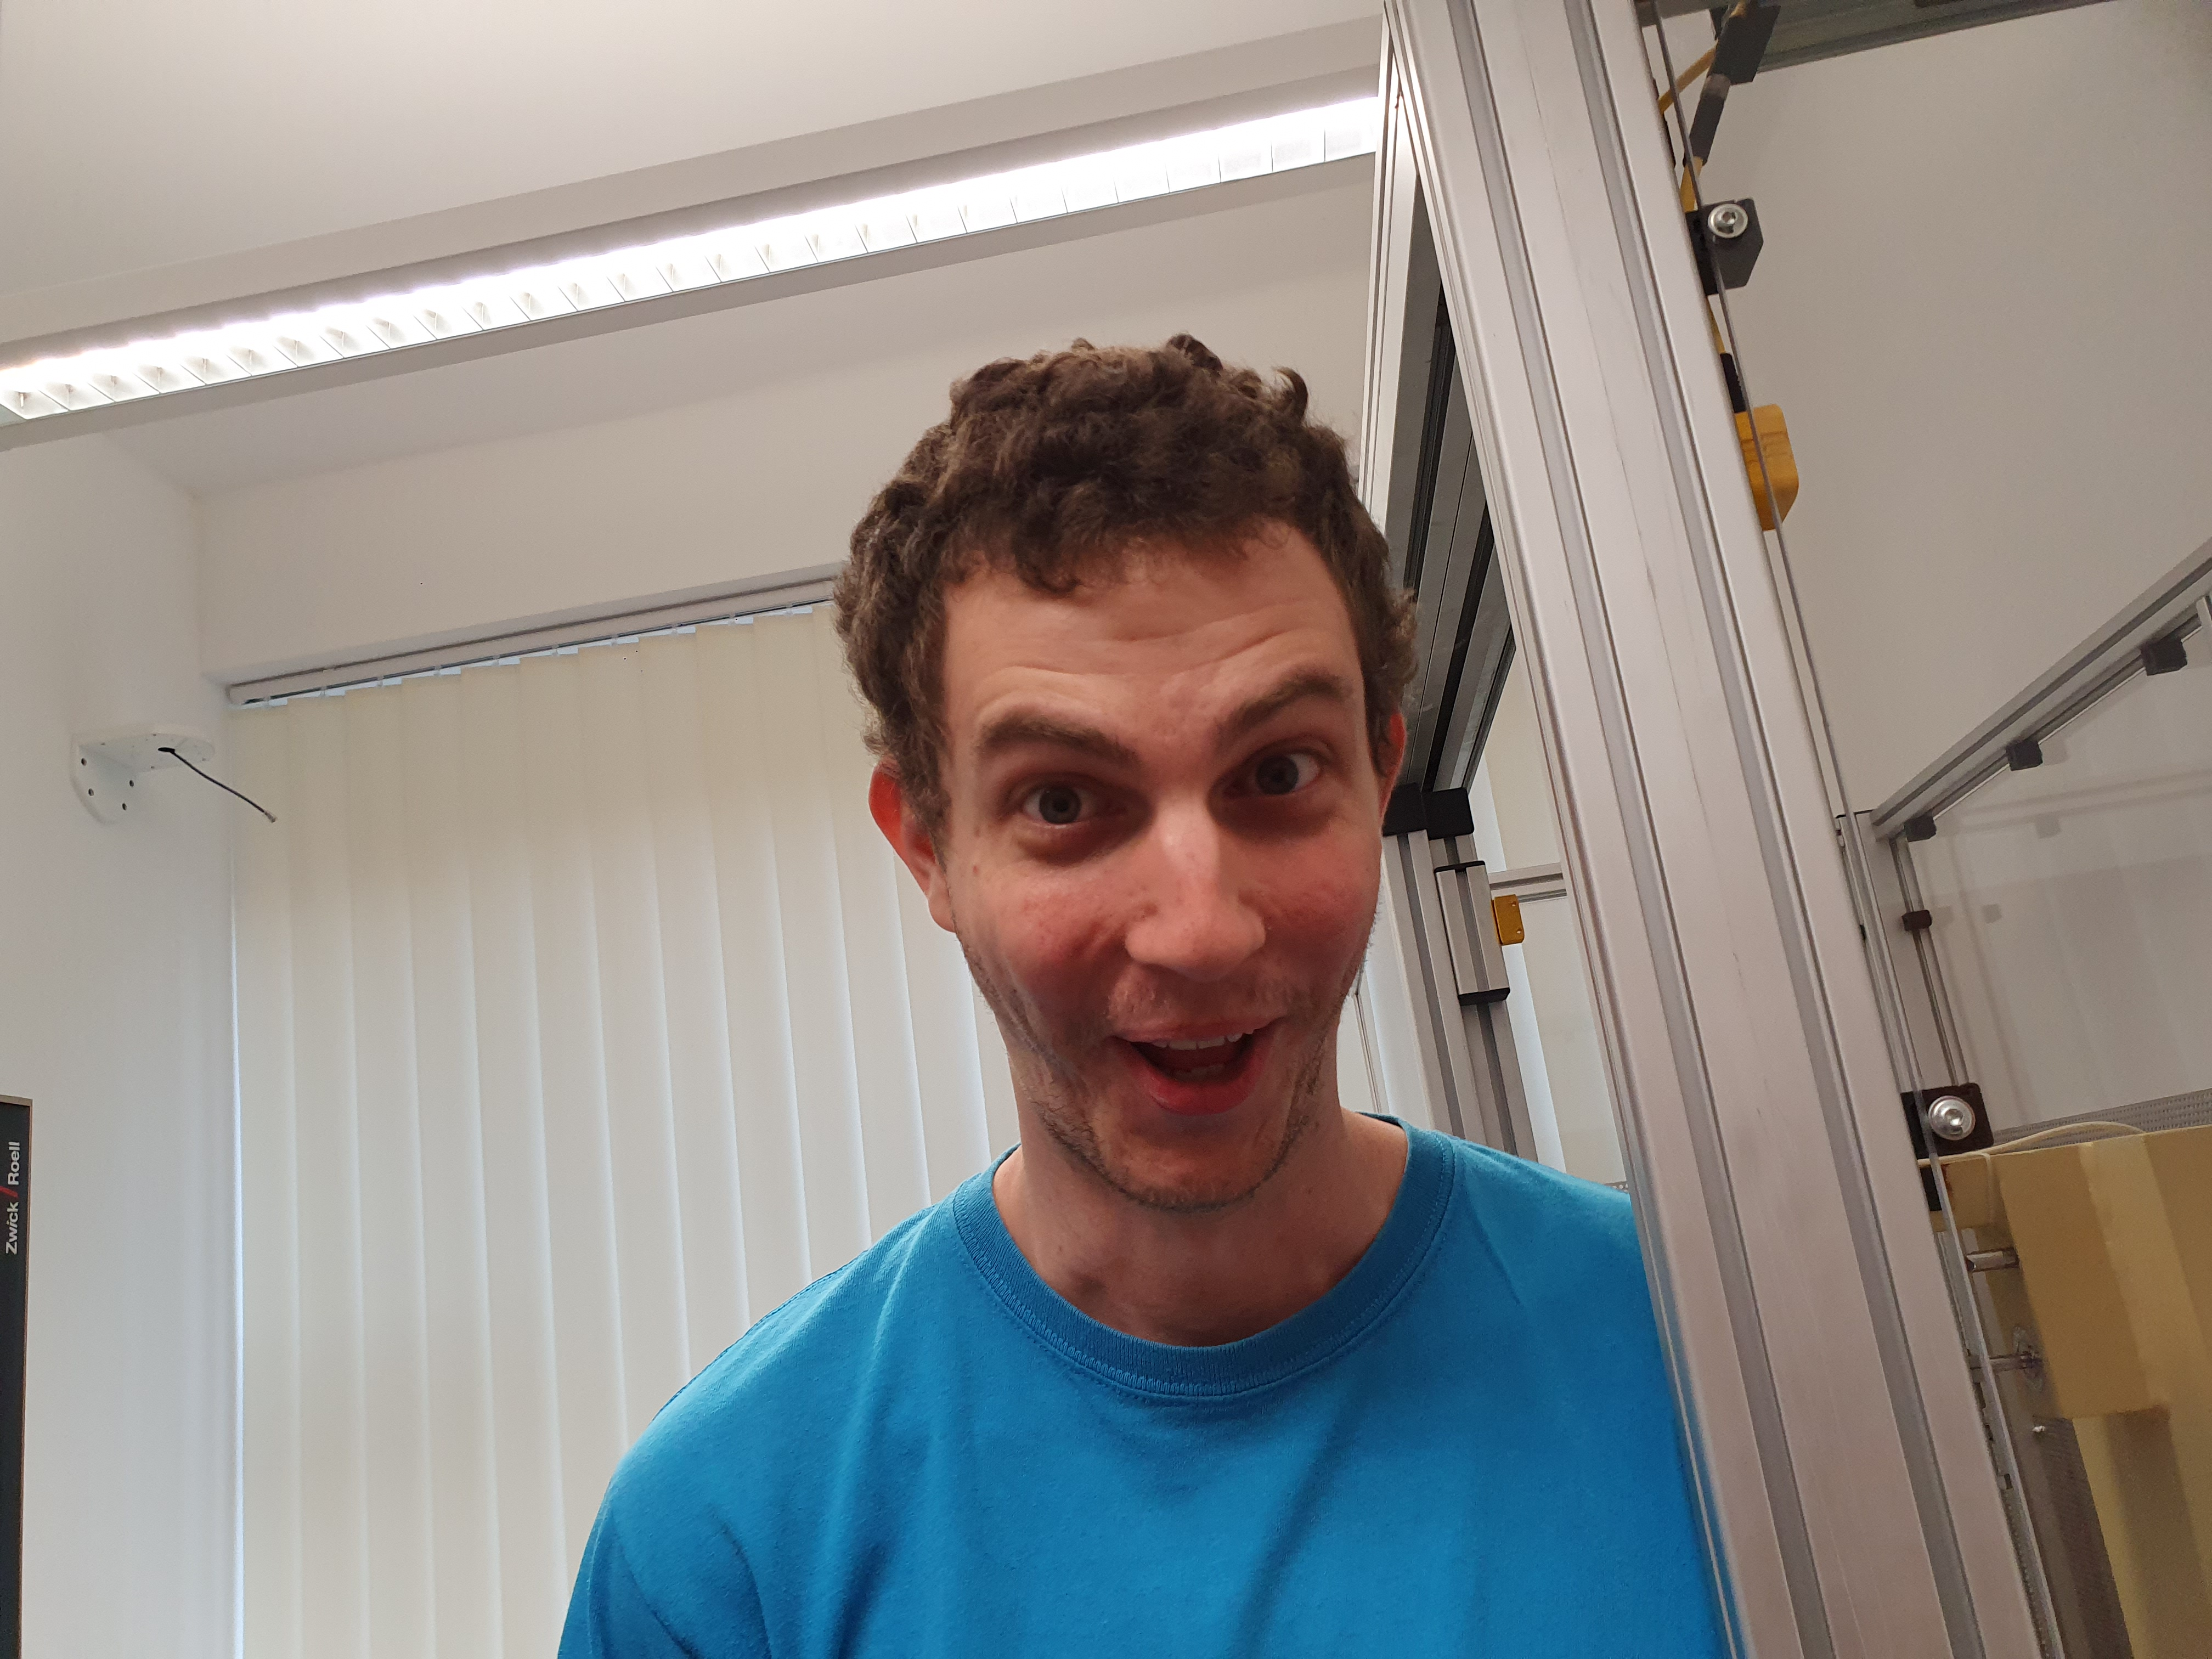
\includegraphics[width=14cm]{figures/bilosz}
%\caption{Bilosz Málton, PhD. hallgató}
%\label{Fig:bilosz}
%\end{figure}

\section{Végeselem analízis}
\subsection{A végeselem-analízis jelentősége}
A végeselem-módszer (Finite Element Method, FEM) az egyik legdinamikusabban fejlődő numerikus módszer, amely alapjaiban változtatta meg a mérnöki tervezés világát. A módszer gyökerei az 1940-es évekig nyúlnak vissza, amikor matematikusok és mérnökök olyan hatékony eszközök fejlesztésén dolgoztak, amelyek képesek a bonyolult geometriájú és viselkedésű szerkezetek viselkedésének előrejelzésére. Ma a FEM az egyik legelterjedtebb számítógépes modellezési technika, melynek segítségével a mérnökök képesek a szerkezeti és folyamatmérnöki problémák komplex analízisére és megoldására.

A módszer előnye abban rejlik, hogy képes a valóságosan bonyolult, nemlineáris szerkezeti viselkedést hitelesen modellezni, anélkül hogy drága és időigényes fizikai prototípusokat kellene készíteni. A FEM lehetővé teszi a terhelési állapotok, feszültségek és alakváltozások részletes elemzését már a tervezés korai szakaszában. Ennek köszönhetően csökkenthető a hibás konstrukciók száma, optimalizálható az anyagfelhasználás, és jelentős költségmegtakarítás érhető el, mindeközben növelve a termék biztonságát és megbízhatóságát. Az elmúlt évtizedekben a FEM fejlődése párhuzamosan haladt a számítástechnikai képességek rohamos növekedésével, lehetővé téve egyre részletesebb és komplexebb modellek készítését és elemzését.

Az ipari gyakorlatban a FEM ma már nélkülözhetetlen eszköz a gépészmérnökök számára, mivel lehetőséget nyújt a szerkezetek teljesítményének előrejelzésére, a tervezési hibák korai azonosítására, és az optimalizálásra, ami kiemelkedően fontos a versenyképes és innovatív termékek fejlesztése szempontjából. A FEM használatával a tervezési folyamat sokkal rugalmasabb és hatékonyabb, amely pozitív hatással van a mérnöki munka minden aspektusára \citep{molnarka2002matematikai, IEEEFEM2023}.

\typeout{\subsection{Alkalmazása a szakítópofa tervezésében}
A szakítópofák kulcsfontosságú szerepet töltenek be a mechanikai tesztelésben, ahol a próbatestek szakítószilárdságának meghatározása történik. A tervezés során fontos figyelembe venni a szakítópofára ható terheléseket, beleértve a maximális húzó-, nyomó- és oldalirányú terheléseket, valamint az ezekből eredő feszültségeket és alakváltozásokat. A terhelések ismerete nélkülözhetetlen a szakítópofa megbízhatóságának és funkcionalitásának biztosításához.
A végeselem-analízis (FEM) kritikus eszköz a szakítópofa tervezésének és fejlesztésének minden fázisában. Az anyagválasztás tekintetében a FEM lehetővé teszi a különféle anyagok viselkedésének szimulációját a tervezett terhelések alatt, segítve ezzel a legmegfelelőbb anyagok kiválasztását. Az analízis segítségével képesek vagyunk előre meghatározni azokat a kritikus pontokat, ahol esetleges anyagfáradás vagy törés várható, lehetővé téve az anyagösszetétel vagy a geometria módosítását.
A szakítópofa geometriai kialakításának optimalizálása is létfontosságú. A FEM alkalmazásával megvizsgálhatjuk a pofa különböző geometriai formáinak hatását a feszültségeloszlásra és az alakváltozásra, így a tervezés során már a gyártás előtt ki tudjuk javítani azokat a tervezési hibákat, amelyek meghosszabbíthatnák a kísérletek idejét vagy csökkenthetnék a mérési pontosságot.
Ezen felül, a szerkezeti megerősítések tervezésében is nagy szerepe van a FEM-nek. A szakítópofa kritikus pontjain ahol a legnagyobb terhelések jelentkeznek, a szerkezeti elemzések segítségével meghatározható, hogy hol szükséges megerősítéseket elhelyezni a biztonság és stabilitás növelése érdekében. A megerősítések helyének és méretének optimalizálásával a FEM hozzájárul a szerkezet teljes élettartamának és megbízhatóságának javításához.}

\subsection{Célja a szakdolgozat keretein belül}
A szakdolgozat keretein belül a végeselem-analízis (FEM) célja egy részletes és megbízható modell létrehozása a szakítópofa tervezéséhez, mely képes a kritikus terhelési pontok, a maximális feszültségek és alakváltozások pontos azonosítására. Ez a részletes elemzés lehetővé teszi a tervezési folyamat során fellépő potenciális gyenge pontok feltárását, és segít a szerkezeti megbízhatóság javításában a törési mechanizmusok és anyagfáradás megértésén keresztül.

A modell alapjául szolgáló adatok és feltételek tisztázása után a szakdolgozat kiemelten foglalkozik a tervezett szakítópofa szerkezeti reakcióinak vizsgálatával standard és extrém terhelési esetekre vonatkozóan. Cél, hogy a szakdolgozatban bemutatott elemzés eredményeképpen egy olyan tervezési prototípus jöjjön létre, amely megfelel a biztonsági és működési előírásoknak, miközben optimalizált az anyaghasználat és a gyártási költségek tekintetében is.

Az analízis során használt szoftver kiválasztásánál több szempontot is figyelembe kell venni: a szoftver elterjedtségét, a rendelkezésre álló modulokat és elemeket, a felhasználói felületet, valamint az adott szoftver által nyújtott analízis pontosságát és részletességét. A szakdolgozatban használt szoftver kiválasztását a fent említett szempontok mellett az egyetemi kurzusokon és a szakmai gyakorlat során szerzett tapasztalatok, valamint az iparági elfogadottság is befolyásolja. E szempontok fényében a választás egy olyan szoftverre esett, amelyik megfelelő kompromisszumot nyújt az analízis komplexitása és a felhasználói felület között, biztosítva ezzel a hatékony és precíz munkavégzést a szakdolgozat elkészítése során.

\section{Alapfogalmak és elméleti háttér}
A következőkben szeretnék kitérni a végeselem analízis témakörébe tartozó alapfogalmakra és a végeselem analízis elméleti hátterére. A fejezetben kitérek az alapvető elméletére, a merevségi mátrixra, a hálózásra, az anyagmodellekre, valamint a kezdeti- és peremfeltételekre.
\subsection{Alapvető elméleti koncepciók}
\textbf{Az energiaelv és a virtuális munka elve:}
\begin{itemize}
    \item \textbf{Az energiaelv:} Ezt az elvet arra használjuk, hogy megállapítsuk egy rendszer mechanikai állapotát, ahol az energia minimalizálása hozza létre az egyensúlyi állapotot. A potenciális energia minimális értéke az egyensúlyi konfigurációban fog megjelenni, ami alapvető a végeselem-módszerben történő modellezéskor.
    \item \textbf{A virtuális munka elve:} Egy másik alapvető koncepció, amely az anyagokon és szerkezeteken belüli belső erők és a külső terhelések közötti egyensúlyt írja le virtuális elmozdulásokon keresztül. Ezt az elvet arra használjuk, hogy a külső terhelések által végzett virtuális munka egyenlő legyen a belső erők által végzett virtuális munkával \cite{voros2012veges,pere2011vem}.
\end{itemize}
\newpage

\subsection{Merevségi mátrix}
A végeselem-analízis egyik kulcsfontosságú fogalma a merevségi mátrix, amely az egyes elemek merevségét reprezentálja és az egész szerkezet viselkedését határozza meg. Az egyes elemek merevségi mátrixait úgy tervezzük meg és aggregáljuk össze, hogy azok a globális szerkezeti modellt hozzák létre. Ez a globális mátrix tartalmazza az összes elemre vonatkozó merevségi információkat és lehetővé teszi, hogy a szerkezet teljes válaszát meghatározzuk a terhelések alatt.

A lokális merevségi mátrixok minden egyes végeselem számára külön-külön kerülnek meghatározásra, figyelembe véve az adott elem anyagi tulajdonságait, méreteit és a szerkezet geometriai viszonyait. Ezeket a lokális mátrixokat azután összeállítjuk egy globális merevségi mátrixba, amely a teljes szerkezet merevségi viszonyait írja le. Az aggregáció során figyelembe vesszük az elemek közötti csatlakozási pontokat és a határfeltételeket is.

A merevségi mátrix kialakítása a virtuális munka elvére és az energia megőrzésének elvére épül. Ez azt jelenti, hogy a szerkezet deformációjakor felhalmozódó belső rugalmas energia egyenlő a külső terhelések által végzett munkával. A virtuális munka elvének alkalmazásával a szerkezet egyensúlyi állapotát úgy írhatjuk le, hogy a virtuális elmozdulások esetén a belső és külső erők virtuális munkája nulla.

A merevségi mátrix fontos szerepet játszik abban, hogy modellezni tudjuk a szerkezeti elemek közötti kölcsönhatásokat. A mátrix elemei közvetlenül tükrözik az elemi csomópontok közötti merevségi kapcsolatokat, amelyek meghatározzák, hogyan oszlanak meg és terjednek el a belső erők és nyomatékok a szerkezeten belül. Ezáltal a merevségi mátrix nem csak az egyes elemek, hanem az elemek közötti kölcsönhatások viselkedését is leírja, lehetővé téve az analízis során a komplex terhelési állapotok pontos előrejelzését.

A merevségi mátrix létrehozása matematikailag a lokális elemi merevségi mátrixok egyesítésével történik, amelyeket a globális koordinátarendszerbe transzformálnak. Az alábbiakban egy egyszerűsített formában mutatom be a merevségi mátrix egy elemre vonatkozó képletét és a globális merevségi mátrixra való összeállítását. A merevségi mátrix $[K]$ az egyes elemek $D$ deformációs energiajának deriváltjaként jön létre a nodális elmozdulások u függvényében:
\begin{equation}
    [K] = \dfrac{\partial^2 D}{\partial u^2}
\end{equation}
ahol:
\begin{itemize}
    \item $[K]$: a merevségi mátrix,
    \item $D$: az elem deformációs energiája,
    \item $u$: a csomóponti elmozdulások vektora.
\end{itemize}

Egy konkrét elem $e$ merevségi mátrixát a következő képlet adja meg, ahol $E$ a rugalmassági modulus, $A$ az elem keresztmetszeti területe, $L$ az elem hossza, és az integrálást az elem hossza mentén végzik:
\begin{equation}
    [K^{(e)}] = \frac{E A}{L}
    \begin{bmatrix}
        1   &   -1 \\
        -1  &   1 
    \end{bmatrix}
\end{equation}

Az egész szerkezetre vonatkozó globális merevségi mátrix a következőképpen áll össze az egyes elemek lokális merevségi mátrixainak összeállításával és a megfelelő csomópontokhoz való hozzárendeléssel:

\begin{equation}
    [K_{\text{global}}] = \sum_{e=1}^{n} [T^{(e)}]^\top [K^{(e)}] [T^{(e)}]
\end{equation}
itt:
\begin{itemize}
    \item $[K^{(e)}]$: az $e$-edik elem lokális merevségi mátrixa,
    \item $[T^{(e)}]$: a transzformációs mátrix, ami az $e$-edik elem lokális koordinátáit transzformálja a globális koordinátarendszerbe,
    \item $n$ az elemek száma a szerkezetben.
\end{itemize}

A transzformációs mátrixok és a globális koordinátarendszerbe történő integrálás biztosítja, hogy minden elem merevségi jellemzői megfelelően szerepeljenek a teljes szerkezet merevségi viselkedésének modellezésében \citep{voros2012veges,paczelt2007veges,VEM2011}.

\subsection{Hálózás}
A hálózás a végeselem-analízis (FEM) egyik alappillére, hiszen a komplex geometriai formák és szerkezeti problémák számítását a véges elemekre való felosztás teszi lehetővé. A háló esszenciálisan egy digitális rács, ami a fizikai testet kisebb, kezelhető elemekre, úgynevezett véges elemekre bontja le. Ezen elemek közötti kapcsolatok és kölcsönhatások modellezik a teljes szerkezet viselkedését a valóságban jelentkező terhelések és környezeti hatások alatt.

A hálózás során az a cél, hogy a modell geometriáját és a szerkezeti viselkedését lehető legpontosabban leképezzük, miközben gazdaságosak maradunk a számítási erőforrásokkal. A háló kialakítása során olyan döntéseket kell meghozni, amelyek befolyásolják az analízis pontosságát és hatékonyságát, mint például az elemek mérete, alakja és eloszlása. Az ideális háló finoman követi a geometriai kontúrokat, elkerülve a túl nagy vagy túl kis elemeket, amelyek torzíthatják az eredményeket vagy feleslegesen növelik a számítási igényeket.

A háló minőségének biztosítása elengedhetetlen a megbízható FEM eredményekhez. Ha a háló nem megfelelően van felosztva, pontatlan eredményeket adhat, és ezen felül számítási hibákhoz is vezethet. Ebből adódóan, a hálózás nem egyszerűen a modell részekre történő bontása, hanem kritikus lépés a szerkezeti elemzésben, amely megalapozza a további analízis pontosságát és érvényességét.

A lineáris és kvadratikus elemek kiválasztása során figyelembe kell venni a vizsgálati célt, a rendelkezésre álló számítási erőforrásokat, valamint a kívánt pontosság és felbontás egyensúlyát. A kvadratikus elemek alkalmazása ajánlott ott, ahol az eredmények nagy pontossága elengedhetetlen, különösen ott, ahol a szerkezeti viselkedésben nemlineáris vagy nagyfokú geometriai változások vannak. Az ilyen elemek használata növelheti a számítási időt, de csökkentheti a szükséges elemek összmennyiségét a hálóban, optimalizálva ezzel a számítások gazdaságosságát. A lineáris elemek egyszerűbb esetekben, ahol a pontosság kevésbé kritikus, gyors és hatékony megoldást nyújthatnak. Az adaptív hálózati stratégiák segítségével tovább finomítható a háló a szükséges pontosság és számítási hatékonyság elérése érdekében \cite{tamas2014vegeselem}.

\subsection{Anyagtulajdonságok és anyagmodellek}
Az anyagtulajdonságok megfelelő meghatározása létfontosságú a végeselem-analízisben, hiszen ezek a paraméterek határozzák meg, hogy a szimulált szerkezeti elemek hogyan reagálnak a terhelésekre. A szakítópofák esetében különösen fontos, hogy az anyagtulajdonságok pontosan tükrözzék a valós viselkedést, mivel ezek a szerkezeti komponensek gyakran kerülnek maximális terhelés alá a vizsgálatok során.

\textbf{Rugalmassági modulus $(E)$:} Az anyag merevségét jellemzi, és azt fejezi ki, hogy az anyag mennyire ellenáll az alakváltozásnak. Nagyobb modulus esetén az anyag kevésbé deformálódik azonos feszültség hatására.

\textbf{Poisson-tényező $(\nu)$:} Ez az arányossági tényező leírja az anyag hosszanti megnyúlása és a keresztirányú összehúzódása közötti viszonyt.

\textbf{Szakítószilárdság $(\sigma_u)$:} Az a maximális feszültség, amit az anyag elvisel törés nélkül. Ez egy kritikus paraméter a törési analízisben.

Az anyagmodell kiválasztása a vizsgálandó jelenségektől függ. Ha az anyag viselkedése a vizsgált terhelési tartományban lineárisan rugalmas, akkor egy lineáris rugalmas modell alkalmazása elegendő. Itt az anyag viselkedése a Hooke-törvény által leírt módon lineáris, azaz az anyagban ébredő feszültség arányos az alakváltozással. Ebben az esetben az anyagmodell csak a rugalmassági modulust és a Poisson-tényezőt foglalja magában.

Elasztikus-plasztikus modellek alkalmazása akkor szükséges, ha az anyag átlépi a rugalmas tartományát és plasztikus alakváltozást szenved. Ezen modellek paramétereit sokkal összetettebb kalibrálni, mert figyelembe kell venni a folyáshatárt, a keményedési tulajdonságokat és a törési viselkedést is.

A modellek paramétereinek kalibrálása során kísérleti adatokra vagy megbízható szakirodalmi forrásokra támaszkodunk. A kalibrálás azt jelenti, hogy a szimulációs modellben használt paramétereket úgy állítjuk be, hogy azok a valós anyagviselkedést a lehető legjobban közelítsék. A validálás azt a folyamatot jelenti, hogy összehasonlítjuk a szimulációs eredményeket kísérleti adatokkal vagy más megbízható forrásból származó eredménnyel, ezzel bizonyítva a modell megbízhatóságát és pontosságát. Egy jól kalibrált és validált anyagmodell növeli a végeselem-analízis eredményeinek hitelességét, így biztosítva, hogy a szakítópofa tervezésekor kapott eredmények megbízhatóak legyenek \cite{tamas2014vegeselem}.

\subsection{Kezdeti- és peremfeltételek}
A perem- és kezdőfeltételek meghatározása kritikus lépés a végeselem-modellezésben, mivel ezek határozzák meg, hogy a modell hogyan viselkedik a terhelés alatt és milyen korlátok között mozoghat. Ezeket a feltételeket úgy választjuk meg, hogy azok pontosan tükrözzék a valós körülményeket.

\noindent\textbf{Peremfeltételek: }
A terhelési pontok meghatározása elengedhetetlen, mert ezek határozzák meg, hogy milyen erők és nyomatékok hatnak a szerkezetre. A rögzítési pontok vagy felületek megadása szintén fontos, mert ezek jelölik ki, hogy a szerkezet mely pontjainál van megakadályozva az elmozdulás, így modellezve a valós rögzítési viszonyokat. A peremfeltételek beállítása során ügyelni kell arra, hogy azok ne legyenek túl merevek vagy túl engedékenyek, mivel ez befolyásolhatja a szerkezeti válaszokat és az eredmények pontosságát.

\noindent\textbf{Kezdőfeltételek: }
Ezek a feltételek a vizsgált szerkezeti elem kezdeti állapotát írják le, mint például előfeszítést vagy kezdeti elmozdulásokat. A kezdőfeltételek meghatározásával a modellben szimulálhatjuk azokat a kezdeti viszonyokat, amelyek a terhelés megkezdése előtt állnak fenn \cite{mankovits2015modellezes}.

\noindent\textbf{Dinamikai és nemlineáris hatások: }
A valósághű modellezéshez fontos a dinamikai hatások, mint tömeg és inercia által okozott erők figyelembe vétele, különösen gyors terhelések vagy rezgések esetén. A nemlineáris jelenségek, mint nagy elmozdulások vagy anyagviselkedés, szintén lényegesek, különösen a rugalmassági határon túli terhelések esetén. Ezek a jellemzők jelentősen befolyásolják a szerkezet válaszát és az eredmények pontosságát, ezért fontosak a megbízható elemzéshez.

\chapter{Probléma}
A szakdolgozat két jelentős problémára nyújt megoldást. Az elsődleges probléma a jelenlegi szakítópofák magas költsége, amely jelentős pénzügyi terhet ró az intézményekre. Jelenleg az egyetem és a vállalat közvetlenül a beszállítótól szerez be szakítópofákat, ami magas költségekkel jár. Továbbá, ha a szakítópofák módosítása szükségessé válik, külső cégek bevonása válik szükségessé, amelyek szintén jelentős költségeket generálnak. A költségek csökkentése érdekében fontos volna a szakítópofák tervezési és gyártási folyamatának helyi kezelése, amely lehetővé teszi az anyagköltség és a munkaóradíjak csökkentését.

A második probléma a szakítópofák cseréjének időigénye, amely különösen a vállalati laboratóriumot érinti. A jelenlegi gyakorlat szerint minden beérkező alapanyagot tesztelni kell, ami időigényes folyamat, és a szakítópofák cseréje további időt vesz igénybe. A szakítópofák cseréjének időigényessége korlátozza a vizsgálható anyagok számát egy adott idő alatt, ami negatívan befolyásolja a laboratóriumi hatékonyságot és a termelékenységet. Ezenkívül, a hosszadalmas cserefolyamat tovább növeli a laboratóriumi műveletek költségeit, mivel az idő és a munkaerő drága erőforrások. Az időigényes cserefolyamat csökkentése érdekében fontos lenne egy olyan szakítópofa-tervezési megoldás kialakítása, amely egyszerűsíti és gyorsítja a cseréket, valamint minimalizálja a cserefolyamathoz szükséges munkaerőt és időt. A gyorsabb és egyszerűbb cserefolyamat lehetővé tenné a laboratórium számára, hogy növelje a vizsgált anyagok sokféleségét és mennyiségét egy nap alatt, ami pozitívan befolyásolná a laboratóriumi hatékonyságot és a vállalat globális termelékenységét.

Ezen két probléma megoldása jelentős mértékben hozzájárulhatna a laboratóriumi műveletek költséghatékonyságának és hatékonyságának javításához, valamint a szakítószilárdsági tesztelési folyamatok gyorsaságának és pontosságának növeléséhez.

\chapter{Tervezés}
\section{Peremfeltételek}
A gépészeti tervezési folyamatoknál a peremfeltételek megvizsgálása az elsődleges lépés, ami elengedhetetlen az adott tervezési probléma megértéséhez és a megoldás fejlesztéséhez. Ez alól nem kivétel ez a konkrét szakdolgozat sem, ahol a szakítópofa tervezése a középpontban áll. A tervezési folyamat kezdeti szakaszában a szükséges kezdeti feltételek alapos elemzése történik.

A vizsgálatok és a szakdolgozat elkészítése során használt Zwick Roell Z100 típusú univerzális szakítógép a műszaki paraméterek meghatározásának alapját képezi. Ez a gép maximum 100 kN húzóerő mérésére képes, ami meghatározza a szakítópofa méretezésének fő paraméterét. A 100 kN húzóerő a szakítópofában nyírófeszültséget generál, amelynek ellenállóképességet kell biztosítani a tervezés során.

A szorítóerő nagysága alapvetően a kezdeti szorítástól függ, amely manuálisan kerül beállításra a rendszerben, és ezt követően a vizsgálat során lineárisan nő a húzóerő függvényében. Az alakzárás miatt a pofák a húzás következtében egyre inkább összenyomják a próbatestet. Ez a folyamat kulcsszerepet játszik a vizsgálat során, mivel befolyásolja a mért erőértékeket, és így közvetetten a szakítópofa tervezését és méretezését is.

A nyírófeszültség elleni ellenállás biztosítása, valamint a szorítóerő változásainak megértése és kezelése elengedhetetlen a tervezési folyamatban. Az alapvető peremfeltételek és a szakítógép műszaki adatainak megértése lehetővé teszi a szakítópofa pontos méretezését, ami kritikus a vizsgálatok megbízhatósága és a szakdolgozat sikeressége szempontjából.

A fent említett paraméterek és feltételek figyelembevételével a szakdolgozat keretében a tervezési folyamat a megfelelő méretezési és anyagválasztási stratégiák kidolgozására, valamint a végeselem-analízis és szimuláció alkalmazására összpontosít, hogy biztosítsa a tervezett szakítópofa megfelelőségét és teljesítményét a gyakorlati alkalmazásokban.

\section{Anyagkiválasztás}
A szakítóvizsgálatok során elengedhetetlenül fontos a vizsgált anyagok különféle mechanikai tulajdonságainak megértése és kezelése. Az elszakításra kerülő anyagok különböző keménységgel, szakítószilárdsággal és egyéb mechanikai jellemzőkkel rendelkeznek, amelyek meghatározzák a szakítópofa tervezésének és kivitelezésének követelményeit. A legtöbb anyag szakítóvizsgálati igényeinek kielégítése érdekében fontos a megfelelő anyag kiválasztása a szakítópofa számára, ami megfelelő ellenállást biztosít a vizsgált próbatestekkel szemben.

A megfelelő anyag kiválasztása érdekében figyelembe kell venni egy sor tényezőt, beleértve a folyáshatárt, a szakítószilárdságot, a keménységet és a hőkezelési lehetőségeket. A cél egy olyan anyag kiválasztása, amely nemcsak megfelelő mechanikai tulajdonságokkal rendelkezik, de további hőkezeléssel is tovább erősíthető, hogy növelje az ellenállóképességét a vizsgált próbatestekkel szemben.

A választásom a 1.2312 ISO számmal rendelkező 40CrMnMoS8-6 ötvözött acélra esett, amelyet széles körben használnak hidegalakító szerszámok, műanyag-feldolgozó szerszámok és kivágószerszámok (stancolás) gyártására. Az anyag jó vágási tulajdonságokkal rendelkezik, amelyek előnyösek lehetnek a szakítópofa tervezése és gyártása során. Az acél szakítószilárdsága 1100-1150 MPa tartományban van, ami megfelelő alapot nyújt a szakítópofa tervezéséhez \cite{fenyvesi2015muszaki}.

Az acél kiválasztása az első lépés a szakítópofa tervezési folyamatában. Az anyag mechanikai tulajdonságai, különösen a szakítószilárdsága és a folyáshatára, meghatározzák a szakítópofa tervezési paramétereit, beleértve a méretezést, a formázást és a hőkezelési eljárásokat. A kiválasztott acél hőkezelési lehetőségei további finomítási lehetőségeket biztosítanak, amelyek lehetővé teszik a szakítópofa tulajdonságainak további optimalizálását a különböző vizsgált anyagok elszakítási igényeihez.
\newpage

\section{Kialakítás}
A szakítópofák tervezése során számos kialakítás létezik, amelyek különféle típusú próbatestekhez igazodnak. Ezen belül is kiemelkedő jelentőséggel bírnak azok a pofák, amelyek lapos próbatestek vizsgálatához lettek tervezve. E pofák jellemzője, hogy a mintával érintkező felületük sík, és a felület rovátkolt mintázatokat tartalmaz. A rovátkolásnak több típusa is van, például párhuzamos, kereszt vagy egyedi mintázatok. Ezzel szemben a kör alakú próbatestek esetében gyakran prizmás, rovátkolt felületekkel rendelkező pofákat alkalmaznak.

Szakdolgozatom során egy olyan lapos próbatesthez használatos szakítópofa prototípusát tervezem meg, amely párhuzamos rovátkolást használ. Fontos szempont, hogy a rovátkolás mérete ne legyen sem túl kicsi, sem túl nagy. A túl apró rovátkolás esetében az árkokba gyorsan felhalmozódhatnak a szennyeződések, ami csökkenti a szorítóerőt, és ezáltal a próbatest könnyen kicsúszhat a pofák közül. Ellenkezőleg, ha a rovátkolás túl nagy, a próbatest csak kis felületen érintkezik a pofával, ami szintén kicsúszáshoz vezethet.

A tervezés során előtérben áll a könnyű cserélhetőség, amely a szakítópofa egyik kulcsfontosságú jellemzője. Ez a tulajdonság lehetővé teszi, hogy a vizsgálatok alkalmával, amikor többféle mintát kell megvizsgálni, egyszerűen és gyorsan lehessen cserélni a betétet egy másik típusúra. Ennek megvalósítására a \glqq fecskefarok\grqq\ vezeték megoldást találtam a legalkalmasabbnak. Fontos volt biztosítani, hogy a szerkezet képes legyen elviselni a szükséges húzóerőt, és lehetőleg minimális játékkal illeszkedjen a többi alkatrészhez.

A tervezés egy másik fontos szempontja, hogy az alaptest fix pozícióban tartsa a betétet. Több lehetőség is felmerült ennek megvalósítására, de nem mindegyik támogatja a gyors cserélhetőség elvét.

Az egyik lehetséges megoldás egy lemez csavaros rögzítése az alaptest oldalára, amely megakadályozza a betét oldal irányú mozgását. Azonban ez a megoldás nem támogatja a gyors cserét, mivel a csavarokat ki kell csavarni a betét cseréje előtt, majd a másik betét beillesztése után vissza kell csavarni őket.

A másik, a végleges koncepcióba beépített megoldás egy golyó elhelyezése az alaptestben, amelyet egy hernyócsavar szorít egy rugó segítségével az alaptesthez, és egy furaton keresztül néhány millimétert kiemelkedik a síkból. A betétben egy kúpos jelölést hozunk létre egy fúró csúcsával az érintkező felületen, ahol az alaptestből kiemelkedő golyó be tud ülni és rögzíti a betétet a megfelelő pozícióban.

\section{Méretezési számítások}
A példában bemutatott méretezési folyamat alapja a vonatkozó feszültség eloszlás és az ebből adódó feszültségi állapot az alkatrészekben. A két acél (1.2312 és C45) folyáshatár-értékei és a biztonsági tényező (n=4) segítenek meghatározni az optimális alkatrész-méreteket.

A C45 acél anyagú alkatrésznél, ahol a fecskefarok külső része található, a belső él méretezéséhez a következő képletet használtam:

\begin{figure}[H]
\centering
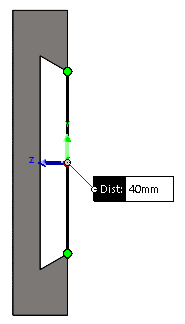
\includegraphics[width=4cm]{figures/fecske_belso}
\caption{A fecskefarok horony minimum távolsága}
\label{Fig:fecske_belso}
\end{figure}
\begin{equation}
\dfrac{\sigma_y}{n}=\dfrac{F}{A}\ \ \ \Rightarrow\ \ \ A=\dfrac{N}{\dfrac{\sigma}{n}}\ \ \ \Rightarrow\ \ \ h\cdot w=\dfrac{N}{\dfrac{\sigma}{n}}\ \ \ \Rightarrow\ \ \ h=\dfrac{N}{\dfrac{\sigma}{n}\cdot w}
\end{equation}
\begin{equation*}\label{Eq:fecske_belso}
h=\dfrac{100000\ [N]}{\dfrac{300\ [MPa]}{4}\cdot 80\ [mm]}=16,67\ [mm]
\end{equation*}

A kiszámolt érték alapján a tervezett alkatrész mérete megfelelőnek bizonyul, mivel a számolt minimum érték kisebb, mint a tervezett méret.

A keménypofa anyaga 1.2312 jelzésű acél, és a horonynak az alján lévő élek és a pofa szélei közötti távolságot kell figyelembe venni. A méretezés során az alábbi képletet használtam:

\begin{figure}[H]
\centering
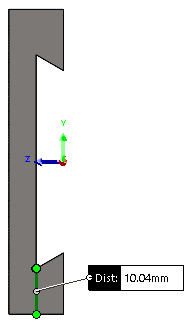
\includegraphics[width=4cm]{figures/fecske_kulso}
\caption{A fecskefarok horony és a pofa széle közötti távolság}
\label{Fig:fecske_kulso}
\end{figure}
\begin{equation}
\dfrac{\sigma_y}{n}=\dfrac{F}{A}\ \ \ \Rightarrow\ \ \ A=\dfrac{N}{\dfrac{\sigma}{n}}\ \ \ \Rightarrow\ \ \ h\cdot w=\dfrac{N}{\dfrac{\sigma}{n}}\ \ \ \Rightarrow\ \ \ h=\dfrac{N}{\dfrac{\sigma}{n}\cdot w}
\end{equation}
\begin{equation*}\label{Eq:fecske_kulso}
h=\dfrac{100000\ [N]}{\dfrac{820\ [MPa]}{4}\cdot 80\ [mm]}=6,1\ [mm]
\end{equation*}

Itt is a kiszámolt érték alapján megállapítható, hogy a tervezett alkatrész mérete megfelelő, mert a számolt minimum érték kisebb, mint a tervezett méret.

\textbf{Összegzés:} A méretezési folyamat tehát két lépésből állt, ahol az egyik alkatrész anyaga C45, míg a másiké 1.2312 jelzésű acél volt. Mindkét esetben a kiszámolt méretek alapján a tervezett alkatrészek mérete megfelelőnek ítélhető. A biztonsági tényező (n=4) alkalmazásával biztosítottam, hogy az alkatrészek a tervezett terhelések alatt is stabilak és biztonságosak lesznek.

Ez a méretezési folyamat igen fontos, hiszen az anyag tulajdonságai (folyáshatár), a terhelési viszonyok és a biztonsági tényezők együttesen határozzák meg, hogy az alkatrészek képesek lesznek-e ellenállni a működés során rájuk nehezedő terheléseknek.
\newpage

\section{Modellezés}
\subsection{Betét}
Első lépésként létrehoztam a betét befoglaló testét, ami egy 25,9 x 57 x 10 milliméteres téglatest volt. Ezt követően létrehoztam a rovátkoláshoz szükséges kivágást, majd a felületen 0,57 mm-es osztással kiosztottam, hogy megkapjam a végleges rovátkolt felületet.
\begin{figure}[H]
\centering
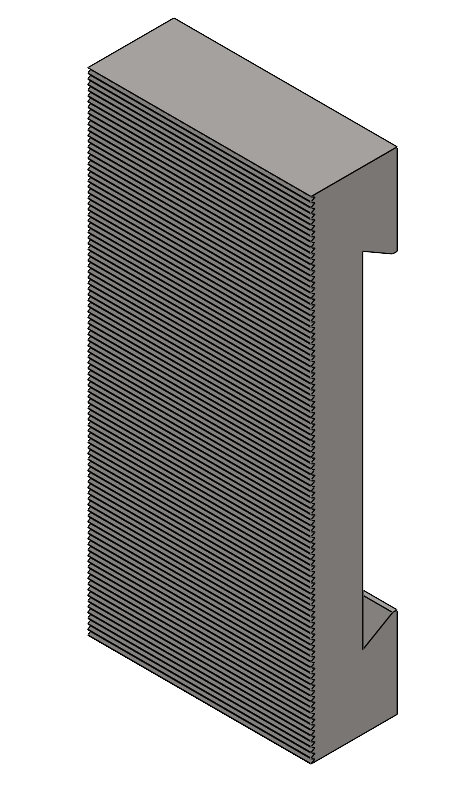
\includegraphics[width=6cm]{figures/betet_rovatkolas}
\caption{A betét kialakítása a rovátkolással}
\label{Fig:betet_rovatkolas}
\end{figure}

A betét próbatest felőli részére nem kell több alakelem, tehát áttérhettem a betét alaptest felőli oldalára. Ezen az oldalon létre kellett hozni a \glqq fecskefarok\grqq\ vezetéket, valamint a pozícionáló furatot. A vezetékhez elsőként megrajzoltam a szükséges vázlatot, aminek a méretét a szerszámkatalógusban található szögmaró adataiból megállapítottam, majd ezt a vázlatot kivágtam a modellből. Végül a pozícionáló furatot készítettem el szintén kivágással.

\begin{figure}[H]
\centering
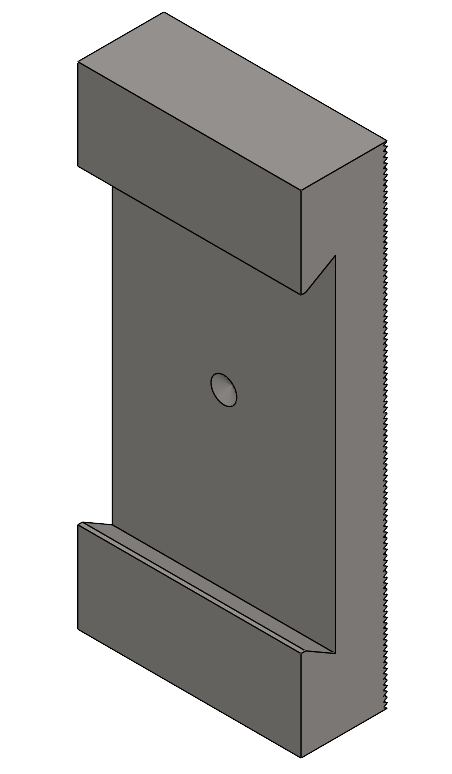
\includegraphics[width=4.5cm]{figures/betet_pozicio}
\caption{A betét \glqq fecskefarok\grqq\ vezeték része és a pozíciót biztosító jelölés}
\label{Fig:betet_pozicio}
\end{figure}

Miután elkészítettem az egyik oldali betétet, létre kellett hoznom a betét ellendarabját. Ehhez a betéthez a feljebb leírt módon elkészítettem a modellt, azonban a rovátkolást fél osztással eltoltam, hogy illeszkedjen a két fél, és ne  hozzon létre vágó hatást a próbatesten.

\subsection{Alaptest}
Az alaptest modelljének létrehozásához szükséges megállapítani a gyári szakítópofa ékszögét, mellyel csatlakozik a szakítógéphez. Egy precíziós szögmérőt alkalmaztam, azzal megállapítottam hogy az ékszög 75° volt. Ezt követően létrehoztam a befoglaló testet, aminek 57 x 23,5 x 25,9 mm mérete van.

\begin{figure}[H]
\centering
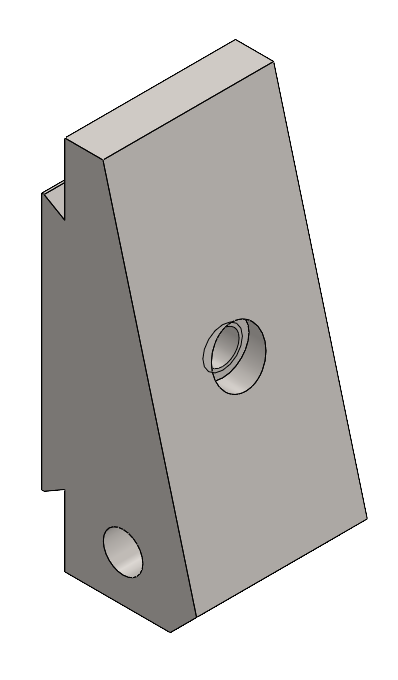
\includegraphics[width=4.5cm]{figures/alaptest_ek}
\caption{Az alaptest ék része}
\label{Fig:alaptest_ek}
\end{figure}

Ezután létrehoztam az éket egy kivágással, majd ezután a \glqq fecskefarok\grqq\ vezeték belső részét szintén egy kivágással. Szükséges létrehozni egy furatot a modell oldalában, mert abba illeszkedik majd egy egyedileg módosított illesztőszeg, amely azt a célt szolgálja, hogy amikor a szakítópofát kilazítjuk, az illesztőszegre helyezett rugó szétnyitja a pofákat, hogy ki tudjuk venni a próbatestet.

Az alaptestben kell létrehozni egy furatot, amibe a golyót, a rugót és a hernyócsavart tesszük, ami biztosítja a betét pozícióját.

\begin{figure}[H]
\centering
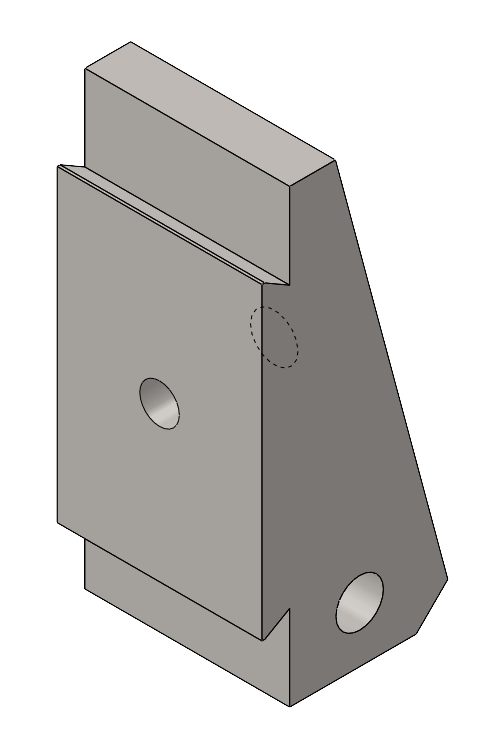
\includegraphics[width=6cm]{figures/alaptest_vezetek}
\caption{Az alaptest \glqq fecskefarok\grqq\ vezeték része}
\label{Fig:alaptest_vezetek}
\end{figure}

\begin{figure}[H]
\centering
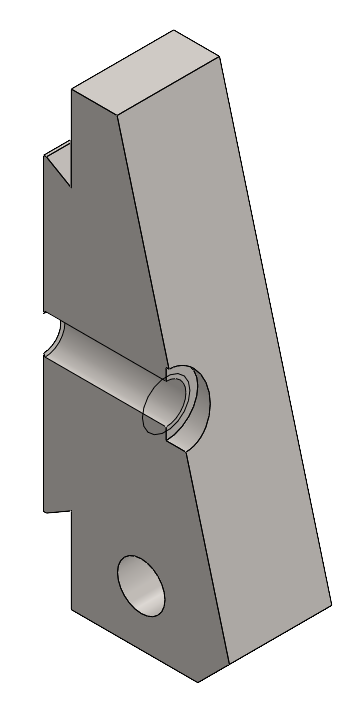
\includegraphics[width=4cm]{figures/alaptest_furat}
\caption{Az alaptest furata a betét pozícióját biztostó alkatrészeknek}
\label{Fig:alaptest_furat}
\end{figure}

\subsection{Összeállítás}
Az alkatrészek modellezését követően jön a szerkezet összeállítása. Ebben a fázisban a saját tervezésű alkatrészek mellett kereskedelemben kapható elemek és kötőelemek is felhasználásra kerülnek. Az összeállítás során a valósághű szerelési kényszereket figyelembe véve építem fel a szerkezetet, amit az alábbi ábrán szemléltettem. Ez magában foglalja a különböző alkatrészek helyes illesztését, a kötőelemek megfelelő alkalmazását, és az összeszerelés során fellépő dinamikai és statikai interakciók figyelembevételét.
\begin{figure}[H]
    \centering
    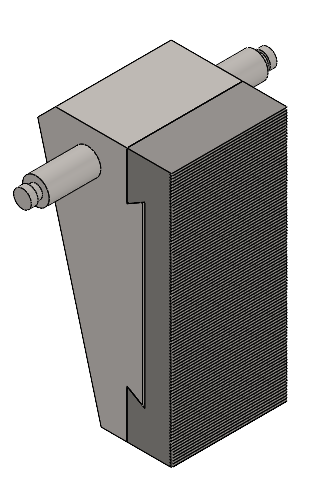
\includegraphics[width=4.5cm]{figures/Assembly_1.png}
    \caption{Összeszerelt szakítópofa egység}
    \label{Fig:Assembly_1}
\end{figure}

A pozíciót biztosító megoldás részletei az alábbi \ref{Fig:Assembly_2}. ábrán tekinthetők meg. Ez a megoldás a szerkezet pontos és stabil helyzetét garantálja a szakítóvizsgálat elvégzése során.
\begin{figure}[H]
    \centering
    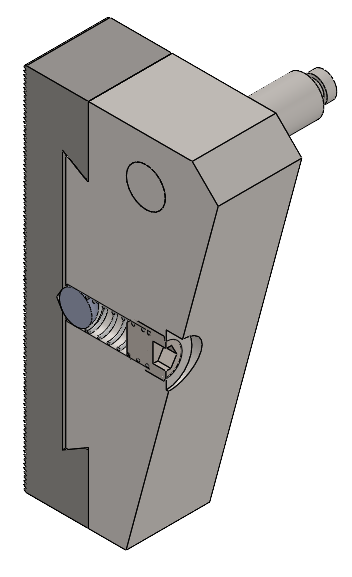
\includegraphics[width=4.5cm]{figures/Assembly_2.png}
    \caption{Összeszerelt egység metszeti ábrázolása}
    \label{Fig:Assembly_2}
\end{figure}

A külön-külön összeszerelt egységeket egy nagyobb, komplexebb összeállításba integráltam, ezzel létrehozva a teljes szakító egységet. Ennek érdekében egy \glqq kutyacsont\grqq\ alakú próbatestet modelleztem, amely szemléletesen mutatja be, hogyan fog kinézni és működni az összeállítás a gyakorlatban. Ez a próbatest lehetővé teszi a teljes rendszer tesztelését, valós körülmények közötti viselkedésének megfigyelését és a szükséges finomhangolások elvégzését. A fő összeállítás, amely tartalmazza az egyedi és kereskedelmi alkatrészeket, valamint a kutyacsont alakú próbatestet, az alábbi \ref{Fig:Assembly_3}. ábrán látható. Ez az ábra részletes betekintést nyújt a szakító egység teljes szerkezetébe és az egyes komponensek egymáshoz viszonyított elhelyezkedésébe.
\begin{figure}[H]
    \centering
    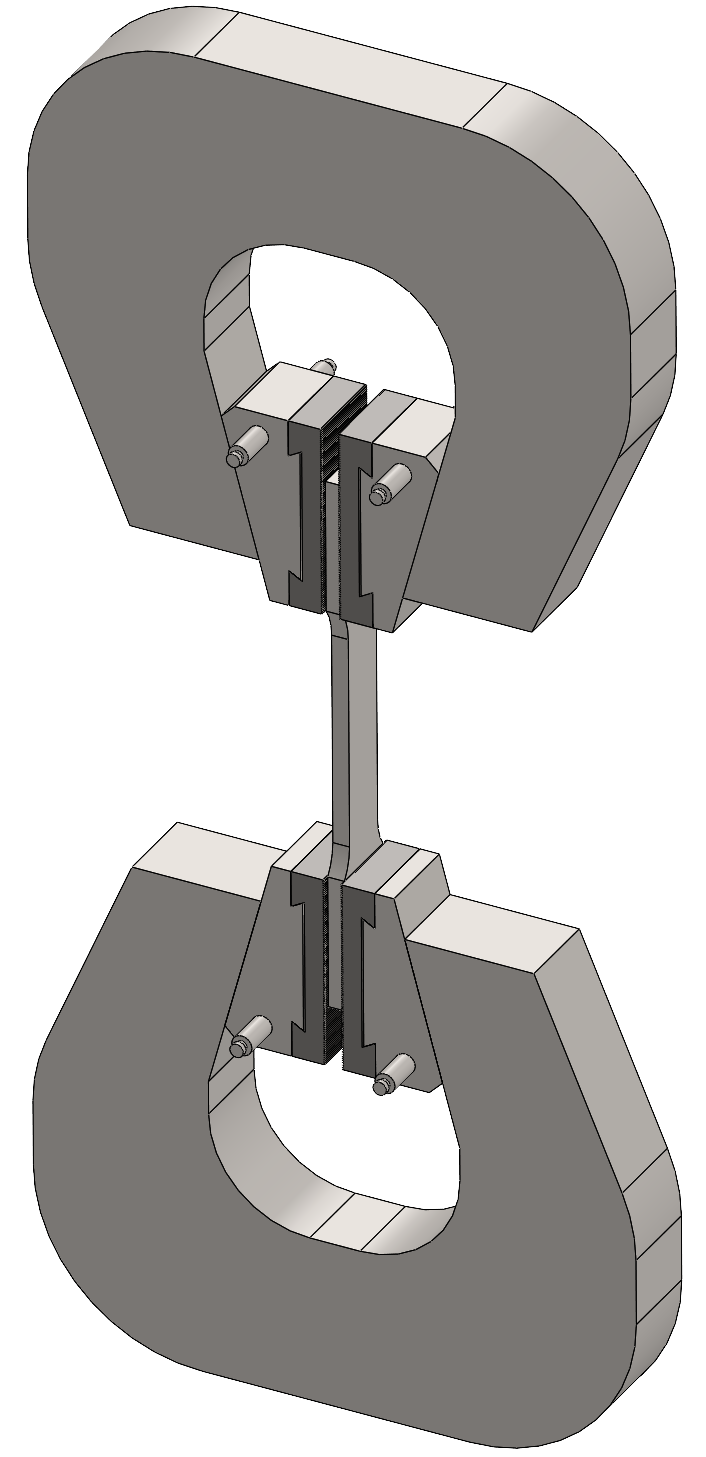
\includegraphics[width=11cm]{figures/Assembly_3.png}
    \caption{A fő összeállítás}
    \label{Fig:Assembly_3}
\end{figure}

\chapter{Végeselem analízis}
%\todo[inline]{ezt a részt még kicsit ki kell egészíteni}
\section{Előkészítés}
A létrehozott főösszeállítást elsőként a CAD szoftverből ki kell exportálni a megfelelő kiterjesztésben. Ez lehet például .step vagy .iges. Miután ez elkészült, el kell indítani a végeselem analízis szoftvert, ami jelen esetben az Ansys Workbench 2023 R2 szimulációs környezet.
A főképernyőn lehetőségünk van kiválasztani a számunkra megfelelő szimulációs modult (pl. Static Structural, Modal, Explicit Dynamics). A szakdolgozat során elég a \glqq Static Structural\grqq\ modul, ez az egyszerű statikus vizsgálat, amelynél nem számít az idő változása.
\begin{figure}[H]
    \centering
    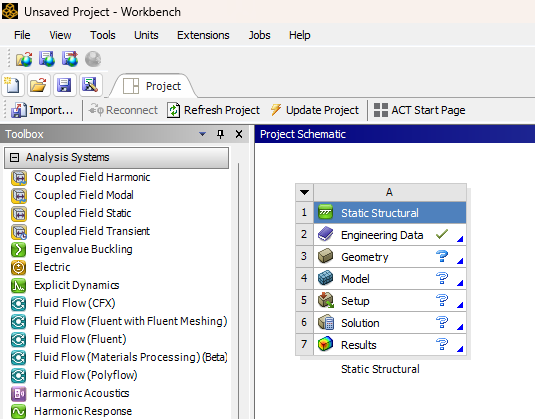
\includegraphics[width=12cm]{figures/ansys_1.png}
    \caption{Ansys Workbench főképernyő}
    \label{Fig:ansys_1}
\end{figure}

\subsection{Anyagmodellek létrehozása}
Miután kiválasztottam a \glqq Static Structural\grqq\ modult, lehetőségem van beállítani a szükséges anyagmodelleket. A szimuláció során lineáris anyagmodellt alkalmazok minden alkatrészre. A beállításhoz elegendő megadni a rugalmassági (Young) moduluszt és a Poisson tényezőt, azonban én beállítottam a sűrűséget, a folyáshatárt és a szakítószilárdságot is.

\begin{figure}[H]
    \centering
    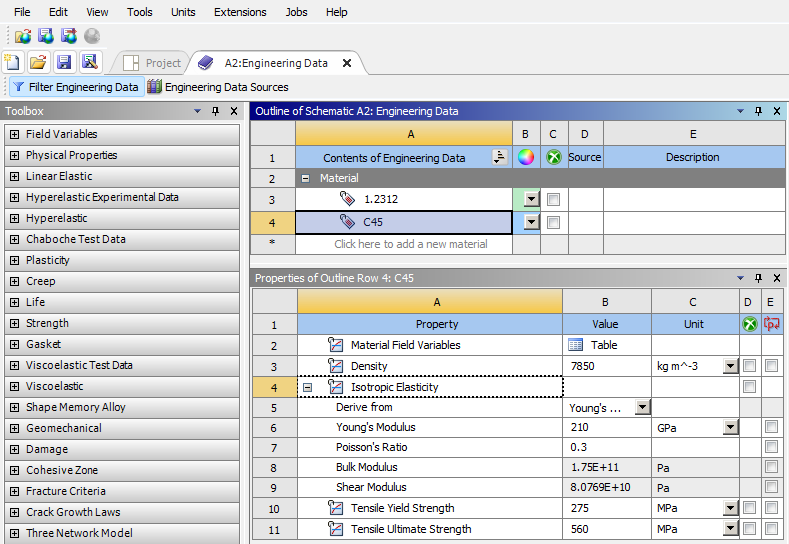
\includegraphics[width=15cm]{figures/ansys_2.png}
    \caption{Beállított anyagmodellek}
    \label{Fig:ansys_2}
\end{figure}

Az anyagmodellek beállítására kiemelt figylemet kell fordítani, mert a szimuláció lefutását, valamint a szimuláció eredményét nagymértékben befolyásolhatja. A szakítófejet rugalmas test helyett szilárd testre állítottam, mivel a valósághoz hasonlóan a vizsgálat szempontjából is elhanyagolható mértékben deformálódik, illetve a feszültségértékek is elhanyagolhatóan minimálisak. A próbatest anyagának a vizsgálat elvégzéséhez szerkezeti acélt választottam.

\subsection{Diszkretizálás}
A 3D modell diszkretizálása során a testet felbontjuk kisebb elemekre. A diszkretizálással minden elemnek önálló merevségi mátrixa lesz, melyeket a szoftver összeilleszt és az egész testre vonatkozó merevségi mátrix-szal számol. Ez a folyamat, amíg a szoftver elvégzi a szükséges számításokat, a háló finomságának a függvényében a pár másodperctől egészen a több órás időtartamig változhat.

Az modellen kvadratikus hálót állítottam be, mivel tartalmaz íves elemeket. Ezzel a módszerrel kevesebb elemre van szükség a test felbontásához, de a magasabb függvényfoka miatt bonyolultabb számításokat igényel. Az egész testre vonatkozó elemméretet 10 mm-re állítottam be. A teljes testnek a hálózását az alábbi \ref{Fig:mesh_2}. ábrán lehet látni.

\begin{figure}[H]
    \centering
    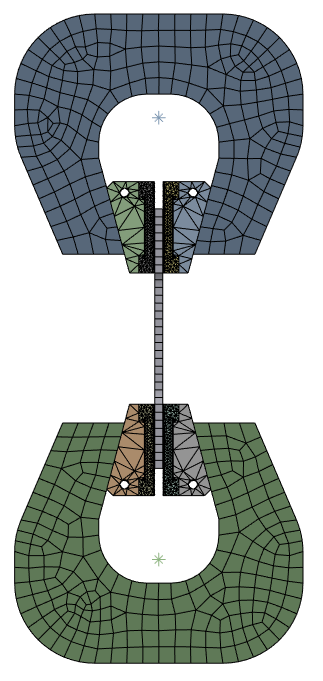
\includegraphics[width=7cm]{figures/mesh_2.png}
    \caption{A szerkezet kész hálózása}
    \label{Fig:mesh_2}
\end{figure}

\subsubsection{Háló finomítás}
Az alap elemmérettel a szimuláció elvégzése nem lehetséges, mert a keménypofa rovátkolása sokkal kisebb méretű, mint 10 mm. A durva háló a geometriai tulajdonságok elvesztéséhez, valamint a szimuláció eredményeinek pontatlanságához vezethet. Ezért szükséges háló finomítást alkalmazni az érintett alkatrészeken. Jelen esetben a keménypofán, valamint a szakító próbatesten érdemes sűríteni a hálót. A keménypofán 2 mm-es, míg a próbatesten 5 mm-es elemméretet alkalmaztam. Ez hosszabb futási időt eredményez, de megtartja a keménypofa geometriáját, valamint pontosabb eredmények várhatóak a szimuláció elvégeztével. Az alábbi ábrán a sűrített háló látható.

\begin{figure}[H]
    \centering
    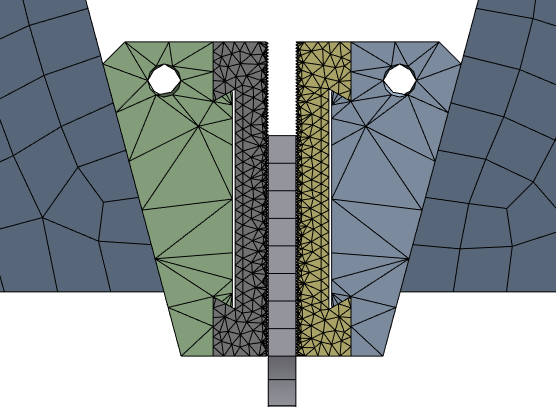
\includegraphics[width=9cm]{figures/mesh_3.png}
    \caption{A sűrített háló a keménypofán és a próbatesten}
    \label{Fig:mesh_3}
\end{figure}

\subsection{Kényszerek, terhelések}
A szimuláció megkezdése előtt fontos definiálni a modellen a szükséges kényszereket, amelyek a modell szabadságfokait kötik le a valós viszonyoknak megfelelően. Szükséges volt a szerkezet síkbeli megkötése, hogy csak a húzási irányba tudjon elmozdulni. Az alsó szakítófejnek az alsó síkját egy fix kényszerrel lekötöttem, hogy ne tudjon elmozdulni. Az alkatrészek surlódásos kontakttal állnak kapcsolatban egymással, ami azt jelenti hogy a valóságnak megfelelően tudtam elhelyezni a terheléseket a modellen.

A kényszerek definiálása után a terheléseket kellett elhelyezni a szerkezeten. Elsőként a valós körülményekhez igazodva megadtam a szakítópofák kézi meghúzásának megfelelő 500 N-os előterhelést, majd ezt követően a vizsgálathoz a felső szakítófejen alkalmaztam egy 2 mm-es elmozdulást, ami elegendő a kívánt eredmény eléréséhez. A surlódásos kapcsolat miatt a szerkezet valós működésével azonosan, itt is nő a szakítópofák szorítóereje a vizsgálat sorás a szakítópofa ékhatásának köszönhetően.

\subsection{Szimuláció beállításai}
A szimuláció végrehajtásához elsőként beállítottam a \glqq Large Deflection\grqq-t , ami a nagy elmozdulások miatt minden iteráció alkalmával újraszámolja a merevségi mátrixot, ezáltal nagy elmozdulások esetén pontosabb eredmény lehet elérni vele. Továbbá szükséges volt a szimulációt idejét \glqq Substep\grqq-ekre osztani, mivel a kisebb lépések pontosabb számítást tesznek lehetővé.

\section{Eredmények kiértékelése}
A szimuláció sikeres lefutását követően az eredmények kiértékelése volt a következő feladat. A szimulóció eredményeként az elmozdulást, valamint a von-Mises-féle ekvivalens feszültségértéket értékeltem ki.

\subsection{Elmozdulás}
Az alábbi \ref{Fig:mesh_5}. ábrán látható, hogy a szakítóvizsgálat vizsgálati hossza 2 mm volt. Ez az érték a próbatest vizsgálatához elegendő, elég nagy feszültségértékek várhatóak ahhoz, hogy a próbatest eltörjön.

\begin{figure}[H]
    \centering
    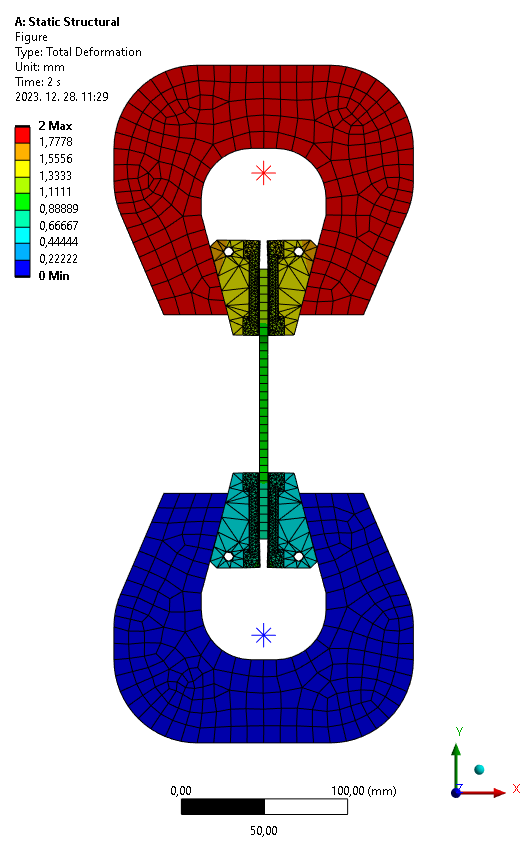
\includegraphics[width=10cm]{figures/mesh_5.png}
    \caption{Teljes elmozdulás}
    \label{Fig:mesh_5}
\end{figure}

\subsection{Feszültség}
A másik, a tervezés szempontjából fontosabb kiértékelés a von-Mises-féle ekvivalens feszültség volt. Itt fontos megjegyezni, hogy a vizsgálathoz használt anyagmodellek lineáris tulajdonságúak, ezért a vizsgálat is a lineáris szakaszon történt. Ahogy az alábbi ábrán látható, a szerkezetben ébredő maximális feszültséget nem kell figyelembe venni, mert a próbatest feltételezhető törési helyén, vagyis a vizsgálati hossz közepén 491,5 MPa feszültség mérhető, ami meghaladja a szerkezeti acélok folyáshatárát.

\begin{figure}[H]
    \centering
    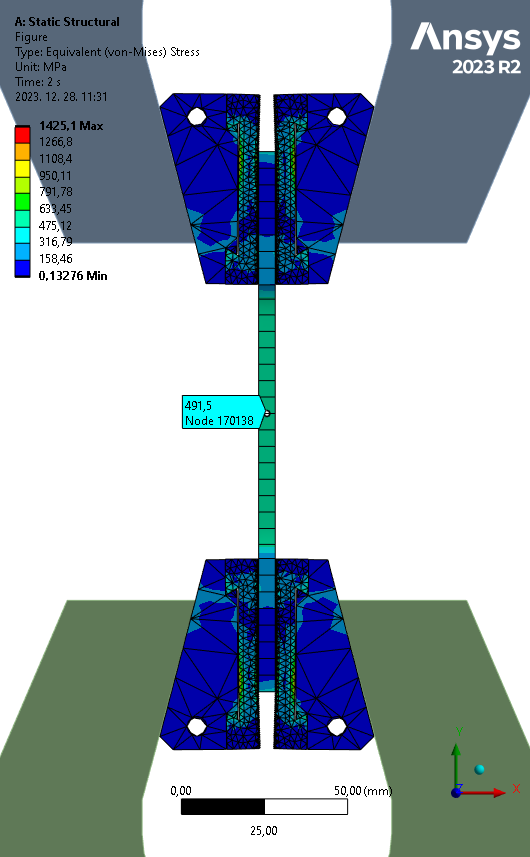
\includegraphics[width=10cm]{figures/mesh_6.png}
    \caption{Teljes elmozdulás}
    \label{Fig:mesh_6}
\end{figure}

A végeselem szimuláció kiértékelését követőne meg tudtam állapítani, hogy a geometria megfelelő lesz, ezért elkezdhettem megtervezni az alkatrészek gyártását CAM programban.

\chapter{Gyártás}
\section{Előkészítés}
Az alkatrészek gyártásának előkészítésének legelső lépése az alkatrészek műszaki rajzának az elkészítése. Az alaptest és a keménypofa műszaki rajzai a mellékletek között találhatók.
\subsection{Előgyártmány}
Az alkatrészek előgyártmányát ergonomic 320.250 G típusú szalagfűrésszel daraboltam le. A keménypofának egy 30x20 mm-es keresztmetszetű, az alaptestnek pedig egy 32x30 mm-es keresztmetszetű laposacélt fűrészeltem 65 mm hosszúra.

\section{CAM}
%\todo[inline]{CNC típusa}
A gyártás előkészítése után el kell készíteni az alkatrészek CAM programját. Ezt én a Solidworks bővítményeként elérhető Autodesk HSMWorks CAM szoftverrel készítettem el. A gyártáshoz a Gyártástechnológia laborban található Akira Seiki 3 tengelyes megmunkálóközpontot használtam. A gyártáshoz használt szerszámok az alábbiakban lesznek részletezve, a megmunkálási műveleteknél.
\subsection{Keménypofa}
Elsőként a keménypofának a programját készítettem el. Az alábbi szekciókban a műveleteket listázom, ahol részletesebben kifejtem a forgácsolási paramétereket.

\subsubsection{Síkmarás - 1.}
A síkmarást a Gyártástechnológia laborban megtalálható Sandvik márkájú síkmaróval végeztem.

\textbf{Adatok, paraméterek}
\begin{itemize}
    \item Alaptest: 345-063Q22-13M
    \item Lapka: 345R-1305E-PL 4330
    \item Vágósebesség ($v_c$): 367 m/min
    \item Fogankénti előtolás ($f_z$): 0,141 mm
    \item Élek száma ($z$): 5 db
\end{itemize}
\begin{figure}[H]
    \centering
    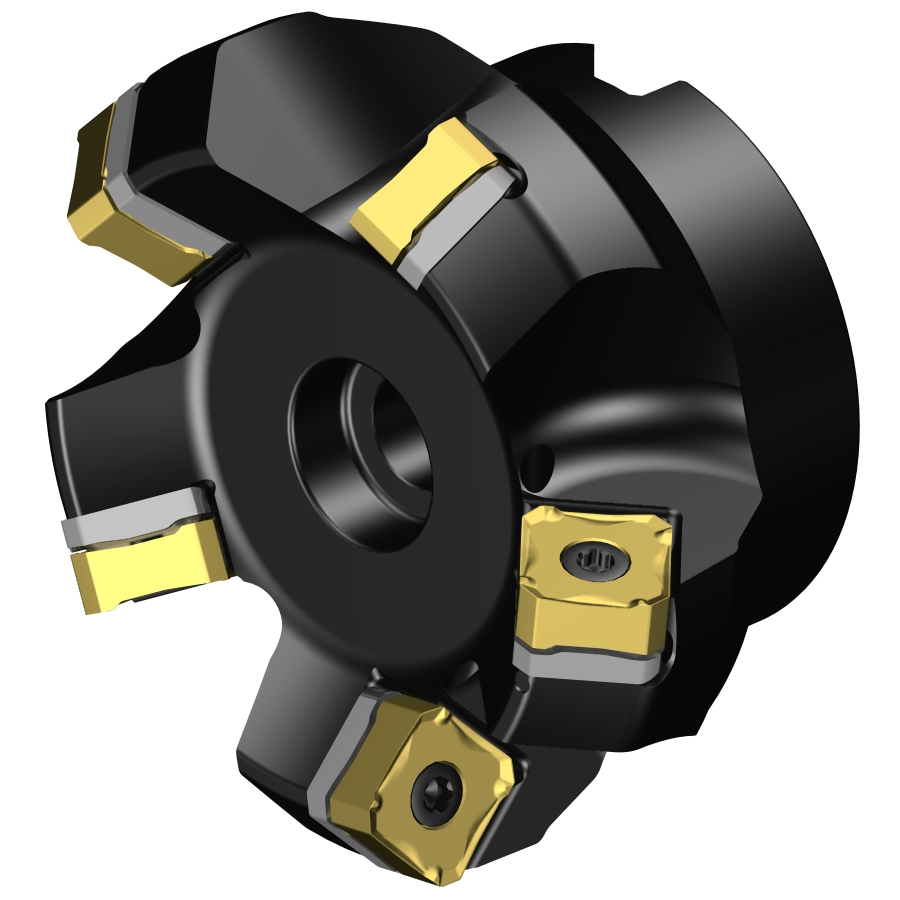
\includegraphics[width=5cm]{figures/facemill.jpg}
    \caption{Sandvik síkmaró}
    \label{Fig:facemill}
\end{figure}
Kiszámítottam a vágósebességhez tartozó fordulatszámot ($n$), illetve az előtolási sebességet ($v_f$) az alábbi \ref{Eq:facemill_vc}. és \ref{Eq:facemill_vf}. egyenletekkel.
\begin{equation}\label{Eq:facemill_vc}
    n=\dfrac{v_c\cdot1000}{D\cdot\pi}=\dfrac{367\cdot1000}{63\cdot\pi}=1854\ \dfrac{1}{min}
\end{equation}
\begin{equation}\label{Eq:facemill_vf}
    v_f=f_z\cdot z\cdot n=0,141\cdot5\cdot1854=1307\ \dfrac{mm}{min}
\end{equation}

A szerszám beállítása után beállítottam a síkmarás paramétereit, a fogásmélységet, a rá- és leállást. Az \ref{Fig:kemenypofa_facemill_1}. ábrán a síkmarás elkészült szerszámpályája látható.

\begin{figure}[H]
    \centering
    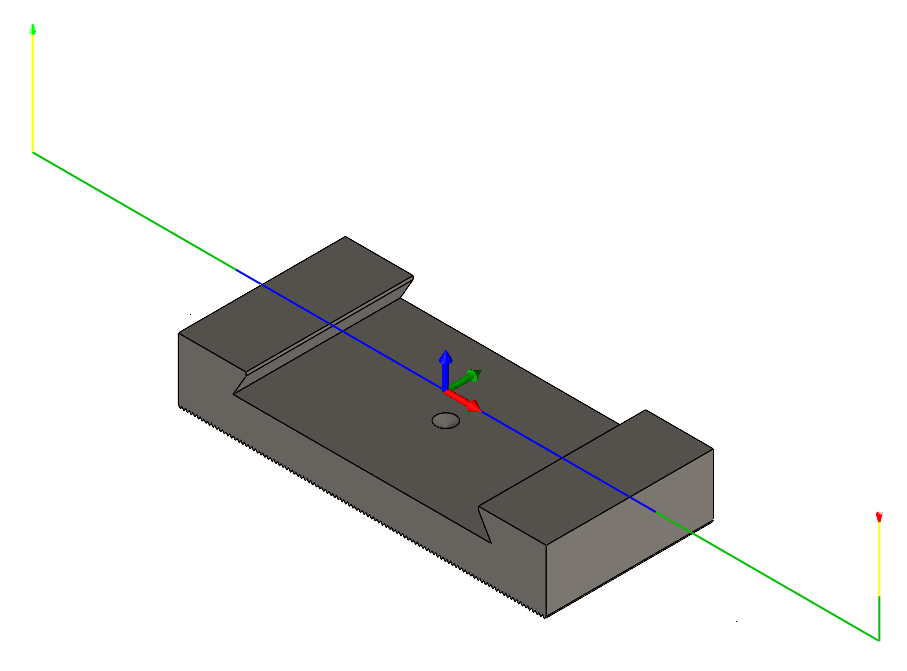
\includegraphics[width=12cm]{figures/kemenypofa_facemill_1.png}
    \caption{Az első síkmarás szerszámpályája}
    \label{Fig:kemenypofa_facemill_1}
\end{figure}


\subsubsection{Kontúrmarás}
A síkmarás után a keménypofának a külső kontúrját kellett nagyolni. A nagyoláshoz és a simításhoz is ugyanolyan típusú Kennametal szármarót alkalmaztam. A marót egy patronos, hidraulikus, vagy zsugorkötéses alaptestbe kell tenni, jelen esetben a laborban megtalálható patronos alaptestet választottam. Szükséges volt megállapítani a maximális fogásmélységet, ez határozza meg a maró forgácsolási élhosszát és a CAM programban ez szerint kell beállítani a maró geometriáját, az ütközésvizsgálat helyes működéséhez.

\begin{figure}[H]
    \centering
    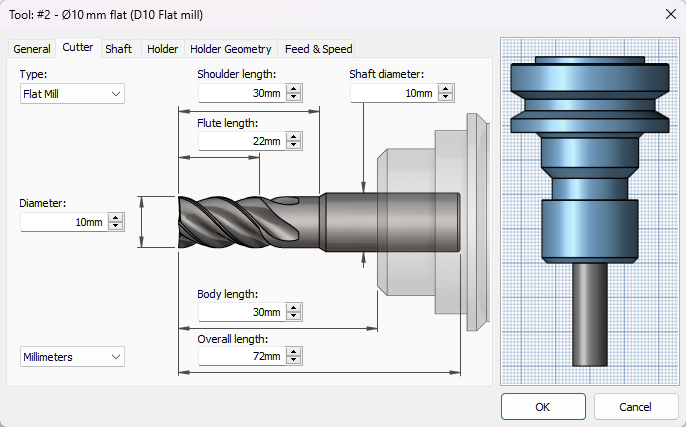
\includegraphics[width=12.5cm]{figures/d10_flat_geometry.png}
    \caption{Kennametal D10 szármaró geometriája a CAM rendszerben}
    \label{Fig:d10_flat_geometry}
\end{figure}

\textbf{Adatok, paraméterek}
\begin{itemize}
    \item Maró: H1TE4SE1000N022HAM - KCPM15
    \item Vágósebesség ($v_c$): 165 m/min
    \item Fogankénti előtolás ($f_z$): 0,13 mm
    \item Élek száma ($z$): 4 db
    \item Axiális irányú fogás ($a_p$): 10,5 mm
    \item Oldalirányú fogás ($a_e$): 0,5 mm
\end{itemize}

\begin{figure}[H]
    \centering
    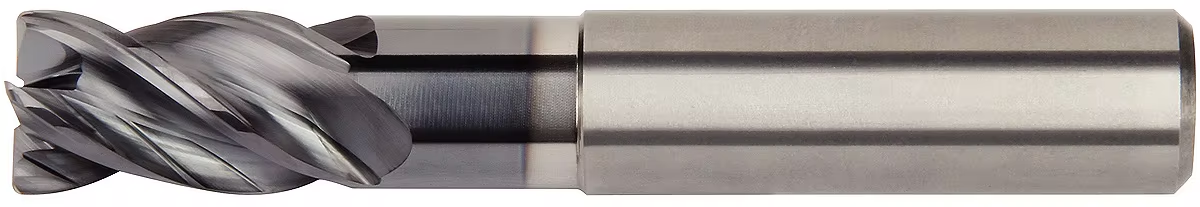
\includegraphics[width=6cm]{figures/d10_flatmill.png}
    \caption{Kennametal D10 szármaró}
    \label{Fig:d10_flatmill}
\end{figure}

Az alábbiakban kiszámítottam az \ref{Eq:facemill_vc}. és \ref{Eq:facemill_vf}. egyenletekkel a szármaróhoz tartozó fordulatszámot és az előtolási sebességet.

\begin{equation*}
    n=\dfrac{v_c\cdot1000}{D\cdot\pi}=\dfrac{165\cdot1000}{10\cdot\pi}=5252\ \dfrac{1}{min}
\end{equation*}
\begin{equation*}
    v_f=f_z\cdot z\cdot n=0,13\cdot4\cdot5252=2731\ \dfrac{mm}{min}
\end{equation*}

A szerszám geometriája, valamint a forgácsolási paraméterek beállítása után meg kellett határozni a nagyolási stratégiát. Én az állandó forgácskeresztmetszetet biztosító \glqq2D Adaptive\grqq\ megmunkálást választottam, mivel ez a legalkalmasabb az ehhez hasonló alkatrészek kontúrjának nagyolásához.

\begin{figure}[H]
    \centering
    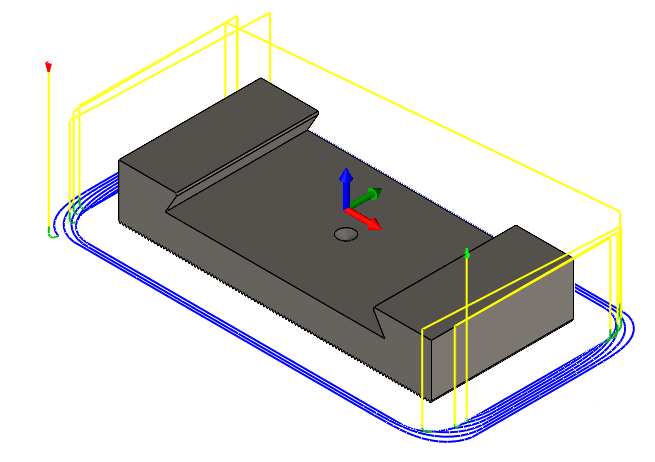
\includegraphics[width=10cm]{figures/kemenypofa_adaptive_1.png}
    \caption{Keménypofa 2D Adaptive kontúr nagyolása}
    \label{Fig:kemenypofa_adaptive_1}
\end{figure}

A kontúr felületen hagytam 0,5 mm simítási ráhagyást, melyet egy egyszerű kontúrmarással távolítottam el. A CAM programban beállítottam, hogy a CNC vezérlőben tárolt szerszámkorrekció szerint végezze a kontúr simítását, mert idővel a szerszámok kopnak, ezért folyamatosan változhat a szerszám sugara. A forgácsolási paraméterek maradhatnak, mert ezt a műveletet is egy, az előzővel egyező maróval végeztem el.

\begin{figure}[H]
    \centering
    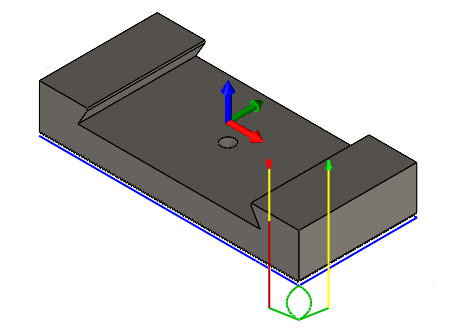
\includegraphics[width=12cm]{figures/kemenypofa_contour_1.png}
    \caption{Keménypofa külső kontúrjának simítása}
    \label{Fig:kemenypofa_contour_1}
\end{figure}

\subsubsection{Fecskefarok horony nagyolás}
A külső kontúr nagyolása és simítása után a következő lépés a fecskefarok horony nagyolása volt. A horony nagyolását az előző kontúr nagyolási műveletnél használt D10 szármaróval végeztem el.

Ennél a műveletnél az axiális irányú fogásvétel kisebb lesz, ezért az oldalirányú fogásvétel növelésével törekedtem az előző nagyolási művelethez hasonló forgácskeresztmetszet elérésére.

A fecskefarok horony nagyolásának forgácsolási paraméterei az axiális és oldalirányú fogásvétel kivételével változatlanok. A fecskefarok horony simítási ráhagyását itt is 0,5 mm-re állítottam. A simítást a korábbihoz hasonlóan egy, a nagyoláshoz használt maróval egyező szerszámmal végeztem el.

\textbf{Adatok, paraméterek}
\begin{itemize}
    \item Axiális fogásvétel ($a_p$): 4 mm
    \item Oldalirányú fogásvétel ($a_e$): 1 mm
\end{itemize}

\begin{figure}[H]
    \centering
    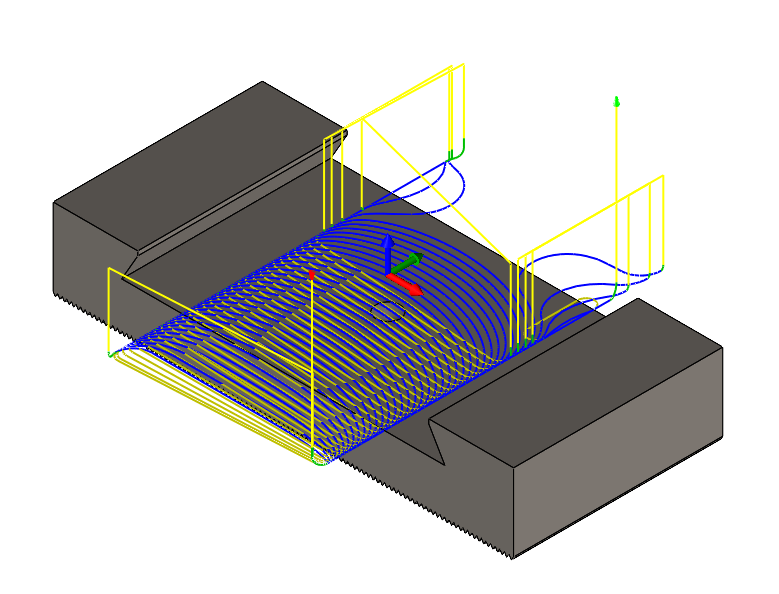
\includegraphics[width=12cm]{figures/kemenypofa_dovetail_1.png}
    \caption{Fecskefarok horony nagyolása}
    \label{Fig:kemenypofa_dovetail_1}
\end{figure}

\begin{figure}[H]
    \centering
    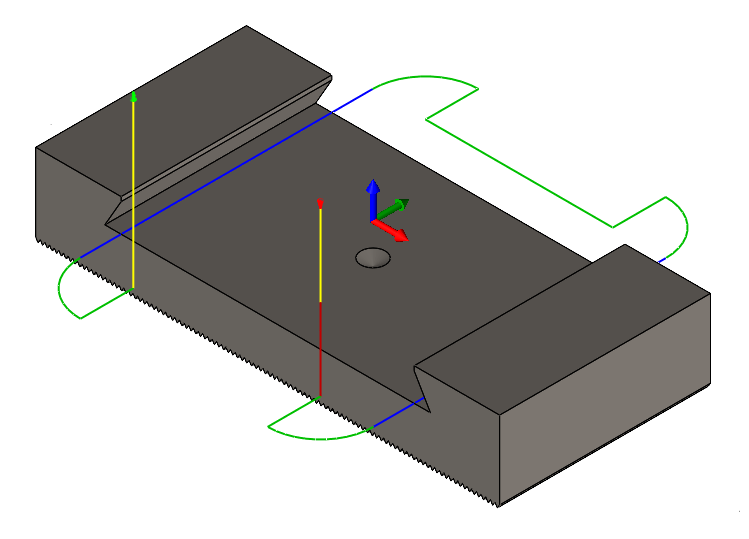
\includegraphics[width=11.5cm]{figures/kemenypofa_dovetail_2.png}
    \caption{Fecskefarok horony oldalának simítása}
    \label{Fig:kemenypofa_dovetail_2}
\end{figure}

\subsubsection{Fecskefarok horony}
%\todo[inline]{Szerszám forgácsolási paraméterek}
A fecskefarok horony kialakításához egy 60°-os szögmarót kellett keresnem. A Hoffmann Group katalógusában sikerült találnom Garant márkájú, bevonat nélküli HSS szögmarót, amely alkalmas lesz a megmunkálásra.

\begin{figure}[H]
    \centering
    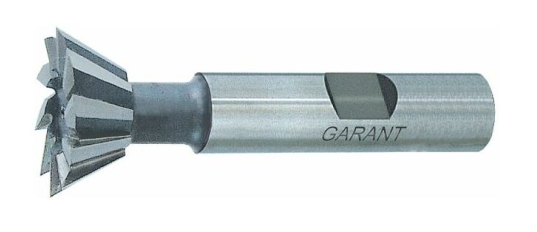
\includegraphics[width=10cm]{figures/szogmaro.png}
    \caption{Garant HSS szögmaró}
    \label{Fig:szogmaro}
\end{figure}

Ahogy a már a korábbi szerszámoknál, itt is először be kellett állítanom a szerszám geometriáját, majd ezután a forgácsolási paramétereket.

\textbf{Adatok, paraméterek}
%\todo[inline]{szerszám forgácsolási paraméterek}
\begin{itemize}
    \item Megnevezés: Száras szögmaró, Form C 60° bevonat nélkül
    \item Vágósebesség ($v_c$): 25 m/min
    \item Fogankénti előtolás ($f_z$): 0,05 mm
    \item Oldalirányú fogásvétel ($a_e$): 0,5 mm
    \item Fogások száma: 6
    \item Simító fogás: 0,1 mm
\end{itemize}

\begin{figure}[H]
    \centering
    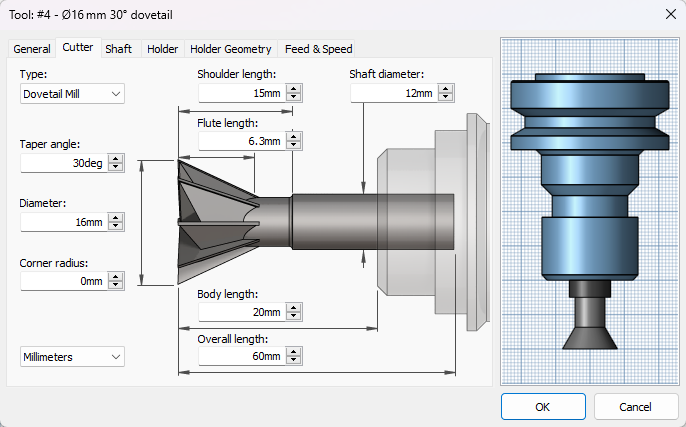
\includegraphics[width=12cm]{figures/dovetail_geometry.png}
    \caption{Szögmaró geometriája a CAM programban}
    \label{Fig:dovetail_geometry}
\end{figure}

Az alábbiakban meghatároztam a szögmaróhoz tartozó fordulatszámot, valamint az előtolási sebességet az \ref{Eq:facemill_vc}. és \ref{Eq:facemill_vf}. egyenletek szerint.

\begin{equation*}
    n=\dfrac{v_c\cdot1000}{D\cdot\pi}=\dfrac{25\cdot1000}{16\cdot\pi}=497\ \dfrac{1}{min}
\end{equation*}
\begin{equation*}
    v_f=f_z\cdot z\cdot n=0,05\cdot6\cdot497=149\ \dfrac{mm}{min}
\end{equation*}

A CAM programban megadtam a fecskefarok horony kontúrját, beállítottam a fogásvétel nagyságát, valamint megadtam, hogy hány fogásvételt végezzen oldalanként. Miután elvégeztem a szükséges beállításokat, elkészítettem a szerszámpályát.

\begin{figure}[H]
    \centering
    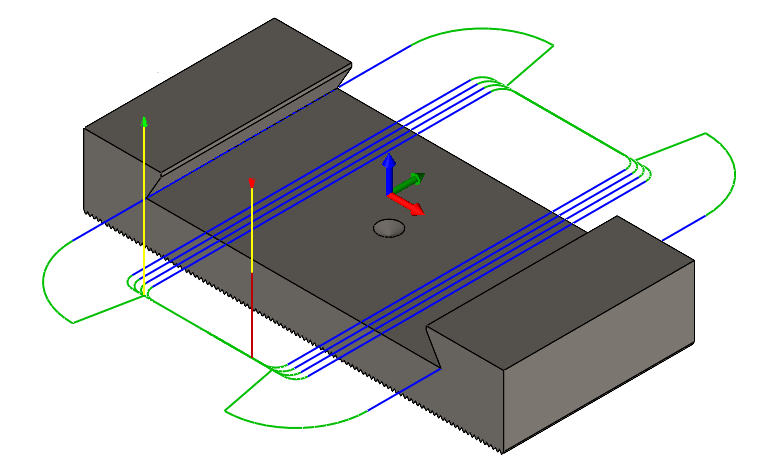
\includegraphics[width=12.5cm]{figures/kemenypofa_dovetail_3.png}
    \caption{Szögmaró szerszámpályája}
    \label{Fig:kemenypofa_dovetail_3}
\end{figure}

\subsubsection{Fúrás}
A keménypofa első befogásának utolsó művelete, a pozíciót biztostó furat elkészítése következett. Ehhez a Kennametal katalógusából egy 5 mm átmérőjű keményfém csigafúrót használtam, mivel az alaptesthez is szükség lesz egy ekkora méretű fúróra az M6-os menet magfuratának elkészítéséhez. A szerszám rögzítésének szintén egy patronos megfogót használtam.

\textbf{Adatok, paraméterek}
\begin{itemize}
    \item Fúró: B225A05000HPX - KCP15B
    \item Vágósebesség ($v_c$): 150 m/min
    \item Előtolás ($f$): 0,15 mm/ford
\end{itemize}

Alább az \ref{Eq:facemill_vc}. egyenlettel kiszámoltam a szükséges fordulatszámot. Az előtolási sebesség megállapításához az \ref{drill_vf}. egyenletet használtam.
\begin{equation*}
    n=\dfrac{v_c\cdot1000}{D\cdot\pi}=\dfrac{150\cdot1000}{5\cdot\pi}=9549\ \dfrac{1}{min}
\end{equation*}

\begin{equation}\label{drill_vf}
    v_f=f\cdot n=0,15\cdot 9549=1432\ \dfrac{mm}{min}
\end{equation}

\begin{figure}[H]
    \centering
    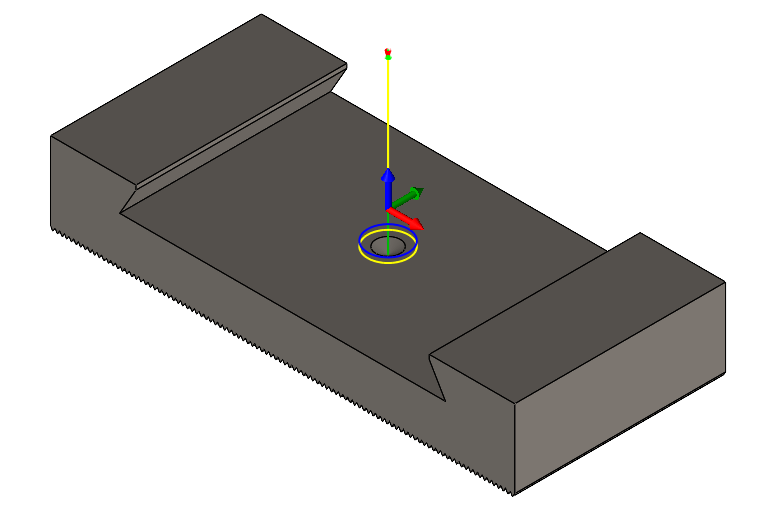
\includegraphics[width=11cm]{figures/kemenypofa_drill.png}
    \caption{Pozícionáló furat CAM programja}
    \label{Fig:kemenypofa_drill}
\end{figure}

A fúrás befejezése után a keménypofának az első megfogása elkészült. A következő alfejezetekben a keménypofa megmunkálásának 2. megfogását tárgyalom. Elsőként definiáltam az új megmunkálási síkokat, valamint a nullpontot.

\subsubsection{Síkmarás - 2.}
A 2. megfogás első művelete az előző megfogásból megmaradt anyag visszamarása. Ezt a korábban használt síkmaróval végeztem el, a forgácsolási paraméterek megegyeznek a korábban használtakkal. A síkmaráshoz 1 mm-es axiális fogásmélységet ($a_p$) adtam meg ezért több fogásból kerül lemunkálásra az anyag.

\begin{figure}[H]
    \centering
    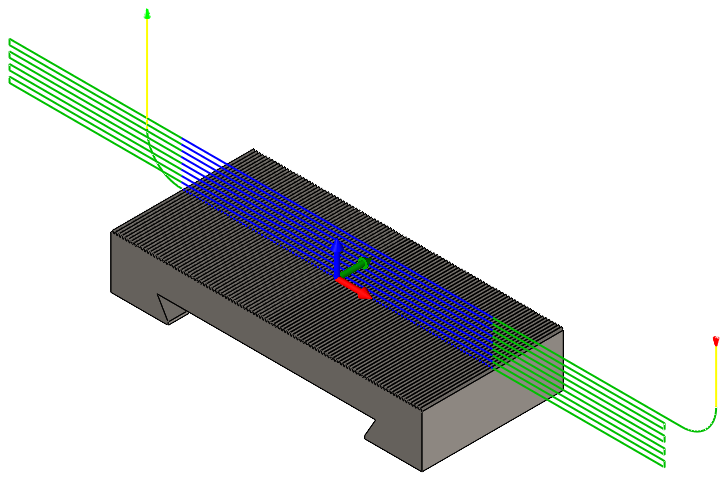
\includegraphics[width=11cm]{figures/kemenypofa_facemill_2.png}
    \caption{Az első megfogásból maradt anyag lemunkálása}
    \label{Fig:kemenypofa_facemill_2}
\end{figure}

\subsubsection{Rovátkolás}
A keménypofa funkcionáláis részének, vagyis a rovátkolásának elkészítéséhez egy gravírozó maróval történő megmunkálást választottam. A szükséges szerszámot a Hoffmann Group katalógusából választottam. A megmunkálás során vágósebesség helyett a fordulatszámot határoztam meg, mivel a szükséges vágósebességhez tartozó fordulatszámot nem tudja biztosítani a CNC megmunkálóközpont.

\begin{figure}[H]
    \centering
    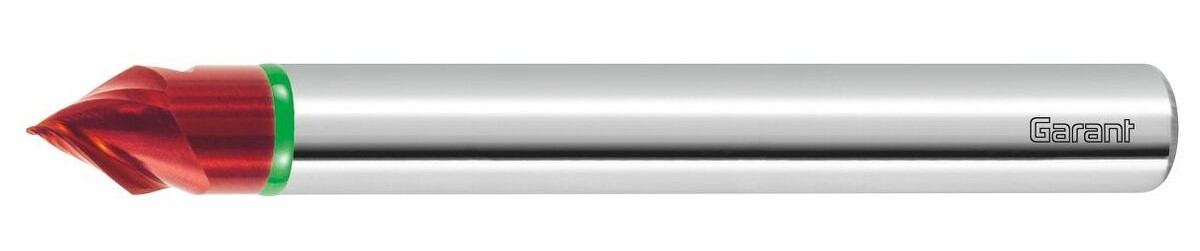
\includegraphics[width=8cm]{figures/gravir.jpg}
    \caption{A rovátkolás elkészítéséhez használt gravírozó maró}
    \label{Fig:gravir}
\end{figure}

\textbf{Adatok, paraméterek}
\begin{itemize}
    \item Megnevezés: VHM spirális gravírmaró 60° TiAlN
    \item Fordulatszám: 15000 1/min
    \item Fogankénti előtolás ($f_z$): 0,02 mm
    \item Élek száma: 2 db
\end{itemize}

Az előtolási sebességet a korábban használt \ref{Eq:facemill_vf}. egyenlettel számoltam ki.

\begin{equation*}
    v_f=f_Z\cdot z\cdot n=0,02\cdot 2\cdot 15000=600\ \dfrac{mm}{min}
\end{equation*}

\begin{figure}[H]
    \centering
    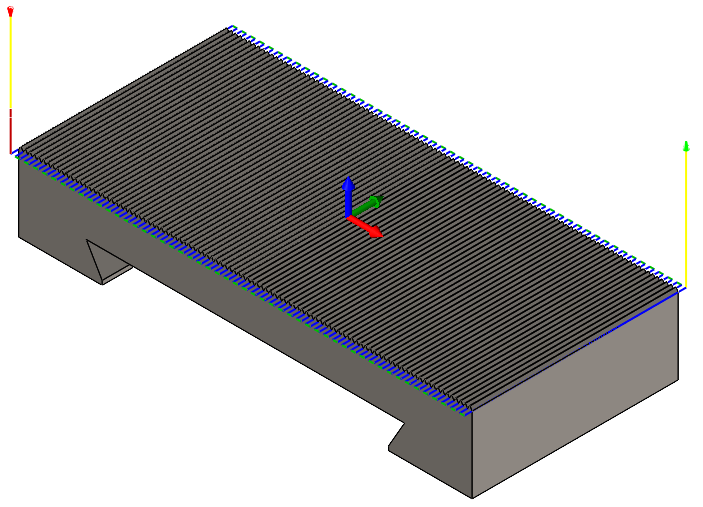
\includegraphics[width=10cm]{figures/kemenypofa_engraving.png}
    \caption{A rovátkolás szerszámpályája}
    \label{Fig:kemenypofa_engraving}
\end{figure}

\subsection{Alaptest}
Az alaptest megmunkálását 5 megfogásra tudtam felosztani. Természetesen létezik más megoldás is, azonban én ezt találtam a legoptimálisabb felosztásnak. A laborban található CNC megmunkálóközpont jelenleg 3 tengellyel rendelkezik, azonban megtalálható a laborban egy különálló, felszerelhetó 4. tengely is, mellyel lehetne csökkenteni a megfogások számát.

\subsubsection{Síkmarás - 1.}
A keménypofához használt síkmaró itt is alkalmazható lesz, ezért nem választottam új szerszámot, valamint a forgácsolási paraméterek is megfelelnek a jelenlegi megmunkáláshoz.

\begin{figure}[H]
    \centering
    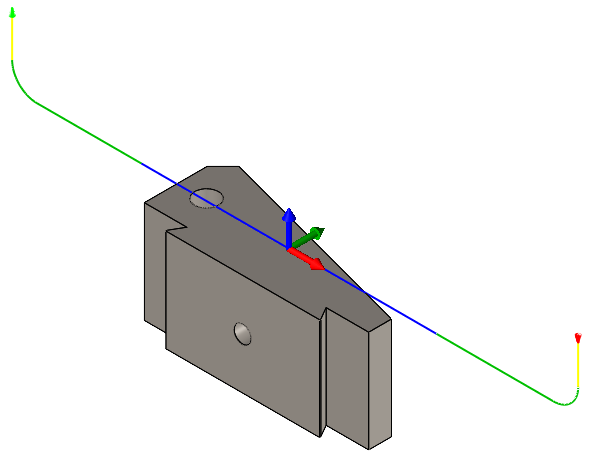
\includegraphics[width=12cm]{figures/alaptest_facemill_1.png}
    \caption{Az alaptest első síkmarásának pályája}
    \label{Fig:alaptest_facemill_1}
\end{figure}

\subsubsection{Kontúrmarás}
Az alaptest kontúrját \glqq 2D Adaptive\grqq\ megmunkálási stratégiával nagyoltam. A nagyoláshoz egy 16 mm-es átmérőjű szármarót használtam, a Kennametal katalógusából. A simítási ráhagyás értékét 0,5 mm-re határoztam meg.

\begin{figure}[H]
    \centering
    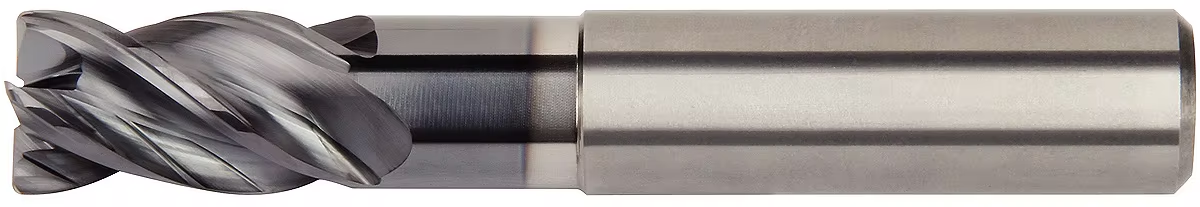
\includegraphics[width=8cm]{figures/d10_flatmill.png}
    \caption{2D Adaptive megmunkáláshoz használt maró}
    \label{Fig:d16_flatmill}
\end{figure}

\textbf{Adatok, paraméterek}
\begin{itemize}
    \item Maró: H1TE4SE1600N032HAM - KCPM15
    \item Vágósebesség: 175 m/min
    \item Fogankénti előtolás ($f_z$): 0,16 mm
    \item Élek száma: 4 db
    \item Oldalirányú fogásvétel ($a_e$): 1 mm
\end{itemize}

Az \ref{Eq:facemill_vc}. és \ref{Eq:facemill_vf}. egyenletekkel kiszámoltam a megmunkáláshoz szükséges fordulatszámot és az előtolási sebességet. 

\begin{equation*}
    n=\dfrac{v_c\cdot1000}{D\cdot\pi}=\dfrac{175\cdot1000}{16\cdot\pi}=3482\ \dfrac{1}{min}
\end{equation*}
\begin{equation*}
    v_f=f_z\cdot z\cdot n=0,16\cdot4\cdot3482=2228\ \dfrac{mm}{min}
\end{equation*}

\begin{figure}[H]
    \centering
    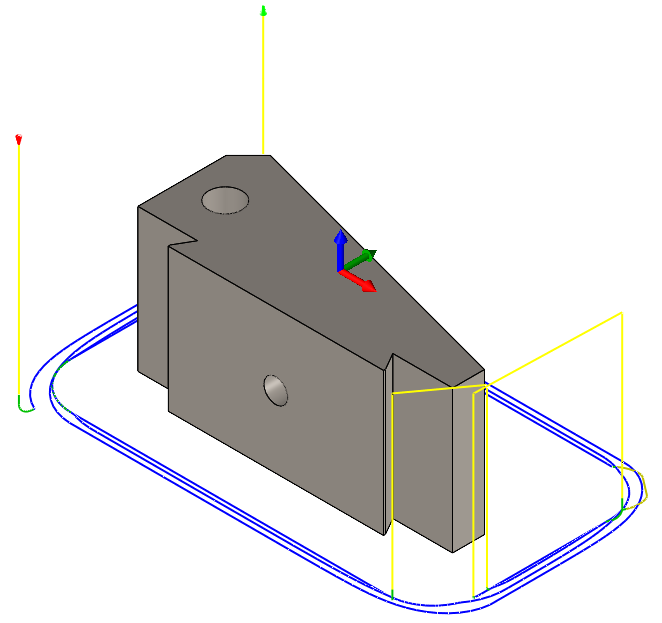
\includegraphics[width=9.5cm]{figures/alaptest_adaptive_1.png}
    \caption{2D Adaptive megmunkálás pályája}
    \label{Fig:alaptest_adaptive_1}
\end{figure}

A kontúr simítását szintén egy 16 mm átmérőjű maróval végeztem melynek a szerszámpályája az alábbi \ref{Fig:alaptest_contour_1}. ábrán látható.

\begin{figure}[H]
    \centering
    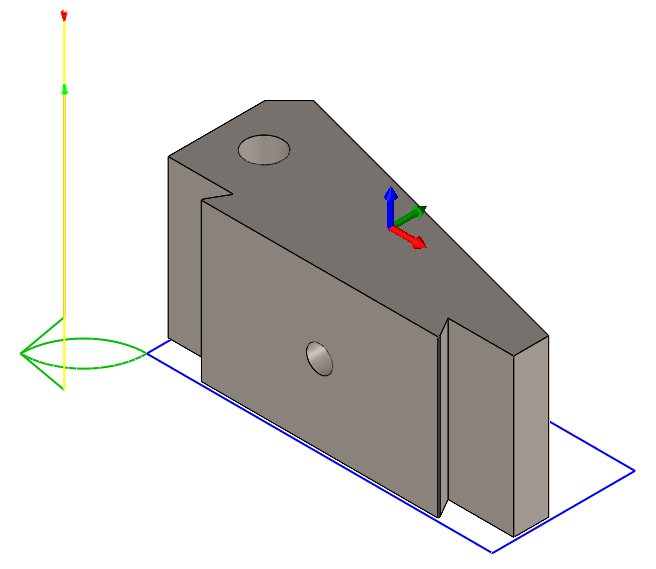
\includegraphics[width=9cm]{figures/alaptest_contour_1.png}
    \caption{Kontúr simításának szerszámpályája}
    \label{Fig:alaptest_contour_1}
\end{figure}

\subsubsection{Fúrás}
Az első megfogás utolsó művelete a visszahúzást biztosító illesztőszeg helyének fúrása. A fúrást a korábban használt 5 mm átmérőjű keményfém fúróval végeztem el. A forgácsolási paraméterek megegyeznek a korábban használttal. A fúráshoz kiemeléses mélyfúrási stratégiát alkalmaztam, mely megadott fúrási mélység után referenciapontra húzza ki a fúrót, a forgács eltávolítása érdekében. A fúró rendelkezik belső hűtéssel is, ezért az orsón keresztüli hűtést beállítottam a CAM programban.

\begin{figure}[H]
    \centering
    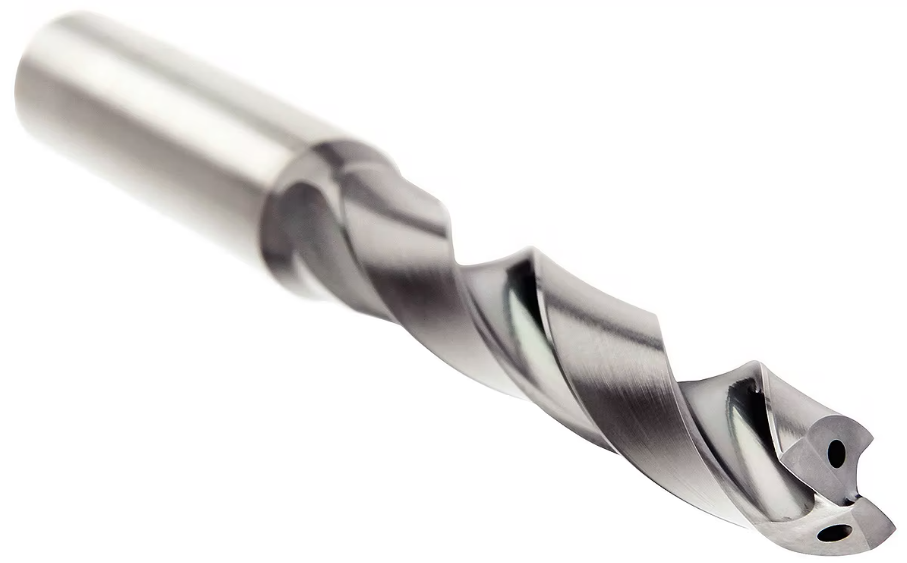
\includegraphics[width=6cm]{figures/d5_drill.png}
    \caption{Kennametal keményfémfúró}
    \label{Fig:d5_drill}
\end{figure}

\textbf{Adatok, paraméterek}
\begin{itemize}
    \item Fúró: B225A05000HPX - KCP15B
    \item Vágósebesség: 150 m/min
    \item Előtolás ($f$): 0,15 mm/ford
    \item Fúrási mélység: 5 mm
\end{itemize}

\begin{figure}[H]
    \centering
    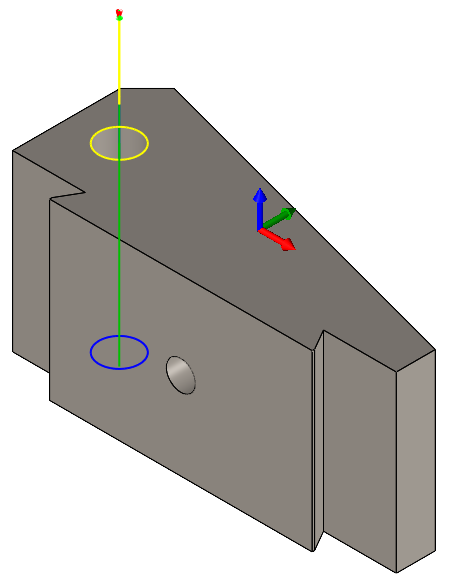
\includegraphics[width=6.5cm]{figures/alaptest_drill.png}
    \caption{Mélyfúrás szerszámpályája}
    \label{Fig:alaptest_drill}
\end{figure}

\subsubsection{Síkmarás - 2.}
A fúrást követően az alaptest első megfogása elkészült. A következő művelet a maradékanyag lemunkálása volt. Itt a korábban alkalmazott síkmarót használtam, tehát a forgácsolási paraméterek is megegyeznek a korábbiakhoz. A síkmarást 1 mm-es fogásmélységgel végeztem el.

\begin{figure}[H]
    \centering
    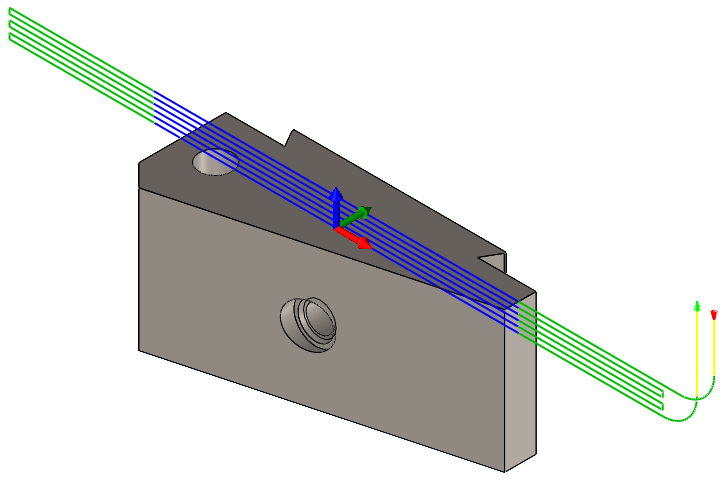
\includegraphics[width=9.5cm]{figures/alaptest_facemill_2.png}
    \caption{A visszamarás szerszámpályája}
    \label{Fig:alaptest_facemill_2}
\end{figure}

\subsubsection{Zsebmarás}
A visszamarást követően a menetes furat előkészítése történt. A menet előtti anyagrészt el kellett távolítani a könnyebb forgácsolásért, valamint a későbbiekben a könnyebb szerelhetőség érdekében. Ehhez a művelethez szintén a Kennametal katalógusából választottam egy 6 mm átmérőjű szármarót. A megmunkáláshoz helikális zsebmarási stratégiát alkalmaztam.

\begin{figure}[H]
    \centering
    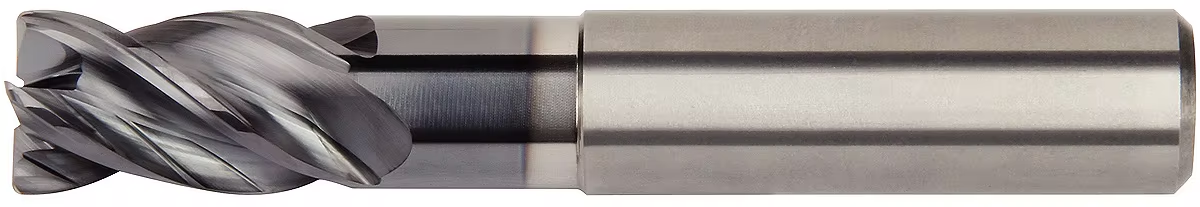
\includegraphics[width=4.5cm]{figures/d10_flatmill.png}
    \caption{Helikális zsebmaráshoz használt 6mm átmérőjű szármaró}
    \label{Fig:d6_flatmill}
\end{figure}

\textbf{Adatok, paraméterek}
\begin{itemize}
    \item Maró: H1TE4SE0600N013HAM - KCPM15
    \item Vágósebesség ($v_c$): 175 m/min
    \item Fogankénti előtolás ($f_z$): 0,02 mm
    \item Élek száma: 4 db
    \item Helikális marás süllyedése: 0,5 mm
\end{itemize}

A forgácsolási paraméterek kiszámításához a már korábban alkalmazott \ref{Eq:facemill_vc}. és \ref{Eq:facemill_vf}. egyenleteket használtam.

\begin{equation*}
    n=\dfrac{v_c\cdot1000}{D\cdot\pi}=\dfrac{175\cdot1000}{6\cdot\pi}=9284\ \dfrac{1}{min}
\end{equation*}
\begin{equation*}
    v_f=f_z\cdot z\cdot n=0,02\cdot4\cdot9284=742\ \dfrac{mm}{min}
\end{equation*}

\begin{figure}[H]
    \centering
    \includegraphics[width=8.5cm]{figures/alaptest_bore.png}
    \caption{Helikális marás szerszámpályája}
    \label{Fig:alaptest_bore}
\end{figure}

\subsubsection{Fúrás}
A helikális marás után a menet magfuratát kellett elkészíteni. Mivel a menet mérete M6, ezért az eddig alkalmazott fúrót tudtam használni. A fúrási stratégia itt is mélyfúrás volt referencia síkra történő kiemeléssel, a fúrás mélységét 5 mm-re állítottam be.

\begin{figure}[H]
    \centering
    \includegraphics[width=8cm]{figures/alaptest_drill_1.png}
    \caption{Mélyfúrás szerszámpályája}
    \label{Fig:alaptest_drill_1}
\end{figure}

A fúrást követően a menet elkészítése előtt el kellett készíteni a menet bekezdéséhez a megfelelő mértékű sarkítást. A helyes érték megállapításához az alábbi közelítő képletet alkalmaztam. Az M6 menet menetemelkedése 0,8 mm.

\begin{equation}
    h_3=0,6134 \cdot P=0,6134 \cdot 0,8 = 0,49\ mm
\end{equation}

\noindent ahol:
\begin{itemize}
    \item $h_3$: menetmélység orsón
    \item $P$: menetemelkedés
\end{itemize}

Ezzel meghatároztam a menet letörésének minimális értékét. Én a modellben 0,75 mm-es letörést alkalmaztam. Ezt a letörést egy 90°-os kúpos süllyesztővel végeztem el.

\subsubsection{Menetfúrás}
A menet elkészítéséhez a Hoffmann Group katalógusából választottam szerszámot. A választásom egy Garant bevonatos HSS menetfúróra esett. A bekezdési alakja C típusú, zsákfuratokhoz javasolt, mivel a keletkező forgácsot a menetfúró nem maga előtt tolja, hanem a csavart hornyok segítségével kivezeti a furatból.

\begin{figure}[H]
    \centering
    \includegraphics[width=9cm]{figures/m6.jpg}
    \caption{Menetfúró}
    \label{Fig:m6}
\end{figure}

\textbf{Adatok, paraméterek}
\begin{itemize}
    \item Megnevezés: GARANT Master Tap gépi menetfúró HSS-E-PM Form C M6
    \item Vágósebesség: 10 m/min
\end{itemize}

A menetfúró forgácsolási paraméterei közül elegendő csak a fordulatszámot meghatározni (\ref{Eq:facemill_vc}. egyenlet), mivel a menetemelkedés határozza meg az előtolási sebességet is.

\begin{equation*}
    n=\dfrac{v_c\cdot1000}{D\cdot\pi}=\dfrac{10\cdot1000}{6\cdot\pi}=530\ \dfrac{1}{min}
\end{equation*}

\begin{figure}[H]
    \centering
    \includegraphics[width=8cm]{figures/alaptest_tap.png}
    \caption{Menetfúrás szerszámpályája}
    \label{Fig:alaptest_tap}
\end{figure}

\subsubsection{Fecskefarok horony}
A menetfúrás elkészítése után a 4. megfogásban el tudtam készíteni a fecskefarok hornyot. A megmunkáláshoz a korábbi szerszámokat alkalmaztam, tehát a 10 mm átmérőjő szármarót, valamint a 60°-os szögmarót. Mivel mindkét szerszám volt már használva, ezért nem szükséges a forgácsolási paraméterek újraszámítása, mert azok ennél a megmunkálásnál is használhatóak lesznek.

Elsőként a fecskefarok horony nagyolását végeztem el a 10 mm-es szármaróval. Hagytam a kontúron 0,5 mm-es simítási ráhagyást. A szerszámpálya az alábbi \ref{Fig:alaptest_dovetail_1}. ábrán látható. A nagyolás elvégzése után a kontúr simítását végeztem el, melynek a szerszámpályája az \ref{Fig:alaptest_dovetail_2}. ábrán látható.

\begin{figure}[H]
    \centering
    \includegraphics[width=9cm]{figures/alaptest_dovetail_1.png}
    \caption{Fecskefarok horony nagyolás}
    \label{Fig:alaptest_dovetail_1}
\end{figure}

\begin{figure}[H]
    \centering
    \includegraphics[width=9.5cm]{figures/alaptest_dovetail_2.png}
    \caption{Fecskefarok horony oldalsimítás}
    \label{Fig:alaptest_dovetail_2}
\end{figure}

A fecskefarok horony végső alakját a 60°-os szögmaróval készítettem el. Itt 4 darab 0,5 mm-es oldalirányú fogást alkalmaztam, valamint egy 0,2 mm-es simító fogással elkészítettem a fecskefarok hornyot.

\begin{figure}[H]
    \centering
    \includegraphics[width=11cm]{figures/alaptest_dovetail_3.png}
    \caption{Fecskefarok horony elkészítése}
    \label{Fig:alaptest_dovetail_3}
\end{figure}

\subsubsection{Síkmarás - 3.}
A fecskefarok elkészítése után az utolsó megfogás köveztkezett. Ebben a megfogásban egy precíziós szögmérő segítségével 57°-os szögben rögzítettem a satuban az alkatrészt. Itt került kialakításra a szorítás biztosítására szolgáló ékszög. Ehhez a megmunkáláshoz a már korábban alkalmazott síkmarót használtam. 1 mm-es fogásmélységgel a maradék anyagot eltávolítottam a munkadarabról.

\begin{figure}[H]
    \centering
    \includegraphics[width=12cm]{figures/alaptest_facemill_3.png}
    \caption{Ékszög marásának szerszámpályája}
    \label{Fig:alaptest_facemill_3}
\end{figure}





\chapter{Összegzés}
%\todo[inline]{Legyen kb 2 oldal magyar összefoglalás, 4-5 kulcsszóval\\
%majd egy 1/2-3/4 oldalas angol összefogalás ugyanazzal a 4-5 angol kulcsszóval\\
%legyen min. 10-12 forrás}
A szakdolgozatom célja egy olyan szakítópofának a tervezése volt, ami ki tudja váltani a jelenleg a gyártótól beszerezhető típust. Szükséges volt, hogy a szakítópofa egyszerűen cserélhető legyen, rögzíteni tudja a próbatestet a szakítóvizsgálat ideje alatt, valamint, hogy tartsa a síkbeli pozícióját.

Az anyagkiválasztásnál fontos szempont volt, hogy a szakítópofa anyaga ellenálljon a vizsgálat során fellépő igénybevételnek. Figyelembe véve az alapanyagok megemelkedett kötségeit, arra a megoldásra jutottam, hogy a szakítópofát össze lehet szerelni 2 részből is, melynek egyik része, ami a szakítógéphez csatlakozik, készülhet olcsóbb, puhább anyagból is, ezért választottam a C45-ös szénacélt. Ezután kellett keresnem egy olyan szerszámacélt, melynek magas a szakítószilárdsága, ugyanakkor sűrűn alkalmazott a szerszámgyártásban, ezért a többi szerszámacélhoz képest elfogadható költséggel jár. A választásom az 1.2312 ISO számmal rendelkező 40CrMnMoS8-6 ötvözött szerszámacélra esett, amelyet leginkább hidegalakító szerszámok készítésére is használnak.

Az szükséges anyagok kiválasztása után elkezdhettem a szükséseg modellek megtervezését. Mivel korábban elhatároztam, hogy két részből fog állni a szakítópofa, keresnem kellett olyan megoldást, amely megfelelő merevséget, ugyanakkor könnyű szerelhetőséget és megfelelő pozíciótartást biztosít. A megfelelő megoldás, amely végül a végleges koncepcióba is bekerült, egy úgynevezett \glqq fecskefarok\grqq\ vezetékes megvezetés volt, melyen egy biztosító furatot készítettem, ahova egy rugó által feszített golyó tud beilleszkedni.

A modellek elkészítése után szükséges volt a modellek tesztelése, mielőtt nekiállhattam volna a gyártás tervezésének. A vizsgálatot végeselem analízissel valósítottam meg, Ansys Workbench szimulációs környezetben. A statikus vizsgálat megkezdése előtt meg kellett határoznom a szükséges kényszereket és terheléseket, melyekkel a modell szabadságfokait le tudtam kötni. A modell hálózásához szükséges paramétereket, valamint a háló sűrítését beállítottam. Ezután elindítottam a szimulációt, amely több órán keresztül végezte a komplex mátrixműveleteket. A szimuláció sikeres lefutását követően kiértékeltem az eredményeket és megállapítottam, hogy a szerkezet megfelel a követelményeknek.

A végeselem analízist követően elkezdhettem az alkatrészek gyártásának tervezését CAM szoftverben. A Gyártástechnológia laborban található 3 tengelyes megmunkálóközpontot használtam. A szükséges szerszámokat a megmunkálóközpontban szerszámtárjából, valamint a Hoffmann Group és a Kennametal katalógusaiból választottam. A szerszámpályákat sikeresen elkészítettem és gyártásra késznek minősíthetőek az alkatrészek.

\noindent Kulcsszavak: szakítóvizsgálat, végeselem analízis, számítógéppel támogatott gyártás

\section{Summary}
The goal of my thesis was to design a tensile jaw to replace the type currently available from the manufacturer. It needed to be easily replaceable, securely hold the test specimen during tensile testing, and maintain its position. Material selection was crucial for withstanding the stress during testing. I decided to construct the jaw from two parts: the part connecting to the tensile machine made from cheaper, softer C45 carbon steel, and the other from 1.2312 ISO 40CrMnMoS8-6 alloyed tool steel, known for its tensile strength and cost-effectiveness. A dovetail guide with a spring-loaded ball in a securing hole was the solution for rigidity, ease of assembly, and position maintenance. After designing, I tested the models using finite element analysis in Ansys Workbench, setting the necessary constraints and loads. Once the simulations confirmed the structure met requirements, I planned the manufacturing in CAM software, using a 3-axis machining center and tools from Hoffman Group and Kennametal catalogs. The parts were successfully created and ready for manufacturing.

\noindent Keywords: tensile strength test, finite element analysis, computer aided manufacturing


\vspace{3cm}\hspace{10cm}\textit{Horváth Milán}



\footnotesize  % Kisebb betűméret [Smaller font size]
\bibliographystyle{unsrtnat}
\bibliography{bib/mybib}
\newpage
%\printbibliography

% Függelék és mellékletek [Appendices]
\appendix
\newgeometry{inner=20mm, top=10mm, bottom=20mm, outer=25mm}
% Melléklet A
\begin{center}
    \Large\textbf{Melléklet A}
\end{center}
\begin{figure}[H]
    \centering
    \includegraphics[page=1,width=18cm]{Szakítópofa_új.pdf}
\end{figure}
%\includepdf[pages=1, scale=0.9]{Szakítópofa_új.pdf}
\newpage

% Melléklet B
\begin{center}
    \Large\textbf{Melléklet B}
\end{center}
\begin{figure}[H]
    \centering
    \includegraphics[page=1,width=18cm]{Keménypofa.pdf}
\end{figure}
%\excludeFromLocAndLot % A következő ábrákat és a táblázatokat hagyja ki a jegyzékből
                      % [Exclude following figures and tables from List Of Figures/Tables]


\end{document}
